%%%%%%%%%%%%%%%%%%%%%%%%%%%%%%%%%%%%%%%%%
% Masters/Doctoral Thesis 
% LaTeX Template
% Version 2.5 (27/8/17)
%
% This template was downloaded from:
% http://www.LaTeXTemplates.com
%
% Version 2.x major modifications by:
% Vel (vel@latextemplates.com)
%
% This template is based on a template by:
% Steve Gunn (http://users.ecs.soton.ac.uk/srg/softwaretools/document/templates/)
% Sunil Patel (http://www.sunilpatel.co.uk/thesis-template/)
%
% Template license:
% CC BY-NC-SA 3.0 (http://creativecommons.org/licenses/by-nc-sa/3.0/)
%
%%%%%%%%%%%%%%%%%%%%%%%%%%%%%%%%%%%%%%%%%

%----------------------------------------------------------------------------------------
%	PACKAGES AND OTHER DOCUMENT CONFIGURATIONS
%----------------------------------------------------------------------------------------

\documentclass[
12pt, % The default document font size, options: 10pt, 11pt, 12pt
%oneside, % Two side (alternating margins) for binding by default, uncomment to switch to one side
english,%english, % ngerman for German
singlespacing, % Single line spacing, alternatives: onehalfspacing or doublespacing
%draft, % Uncomment to enable draft mode (no pictures, no links, overfull hboxes indicated)
%nolistspacing, % If the document is onehalfspacing or doublespacing, uncomment this to set spacing in lists to single
%liststotoc, % Uncomment to add the list of figures/tables/etc to the table of contents
%toctotoc, % Uncomment to add the main table of contents to the table of contents
%parskip, % Uncomment to add space between paragraphs
%nohyperref, % Uncomment to not load the hyperref package
headsepline, % Uncomment to get a line under the header
%chapterinoneline, % Uncomment to place the chapter title next to the number on one line
%consistentlayout, % Uncomment to change the layout of the declaration, abstract and acknowledgements pages to match the default layout
]{MastersDoctoralThesis} % The class file specifying the document structure

\usepackage[utf8]{inputenc} % Required for inputting international characters
\usepackage[T1]{fontenc} % Output font encoding for international characters
\usepackage{mathpazo} % Use the Palatino font by default
\usepackage{float}
\usepackage{listings}
\lstset{
  basicstyle=\ttfamily\small,
  keywordstyle=\bfseries,
  breaklines=true,            
  frame=none,               
  numbers=none,
  commentstyle=\color{green}
}

\usepackage[backend=bibtex,style=numeric,natbib=true]{biblatex} % Use the bibtex backend with the authoryear citation style (which resembles APA)

\addbibresource{main.bib} % The filename of the bibliography

\usepackage[autostyle=true]{csquotes} % Required to generate language-dependent quotes in the bibliography
\setcounter{tocdepth}{3}
\setcounter{secnumdepth}{1}

%----------------------------------------------------------------------------------------
%	MARGIN SETTINGS
%----------------------------------------------------------------------------------------

\geometry{
	paper=a4paper, % Change to letterpaper for US letter
	inner=2.5cm, % Inner margin
	outer=3.8cm, % Outer margin
	bindingoffset=.5cm, % Binding offset
	top=1.5cm, % Top margin
	bottom=1.5cm, % Bottom margin
	%showframe, % Uncomment to show how the type block is set on the page
}

%----------------------------------------------------------------------------------------
%	THESIS INFORMATION
%----------------------------------------------------------------------------------------

\thesistitle{Analysis and development of a prompt engineering ontology} % Your thesis title, this is used in the title and abstract, print it elsewhere with \ttitle
\supervisor{Prof. Claudia d'Amato} % Your supervisor's name, this is used in the title page, print it elsewhere with \supname
\examiner{} % Your examiner's name, this is not currently used anywhere in the template, print it elsewhere with \examname
\degree{Doctor of Philosophy} % Your degree name, this is used in the title page and abstract, print it elsewhere with \degreename
\author{Simone Gramegna} % Your name, this is used in the title page and abstract, print it elsewhere with \authorname
\addresses{} % Your address, this is not currently used anywhere in the template, print it elsewhere with \addressname

\subject{Biological Sciences} % Your subject area, this is not currently used anywhere in the template, print it elsewhere with \subjectname
\keywords{} % Keywords for your thesis, this is not currently used anywhere in the template, print it elsewhere with \keywordnames
\university{{UNIVERSITÀ DEGLI STUDI DI BARI \\“ALDO MORO”}} % Your university's name and URL, this is used in the title page and abstract, print it elsewhere with \univname\\

\department{{Academic Year 2023/2024}} % Your department's name and URL, this is used in the title page and abstract, print it elsewhere with \deptname
\group{{MACHINE LEARNING}} % Your research group's name and URL, this is used in the title page, print it elsewhere with \groupname
\faculty{\href{http://faculty.university.com}{Faculty Name}} % Your faculty's name and URL, this is used in the title page and abstract, print it elsewhere with \facname

\AtBeginDocument{
\hypersetup{pdftitle=\ttitle} % Set the PDF's title to your title
\hypersetup{pdfauthor=\authorname} % Set the PDF's author to your name
\hypersetup{pdfkeywords=\keywordnames} % Set the PDF's keywords to your keywords
}

\begin{document}

\frontmatter % Use roman page numbering style (i, ii, iii, iv...) for the pre-content pages

\pagestyle{plain} % Default to the plain heading style until the thesis style is called for the body content

%----------------------------------------------------------------------------------------
%	TITLE PAGE
%----------------------------------------------------------------------------------------

\begin{titlepage}
\begin{center}
{\scshape\LARGE \univname\par}\vspace{0.5cm} % University name
\textsc{\Large     \begin{figure}[H]
    \centering
    
\includegraphics[width=.6\textwidth]{Figures/logo_UNIBA_CMYK.jpg}
    \label{logo}
    \end{figure}}%\\[0.5cm] % Thesis type

\HRule \\[0.4cm] % Horizontal line
{\huge \bfseries \ttitle\par}\vspace{0.4cm} % Thesis title
\HRule \\[1.5cm] % Horizontal line
 

 
%\vfill
\large DEPARTMENT OF COMPUTER SCIENCE\\[0.3cm]
\large Master degree in Computer Science\\[0.3cm] % University requirement text
\vfill
Thesis in\\[0.4cm]

\groupname\\[2cm] 
\begin{minipage}[t]{0.4\textwidth}
\begin{flushleft} \large
\emph{Advisor:\\[0.1cm] Prof. Claudia d'Amato} \\[0.5cm]
\emph{Co-advisor:\\[0.1cm] Dott. Roberto Barile} \\[0.1cm]
\emph{Dott. Andrea Nuzzolese} \\[0.3cm]
\end{flushleft}
\end{minipage}
\begin{minipage}[t]{0.4\textwidth}
\begin{flushright} \large
\emph{Graduating:
\\[0.1cm]
Simone Gramegna}\\
\end{flushright}
\end{minipage}\\[1cm]
\HRule \\[0.4cm]\deptname\\[2cm] % Research group name and department name
%\vfill

%{\large \today}\\[4cm] % Date
%\includegraphics{Logo} % University/department logo - uncomment to place it
 
%\vfill
\end{center}
\end{titlepage}

%----------------------------------------------------------------------------------------
%	DECLARATION PAGE
%----------------------------------------------------------------------------------------

%\begin{declaration}
%\addchaptertocentry{\authorshipname} % Add the declaration to the table of contents
%\noindent I, \authorname, declare that this thesis titled, \enquote{\ttitle} and the work presented in it are my own. I confirm that:

%\begin{itemize} 
%\item This work was done wholly or mainly while in candidature for a research degree at this University.
%\item Where any part of this thesis has previously been submitted for a degree or any other qualification at this University or any other institution, this has been clearly stated.
%\item Where I have consulted the published work of others, this is always clearly attributed.
%\item Where I have quoted from the work of others, the source is always given. With the exception of such quotations, this thesis is entirely my own work.
%\item I have acknowledged all main sources of help.
%\item Where the thesis is based on work done by myself jointly with others, I have made clear exactly what was done by others and what I have contributed myself.\\
%\end{itemize}
 
%\noindent Signed:\\
%\rule[0.5em]{25em}{0.5pt} % This prints a line for the signature
 
%\noindent Date:\\
%\rule[0.5em]{25em}{0.5pt} % This prints a line to write the date
%\end{declaration}

%\cleardoublepage


%----------------------------------------------------------------------------------------
%	ABSTRACT PAGE
%----------------------------------------------------------------------------------------

\begin{abstract}
\addchaptertocentry{\abstractname} % Add the abstract to the table of contents
This thesis explores the development of a prompt engineering ontology to improve the understanding, organization, and application of large language models (LLMs) across various domains. By providing a structured representation of prompting techniques and their relationships with LLMs, the ontology serves as a valuable resource for guiding users in effectively interacting with these advanced systems.
Large Language Models (LLMs) are AI models based on large neural networks, trained on vast amounts of text to understand and generate natural language. Those models are interesting because they are revolutionizing human-machine communication by automate complex tasks like writing, translation and coding.
However, the currently available resources reviewing LLMs and prompt engineering lack and they are fragmented because both technologies are very recent, they are evolving quickly and there is no resource that  put them together.
We propose PEO, an ontology that models the domain of LLMs and prompt engineering in order to facilitate users in choosing the most appropriate techniques for solving a problem. PEO is designed to support a wide range of users, including researchers, developers, educators, and content creators. The research adopts a systematic approach to ontology development, following the LOT (Linked Open Terms) methodology.
We adopted a systematic approach to ontology development, following the Linked Open Terms (LOT) methodology and special attention is given to ontology evaluation and publication. We evaluate the ontology according to established experimental protocols.
The outcomes suggest that it is possible to formalize knowledge about large language models and prompt engineering, inferring new useful knowledge to the users.
PEO can provide support to a wide range of users, including researchers, developers, educators, and content creators.
\end{abstract}
%----------------------------------------------------------------------------------------
%	QUOTATION PAGE
%----------------------------------------------------------------------------------------

\dedicatory{
This thesis would not have been possible without the support and encouragement of many extraordinary people. I would like to express my deepest gratitude to my supervisor, Professor Claudia d'Amato, for her invaluable guidance and to my co-supervisors: Dr. Roberto Barile and Dr. Andrea Nuzzolese for their insightful contributions and technical support. I am profoundly grateful to my family for their unwavering belief in me, to my friends for their support, and to my partner for her endless love and encouragement.\\ A special thanks goes to ChatGPT, which has been a great useful tool during these two years.

To all of you, I am eternally grateful.
}
\newpage


\vspace*{0.1\textheight}
\noindent\enquote{\itshape Per aspera ad astra}\bigbreak



%----------------------------------------------------------------------------------------
%	LIST OF CONTENTS/FIGURES/TABLES PAGES
%----------------------------------------------------------------------------------------
\hypersetup{hidelinks}

\hypersetup{linkcolor=violet}
\tableofcontents % Prints the main table of contents

\listoffigures % Prints the list of figures

\listoftables % Prints the list of tables

%----------------------------------------------------------------------------------------
%	ABBREVIATIONS
%----------------------------------------------------------------------------------------

%\begin{abbreviations}{ll} % Include a list of abbreviations (a table of two columns)

%\textbf{LAH} & \textbf{L}ist \textbf{A}bbreviations \textbf{H}ere\\
%\textbf{WSF} & \textbf{W}hat (it) \textbf{S}tands \textbf{F}or\\

%\end{abbreviations}

%-------------------------------------------------------------------------------

%----------------------------------------------------------------------------------------
%	SYMBOLS
%----------------------------------------------------------------------------------------



%----------------------------------------------------------------------------------------
%	DEDICATION
%----------------------------------------------------------------------------------------


%----------------------------------------------------------------------------------------
%	THESIS CONTENT - CHAPTERS
%----------------------------------------------------------------------------------------

\mainmatter % Begin numeric (1,2,3...) page numbering

\pagestyle{thesis} % Return the page headers back to the "thesis" style

% Include the chapters of the thesis as separate files from the Chapters folder
% Uncomment the lines as you write the chapters


%-------------------------------------------------------------------------------
\chapter*{}

\textit{Il sentiero per il Paradiso inizia all'Inferno.}

\chapter{Introduction}
\section{Context}
Artificial intelligence (AI) has increasingly become an integral part of our life, having an undeniable impact on today’s society. 
AI was defined, for the first time, in 1955 at Darthmounth Research project as problem of \textit{"making a machine behave in ways that would be called intelligent if a human were so behaving"}\cite{kaplan2019siri}. 
Over the years, the focus has not been limited to the theoretical aspect alone. The rapid development of technologies, the increase in computing power, as well as the widespread presence of sensors have enabled the application of artificial intelligence as a support technology in fields ranging from industry, healthcare, and business to education. \cite{busnatu2022clinical}
Artificial intelligence is not only applied to these sectors but can also be found in common applications such as social media, digital assistants, recommendations, online searches, and facial recognition \cite{ref1}. These are just some of the applications we interact with in our daily lives.

\subsection{Large language models in real life}
The first voice assistants began to appear starting in 2011, when Apple introduced Siri on its new iPhone model: a voice assistant capable of conversing with users in natural language. Later, other assistants were introduced to the market, including Amazon Alexa (2014) and Google Assistant (2016) \cite{ref2}. These assistants generally have the same functionalities, being able to send messages and have simple conversations with users. However, starting in November 2022, the performance of these assistants has been surpassed by a new text-based assistant released by OpenAI: ChatGPT.\\
ChatGPT, in which GPT stands for \textit{Generative Pre-trained Transformer} a family of large language models created by OpenAI that uses deep learning to generate human-like, conversational text. 
ChatGPT represents a significant leap forward compared to the AI-based assistants available on the market until that time, as it can perform more advanced tasks than its competitors, including: writing a text/letter, coding, summarizing content, and writing Excel formulas, to name a few. Subsequent versions have integrated the DALL-E 3 model, capable of generating images, and have introduced GPT-4, the latest, more powerful, and up-to-date version of the large language model. \cite{ref3}

\subsection{Prompt engineering and the role of the prompt engineer}
The advent of advanced large language models like ChatGPT and BARD not only creates new opportunities for innovation and automation but also introduces significant challenges. One of the main challenges in using these models is creating and optimize prompts (questions posed to the model by the humans) \cite{ref5} that provide the model with the right instructions to generate accurate and relevant responses. Prompt engineering specifically addresses this challenge and focuses on defining the interactions and outputs of large language models, whose core purpose is to create optimal prompts for a generative model.\cite{amatriain2024prompt}
Everything lies in shaping the prompt while considering not only the user’s goal but also the context and the specific large language model being used, these aspects are considered by a new professional role that is emerging within companies: the prompt engineer. The prompt engineer must essentially select the most appropriate prompt engineering technique for a given task, a specific large language model, and the intended goal. The aim of this thesis is to provide a new tool to support their decisions: a prompt engineering ontology developed through an experimental approach.
\section{Objectives}
This thesis sets out to bridge different domains: the prompt engineering domain, the large language models domain and the semantic web domain through the creation of an ontology within which state-of-the-art large language models and the most advanced prompt engineering techniques are represented.

\subsection{General Objectives}
\begin{itemize}
    \item \textbf{Investigating prompt engineering techniques:} The thesis includes an analysis of studies on the most recent prompt engineering techniques to represent in the ontology.

    \item \textbf{Analysis of large language model:} The thesis analyses the state-of-the-art large language models that will be represented in the ontology.

    \item \textbf{Ontology study:} Study of ontologies and their application in similar fields.

    \item \textbf{Analysis of ontology engineering techniques:} The thesis analyses various ontology engineering techniques with the aim of selecting the best approach for developing the ontology.
    
\end{itemize}


\subsection{Specific Objectives}
The specific objective of this thesis is to develop, using a state-of-the-art ontology engineering approach, a new ontology that represents prompt engineering techniques and large language models. The aim is to provide a useful tool that can be utilized not only by industry experts but also by students, content creators, and individuals without a specific background.


\section{Thesis structure}
The subsequent chapters of this thesis are structured as follows. In Chapter 2, \textbf{"Background"}, I illustrate the theoretical foundations of the work, starting with the definition of ontology. I delve into the field of ontology engineering for the development of ontologies, exploring various ontology engineering methodologies and the main design patterns available in the state of the art. Subsequently, there is an in-depth analysis of state-of-the-art large language models, which will be represented in the ontology. The chapter concludes with a section dedicated to prompt engineering and the various prompt engineering techniques applicable to large language models.\\
In Chapter 3, \textbf{"Ontology design"}, the ontology design phase is described in detail, including an in-depth explanation of the various stages of the design process. In Chapter 4, \textbf{"Ontology implementation"}, starting from the artifacts produced during the design phase, the ontology is concretely conceptualized, taking into account design patterns, and implemented. The resulting ontology is evaluated using various state-of-the-art techniques and published online. The chapter concludes with a discussion of the results achieved. Finally , in the chapter 5, \textbf{"Conclusions and future developments"}, I conclude by summarizing the work accomplished and discussing potential future developments for the ontology based on the results achieved.

\chapter{Background}

\section{Introduction on ontologies and applications}

\subsection{What is an ontology?}

In artificial intelligence an ontology is 
a formal explicit description of concepts in a domain of discourse properties of each concept describing various features and attributes of the concept, and restrictions on slots. 
The main components of ontologies are classes that represent concepts. Hierarchical relationships exist between classes, meaning a class can have one or more subclasses and super-classes. Additionally, each class is associated with attributes (slots) and restriction rules on the attribute domains (facets). Just as in object-oriented programming, classes are instantiated to create instances that make up the knowledge base.\cite{protege_ontology}
\begin{figure}[H]
    \centering
    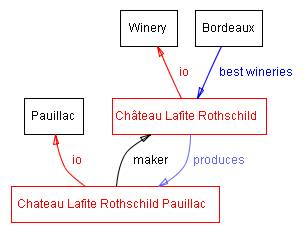
\includegraphics[width=0.5\linewidth]{Figures/fig_0.jpg}
    \caption{Example of a simple ontology in wine domain}
    \label{fig:enter-label}
\end{figure}
\subsection{Classification of ontologies}

Ontologies are useful for representing information in a hierarchical manner (through classes and subclasses), depicting the relationships between the represented information. Based on the level of generality used to describe the present domains, there are four types of ontologies:
\begin{itemize}
    \item \textbf{High-level ontologies:} High-level ontologies describe very general concepts or common-sense knowledge such as space, time, objects, and actions.

    \item \textbf{Domain ontologies:} Domain ontologies describe the vocabulary, theories, and fundamental principles that govern a specific domain.

    \item \textbf{Task ontologies:} Task ontologies describe the vocabulary related to a specific task or activity, providing a specialization of the terms introduced in the high-level ontology.

    \item \textbf{Application ontologies:} Application ontologies describe concepts related to a specific domain or task and are often derived through a specialization of domain ontologies and task ontologies.
\end{itemize}
Ontologies can differ in the way knowledge is expressed, that is, in the level of formalism used to convey terms and their meanings. Therefore, there is an additional classification:
\begin{itemize}
    \item \textbf{Highly informal ontologies:} Highly informal ontologies are expressed in natural language, and the definition of terms may be ambiguous due to the intrinsic ambiguity of natural language.

    \item \textbf{Semi-informal ontologies:} Semi-informal ontologies are expressed in a rigid and structured form of natural language, improving clarity and reducing ambiguities.

    \item \textbf{Semi-formal ontologies:} Semi-formal ontologies are expressed through formally defined artificial languages.

    \item \textbf{Strictly formal ontologies} Strictly formal ontologies are ontologies whose terms are precisely defined with formal semantics, theorems, and property proofs.
\end{itemize}

A further classification can be made based on the expressiveness the ontology aims to convey:
\begin{itemize}
    \item \textbf{Controlled vocabularies:} Controlled vocabularies are finite lists of terms representing the simplest possible notion of an ontology. A typical example is a catalog that provides only terms with an unambiguous interpretation.

    \item \textbf{Glossaries:} Glossaries are lists of terms and their meanings expressed through natural language statements. Primarily created for human use, they often consist of ambiguous statements that cannot be used by automated agents.

    \item \textbf{Thesauri:} Thesauri add semantics to glossaries by defining the relationships between terms (such as synonymy relations). Typically, they do not provide an explicit hierarchical structure, although this can be inferred from the specification of the terms.

    \item \textbf{Informal Is-A hierarchies:} Informal Is-A hierarchies are ontologies in which generalization and specialization are achieved even though there is no strict "sub-class" hierarchy. They include various ontologies available on the Web.

    \item \textbf{Formal Is-A hierarchies:} Formal Is-A hierarchies are ontologies in which concepts are organized according to a strict subclass hierarchy, and the concept of inheritance can always be applied.

    \item \textbf{Frames:} Frames are ontologies in which concepts are described in terms of their characteristic properties. The inclusion of properties in the description of concepts becomes more interesting when inheritance can be applied, allowing properties to be specified for a more general concept and then inherited.

    \item \textbf{Value restrictions:} Value restrictions allow for applying constraints on the values associated with properties.

    \item \textbf{General logical restrictions:} General logical restrictions are usually written in a highly expressive ontological language that allows for the specification of first-order logic constraints on concepts and properties.
    
\end{itemize}
The classifications presented, taken from the Italian study "Ontologie e Linguaggi Ontologici per il Web Semantico" \cite{canfora2004ontologie}, are useful for introducing and better understanding the domains and ways in which ontologies are applied.

\subsection{Applications of ontologies}
Ontologies, therefore, offer the possibility to represent information at various levels in a formal and expressive manner, and for these reasons, they are primarily applied in the following domains: \cite{leonels2023ontology}
\begin{itemize}
    \item \textbf{Information retrieval:} Ontologies can be used to improve the accuracy of search results by helping to understand the meaning of terms and relationships between them.

    \item \textbf{Knowledge management:} Ontologies can help organize and manage knowledge in a more structured and systematic way. They can also facilitate the sharing and reuse of knowledge across different systems and applications.

    \item \textbf{Semantic web:} Ontologies are a key component of the Semantic Web, which aims to make web content machine-readable and understandable by computers.

    \item \textbf{Natural language processing:} Ontologies can be used to improve natural language processing by providing a framework for understanding the meaning of words and sentences.

    \item \textbf{Robotics:} Ontologies can be used to enable robots to better understand their environment and perform tasks more efficiently and accurately.

    \item \textbf{Healthcare:} Ontologies can be used to improve healthcare by providing a standardized way to represent medical knowledge and improve the interoperability of healthcare systems.

    \item \textbf{E-commerce:} Ontologies can be used to improve product search and recommendation systems by providing a more structured and accurate representation of products and their attributes.
\end{itemize}
There are numerous studies and projects in which ontologies and methods for applying ontologies in the mentioned fields have been developed. Regarding information retrieval, the study "The use of ontologies for effective knowledge modelling and information retrieval" \cite{munir2018use} analyzes ontology-based approaches for information retrieval and query formulation on databases. In "Ontology-to-database mapping," a mapping is performed between a relational database and an existing ontology. The mapping is done by representing constructs present in the relational database schema as constructs in the ontology schema and can be achieved using various methods and approaches, including the R2O (Relational to Ontology) language \cite{khan2011r2o}. Another approach described is "Database-to-ontology transformation," where it is assumed that only the relational database exists, and the ontology is created by applying transformation rules. \\
In natural language processing, ontologies can be used to make inferences and to derive rules for semantic interpretation and question-answering systems. In "Natural Language Processing methods and systems for biomedical ontology learning" \cite{liu2011natural} ontologies are applied for the semantic interpretation of clinical documents that is useful to improve questions comprehension and retrieval of correct information.
The use of ontologies in healthcare can be useful for providing information to doctors and patients, improving the quality of medical services. To this end, the study *"Ontology-based Public Healthcare System in Internet of Things"* \cite{kumar2015ontology} describes the implementation of a healthcare information management system based on the Internet of Things. The ontology represents all the concepts and relationships between them necessary to semantically represent the information. The information pertains to healthcare personnel, disease diagnosis, and patient clinical data.\\
As seen in the previously mentioned case, ontologies can be used to represent real-time information, one example of application is robotics. In the paper "OntoSLAM: An Ontology for Representing Location and Simultaneous Mapping Information for Autonomous Robots" \cite{cornejo2021ontoslam} the ontology "OntoSLAM" is created to track in real time all the informations related to robots, those informations are gathered from the robot control system, sensors and actuators. Robots in the environment exchange those informations using a web repository.\\
The presented examples are just a few, but there are thousands of projects where ontologies have been created in a wide range of fields. For this reason, there are online repositories of ontologies, including: \href{https://www.w3.org/wiki/Lists_of_ontologies}{W3.org}, \href{https://archivo.dbpedia.org/list}{DBpedia}, \href{https://agroportal.lirmm.fr/ontologies?search=o}{AgroPortal} and \href{https://bioportal.bioontology.org/ontologies}{BioPortal}. 

\section{Ontology engineering}

\subsection{Competency questions and ontology conceptualization}
The definition of requirements and the subsequent conceptualization are two fundamental steps in ontology design, as they are essential for establishing the objectives, scope of the ontology, and the classes within it. To define the scope and the problems that the ontology should be able to address, designers use competency questions (CQs), which are a set of questions written in natural language that the ontology should be able to answer using its axioms. \cite{malheiros2013method}
In the development of an ontology for noise pollution monitoring \cite{espinoza2020using}, the following competency questions have been defined:

\begin{table}[H]
    \centering
    \begin{tabular}{|>{\raggedright\arraybackslash}p{1cm}|>{\raggedright\arraybackslash}p{6cm}|>{\raggedright\arraybackslash}p{6cm}|}
        \hline
        \textbf{Id} & \textbf{Competency question} & \textbf{Answer} \\ \hline
        \textbf{CQ1} & Which is the measured noise level in a specific moment and location? & The detected noise level during April in location with coordinates 40.42, – 3.69, 648 is 67.4 dB. \\ \hline
        \textbf{CQ2} & Which is the location of a specific measurement station? & The location of the measurement station “Paseo de Recoletos” is 40.42, – 3.69, 648 (Longitude, Latitude, Altitude) \\ \hline
        \textbf{CQ3} & In which day interval the noise level has been detected? & The noise level Ld has been detected in the time interval between 07:00 to 19:00. \\ \hline
        \textbf{CQ4} & Which was the last calibration sensor date? & The datetime, for example, 2017-04-21T14:00:00+01:00 \\ \hline
    \end{tabular}
    \caption{Competency Questions noise pollution ontology}
\end{table}

Each competency question must correspond to a natural language answer that "simulates" the response provided by the ontology. Of course, competency questions are not mandatory for developers but can be used for the creation of methods to translate CQs into ontology queries. An example of a manual translation of a competency question has been done on the African Wildlife Ontology \cite{keet2020african}, where the competency question \textit{"Which plants eat animals?"} was translated into SPARQL-OWL language, resulting in the following code \cite{wisniewski2019analysis}.

\begin{verbatim}
SELECT DISTINCT ?eats
WHERE {
  ?eats rdfs:subClassOf awo:plant, [
    a owl:Restriction ;
    owl:onProperty awo:eats;
    owl:someValuesFrom awo:animal
  ].
  FILTER(?eats != owl:Nothing)
}
\end{verbatim}

The next step, once the competency questions have been defined, is the conceptualization of the ontology, which is useful for defining the classes and the hierarchy among them. There are three approaches to conceptualization:
\begin{enumerate}
    \item \textbf{Top-down:} top-down development process starts with the definition of the most general concepts in the domain and subsequent specialization of the concepts.
    \item \textbf{Bottom-up:}  bottom-up development process starts with the definition of the most specific classes, the leaves of the hierarchy, with subsequent grouping of these classes into more general concepts.
    \item \textbf{Combination:} development process is a combination of the top-down and bottom-up approaches: We define the more salient concepts first and then generalize and specialize them appropriately.
\end{enumerate}
The conceptualization can be carried out by stating classes in a formal system or can be done using diagrams, in this case is important to defined the notation that will be used. 
% vedere se devo aggiungere altro

\subsection{Ontology languages}
Once the requirements have been defined and the classes and entities that make up the ontology have been established, the implementation phase begins. There is a set of languages available for implementing ontologies, with the main standards being RDF (Resource Description Framework) and OWL (Web Ontology Language).\\
RDF is a standard model for data interchange on the Web, it  has features that facilitate data merging even if the underlying schemas differ, and it specifically supports the evolution of schemas over time without requiring all the data consumers to be changed. RDF extends the linking structure of the Web to use URIs to name the relationship between things as well as the two ends of the link (this is usually referred to as a “triple”). Using this simple model, it allows structured and semi-structured data to be mixed, exposed, and shared across different applications.\cite{rdf}\\ 
OWL is a family of knowledge representation for ontologies, the latest version OWL2, born in 2009, is used to build ontologies representing classes, properties, individuals, and data values that are stored as Semantic Web documents.\cite{owl2} 
\subsection{Ontology engineering methodologies}
The definition of requirements through competency questions and the subsequent conceptualization and implementation fall within the ontology design process, which is studied in ontology engineering. By definition the ontology engineering  is the discipline that investigates the principles, methods and tools for creating and maintaining ontologies. An ontology engineering methodology caters the methodological aspect of ontology development and it gives a set of guidelines and activities to develop ontologies.\cite{iqbal2013analysis}
Over the years, various ontology engineering methods have been proposed; below, I analyze the main methods available in the state of the art.

\subsubsection{METHONTOLOGY}
The first methodology analyzed is \textit{METHONTOLOGY} \cite{fernandez1997ontological} that proposes a structured method which consists of six steps: 
The process begins with the Specification phase, where the goal is to produce an ontology specification document. This document can be informal, semi-formal, or formal, and is written either in natural language or using competency questions to outline the main requirements and scope of the ontology. Next is the Knowledge Acquisition phase, which involves gathering all relevant knowledge related to the domain. This is achieved through various techniques, such as text analysis, brainstorming, interviews, and reviewing existing similar ontologies. The aim is to collect a comprehensive set of information that will serve as the foundation for the ontology. The Conceptualization phase follows, where the acquired knowledge is organized into a conceptual model. This model effectively structures the domain knowledge, describing both the problem and its proposed solution in a coherent manner. During the Integration phase, the methodology encourages reusing and integrating existing ontologies rather than developing new ones from scratch. This step is crucial for ensuring consistency and coherence, as it involves checking libraries of ontologies to find definitions of terms that match the semantics identified in the conceptualization phase. The Implementation phase is where the actual construction of the ontology takes place. Here, the developer selects the appropriate environment and tools to implement the ontology based on the specifications and conceptual model developed in the earlier phases. Finally, the Evaluation phase ensures the quality and correctness of the ontology. This step involves both verification, to confirm that the ontology is technically sound, and validation, to guarantee that the ontology meets the specified requirements. The methodology has the following advantages: 
\begin{itemize}
    \item Methontology identifies all the activities required to develop an ontology, including planning, specification, conceptualisation, formalisation, integration, implementation, evaluation and documentation. 

    \item It proposes the use of an evolutionary prototype life cycle, which allows definitions to be modified, added or removed at any time.

    \item It encourages the reuse of already existing ontologies, which can speed up development and ensure consistency with other projects. 
\end{itemize}
and the following disadvantages:
\begin{itemize}
    \item Methontology is very detailed and rigorous, which can be time and resource consuming, especially for smaller projects, it may be excessive compared to the needs of the project.

    \item The methodology can be complex to master for those without experience in ontology development, as it requires familiarity with several specific techniques and tools.

    \item The methodology has been developed in 1997, making it outdated by today standards. Since its creation, there have been significant advancements in both ontology engineering and related technologies, such as the Semantic Web, Linked Data, and agile methodologies.

    \item The methodology was created before the widespread adoption of agile development practices, which are now a common approach in software and ontology engineering. This makes it less flexible for fast-paced, iterative development environments.
\end{itemize}

\subsubsection{NeOn methodology}
Another proposed methodology is the \textit{NeOn methodology}\cite{neon1}\cite{neon2} which provides guidance for all key aspects of the ontology engineering process. The concepts underlying this methodology are: scenarios, collaborative ontology development, reuse of ontological and non-ontological resources and evolution of networked ontologies. The ontology design is based on nine scenarios:
\begin{enumerate}
    \item \textbf{Scenario 1: From specification to implementation} The ontology network is developed from scratch, developers should specify ontology requirements and search for potential resources to be reused. 

    \item \textbf{Scenario 2: Reusing and re- non-ontological resources}  Developers should carry out the NOR reuse process for deciding, according to the ontology requirements, which NORs can be  reused to build the ontology network. 

    \item \textbf{Scenario 3: Reusing ontological resources} Developers use ontological resources, ontology modules and ontology statements to build ontology networks. 

    \item \textbf{Scenario 4: Reusing and re-engineering ontological resources} Ontology developers reuse and re-engineer ontological resources

    \item \textbf{Scenario 5: Reusing and merging ontological resources} This scenario arises when several ontological resources in the same domain are selected for reuse, and developers wish to create a new ontological resource with the selected resources

    \item \textbf{Scenario 6: Reusing, merging and re- engineering ontological resources} Ontology developers reuse, merge, and re-engineer ontological resources. This scenario is similar to Scenario 5, but here developers decide to re- engineer the set of merged resources

    \item  \textbf{Scenario 7: Reusing ontology design patterns (ODPs)} Ontology developers access repositories to reuse ODPs

    \item \textbf{Scanrio8: Ontology developers access repositories to reuse ODPs} Ontology developers restructure (e.g., modularize, prune, extend, and/or specialize) ontological resources to be  integrated in the ontology network. 

    \item \textbf{Scenario 9: Localizing ontological resources} Ontology developers adapt an ontology to other languages and culture communities, thus obtaining a multilingual ontology.

\end{enumerate}
The scenarios presented are not a rigid workflow, they are more like a variety of pathways for developing ontologies and they  cover commonly occurring situations, for example, when available ontologies need to be re-engineered, aligned, modularized, localized to support different languages and cultures, and integrated with ontology design patterns and non-ontological resources, such as folksonomies or thesauri.\cite{suarez2011neon}\\

The \href{http://neon-project.org/nw/Welcome_to_the_NeOn_Project.html}{Neon project} offers to developers a tool called \href{http://neon-toolkit.org/wiki/Main_Page.html}{NeOn toolkit}: an open-source multi-platform ontology editor which supports the Web Ontology Language OWL2 and features basic editing and visualization functionality.\cite{erdmann2011overview}\\
\begin{figure}[H]
    \centering
    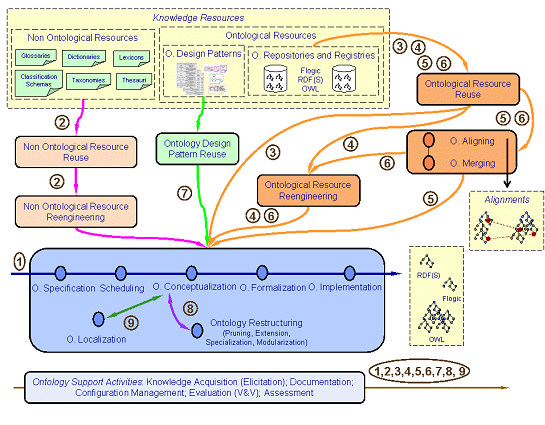
\includegraphics[width=0.5\linewidth]{Figures/fig_2.png}
    \caption{NeOn methodology scenarios}
    \label{fig:enter-label}
\end{figure}
The NeOn methodology has the following advantages:
\begin{itemize}
    \item It identifies nine different scenarios for building ontology networks, which can be combined depending on the project’s needs, this contrasts with more rigid methodologies like METHONTOLOGY.

    \item It supports the reuse and re-engineering of both ontological and non-ontological resources, which can save time and effort by leveraging existing knowledge bases, reducing the need to build everything from scratch.

    \item By basing its structure on real use cases and generalizing from them, the NeOn methodology covers practical needs encountered in ontology development projects.
\end{itemize}
But NeOn has the following disadvantages:
\begin{itemize}
    \item The flexibility and comprehensive nature of the methodology can make it more complex to apply, especially for teams without significant prior experience in ontology development. 

    \item Although NeOn is designed for building large-scale networks, the actual process of merging and aligning different ontologies can be challenging, especially when ontologies come from diverse sources with differing structures and standards.

    \item The methodology is meant to be technology-independent, in practice, it may require specific tools to implement the processes effectively, and these tools might not always be accessible or easy to use for all teams.
\end{itemize}

\subsubsection{Extreme design}
While the NeOn methodology is scenario-based, the eXtreme Design methodology \cite{presutti2009extreme} is based on a sequence of tasks inspired by the principles of agile development in software engineering. eXtreme Design involves the client in order to gather complete requirements without making incorrect assumptions. This interaction is useful for defining competency questions and customer stories that detail the use of the ontology, supported by contextual statements that make implicit knowledge explicit. The principles of eXtreme Design not only focus on the client but also provide clear guidelines to designers regarding the design and organization of work. In particular, the design must be modular and task-oriented, focusing on the specifications defined in the competency questions. These competency questions are used in the development of unit tests during the testing phase, verifying the compliance of the ontology with the user stories. Tests are generally conducted using SPARQL queries that encode the competency questions. Throughout the development phase, the designers are organized according to the \textit{pair design}, where the design team is divided into pairs that must collaborate, sharing knowledge and integrating the various parts of the ontology developed. Based on the principles illustrated, eXtreme design defines adisci task: 
\begin{enumerate}
    \item \textbf{Task 1. Get into the project context:} The development process begins by aligning the designers and domain experts, who may have different backgrounds and terminologies. The goal is twofold: to familiarize the customer with the project's methods and tools, and to provide the designers with an understanding of the problem, scope, and initial terminology, establishing a collaborative environment for sharing documentation and discussing modeling issues.

    \item \textbf{Task 2. Collect requirement stories:} The customer writes stories starting from real scenarios in order to sample the typical facts that should be stored in the ontology.

    \item \textbf{Task 3. Select a story that has not been treated yet:} Each pair of designers selects a story to focus on for the next iteration, creating a new wiki page with the story's title and content based on the information from the card.

    \item \textbf{Task 4. Transform the story into CQs:} Starting from the wiki created in the previous task, designers create a sequence of competency questions, this task involves customer for having feedback/clarifications.

    \item \textbf{Task 5. Select a CQ that has not been treated yet:} The iteration continues by selecting one of the CQs.

    \item \textbf{Task 6. Match the CQ to GUCs:} This task aims to identify candidate Content Patterns (CPs) based on the Competency Questions (CQs) that express part of the Logical Unit of Concern (LUC). Matching can be done with tool support, such as keyword-based searching, or manually by designers familiar with available CPs.

    \item \textbf{Task 7. Select the CPs to reuse:} The goal of this task is to select which of those patterns should be used for solving the modeling problem. 

    \item \textbf{Task 8. Reuse and integrate selected CPs:} . The term “reuse” here refers to the application of typical operation that can be applied to CPs i.e. import, specialization, and composition. 

    \item \textbf{Task 9. Test and fix:} The goal of this task is to validate the module by ensuring it aligns with the Competency Questions (CQs) just modeled. This process involves several steps: first, the CQ is transformed into a unit test, such as a SPARQL query, then, the module is populated with sample data based on the story, and the test is run. If the result isn't as expected, the module is revised and the test is rerun until it passes and once all tests linked to the story have been successfully completed, the designers can move on to the next task. If any CQ remains unaddressed, they return to an earlier task to make adjustments.

    \item \textbf{Task 10. Release module:} This tasks ends the development phase and releases an ontology module having an URI shared with the whole team and on web repositories.

    \item \textbf{Task 11. Integrate, test and fix:} After the module is released it has to be integrated with the other modules that constitute the ontology. 
\end{enumerate}
Once the eleven tasks have been completed, the release of the new version of the ontology takes place. 
The eXtreme design methodology has the following advantages:
\begin{itemize}
    \item The methodology supports collaboration and modular ontology development, allowing teams to work on different parts of the ontology in parallel, which is especially useful for large and distributed projects.

    \item It employs a test-driven approach, where competency questions and contextual statements serve as the basis for unit testing the ontology, ensuring that each component meets its intended purpose before moving forward.

    \item The methodology emphasizes constant interaction with domain experts and stakeholders to ensure that the ontology meets the intended use and requirements. This minimizes assumptions and ensures that implicit knowledge is captured
\end{itemize}
But there are some disadvantages:
\begin{itemize}
    \item The methodology's iterative, test-driven nature may be overkill for smaller ontology projects, where a simpler, more direct approach could be more efficient.

    \item Effective use of XD relies on the availability of supporting tools, such as the NeOn Toolkit and its XD plugin. While these tools are valuable, they may limit accessibility if they are not well-maintained or widely available.
\end{itemize}

\subsubsection{LOT Methodology}
The \textit{LOT Methodology} (Linked Open Terms) \cite{poveda2022lot} introduces a lightweight industrial-oriented method for developing ontologies. The methodology is compatible with software development techniques, in fact it is inspired by the agile methodology and it defines a basic workflow consisting in four steps:
\begin{figure}[H]
    \centering
    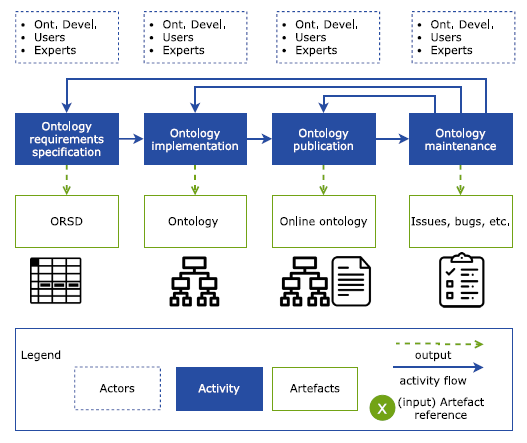
\includegraphics[width=0.7\linewidth]{Figures/fig_3.png}
    \caption{LOT methodology base workflow}
    \label{fig:enter-label}
\end{figure}


\subsubsection{Ontology requirements specification}
In this phase there is the definition of of the domain that the ontology should model, the goal of the ontology and the implementation language. In detail there are seven steps as shown below:
Initially, use case specifications are created in collaboration with domain experts, users, and ontology engineers. These use cases describe scenarios in which the ontology will be utilized, expressed in natural language. Next, data exchange identification is carried out, where the necessary documentation and resources related to the domain are gathered and compiled into a set of documents. This provides a foundation for understanding the context and requirements of the ontology. The purpose and scope of the ontology are then identified with input from users and domain experts. The purpose clarifies the reason for creating the ontology, while the scope defines the aspects of the domain that will be represented. Subsequently, a set of functional ontological requirements is proposed, often in the form of competency questions (CQs) or natural language statements. These requirements outline what the ontology should be able to answer or represent. Ontology experts then review these functional requirements to ensure their correctness and completeness, addressing any ambiguities and verifying consistency with the defined purpose and scope. Following this, the Ontology Requirements Specification Document (ORSD) is formalized. This document consolidates all the information, competency questions, and functional requirements defined in the earlier phases, serving as a comprehensive reference for the ontology development. In some cases, an optional activity is conducted where the functional ontology requirements are further formalized into test cases, expressed in SPARQL queries. This step helps in validating that the ontology meets the specified requirements through structured testing.

\subsubsection{Ontology implementation}
In this phase the ontology is implemented using a formal language, first there is the conceptualization in which there is the definition of classes, sub-classes, relationships and axioms. In the encoding phase there is the actual creation of the ontology using an implementation language, in this phase is useful to take into account other similar ontologies that could be reused. Once the whole ontology is completed it can be evaluated according different evaluation criteria. 

\subsubsection{Ontology publication}
In this phase the ontology is published online, making it accessible and searchable by users. Before publishing the ontology online, it is necessary to identify the version to be released, document the ontology using human-readable HTML pages, and finally publish the ontology online according to W3C guidelines.\cite{ontology_online}

\subsubsection{Ontology maintenance}
The last step is the ontology maintenance, in this phase once the ontology is published online there is bug detection but it also useful in order to update the ontology according new requirements.

\subsubsection{Application of LOT methodology}
Despite being introduced recently, the LOT methodology has been successful and has been applied in several projects, both in research and in the industrial field, for the development of ontologies. In the industrial and manufacturing sector, the ontology \textit{SAREF4INMA} \cite{de2020saref4inma} has been developed to describe equipment, materials, products, factories and manufacturing processes in a structured way. The industry is not the only sector where an ontology developed with the LOT method can be applied. In Spain, specifically in Madrid, an ontology has been developed to represent the Bus Public Transport system. \cite{ruckhaus2023applying} The ontology represents information on lines, routes, journey patterns and their timetables, stops on each route, information on expected bus arrival times for each stop, and information on planned and unplanned incidents that may affect the bus routes and their journeys. Still in Spain the LOT methodology has been successfully used in the development of a noise pollution ontology.\cite{espinoza2020using} The ontology integrates data from IoT sensors in the city and establishes semantic relationships between them. The LOT methodology has been used also in artificial intelligence research field, the \textit{HALO ontology} \cite{nananukul2024halo} has been creating for representing hallucinations in large language models. In the ontology there are classes for representing LLMs, hallucinations (with subclasses), prompts and responses. The ontology consists of two modules and was created from a dataset of 40 known prompts designed to generate hallucinations. Each prompt was given as input to three large language models: ChatGPT, BARD, and Claude.
\begin{figure}[H]
    \centering
    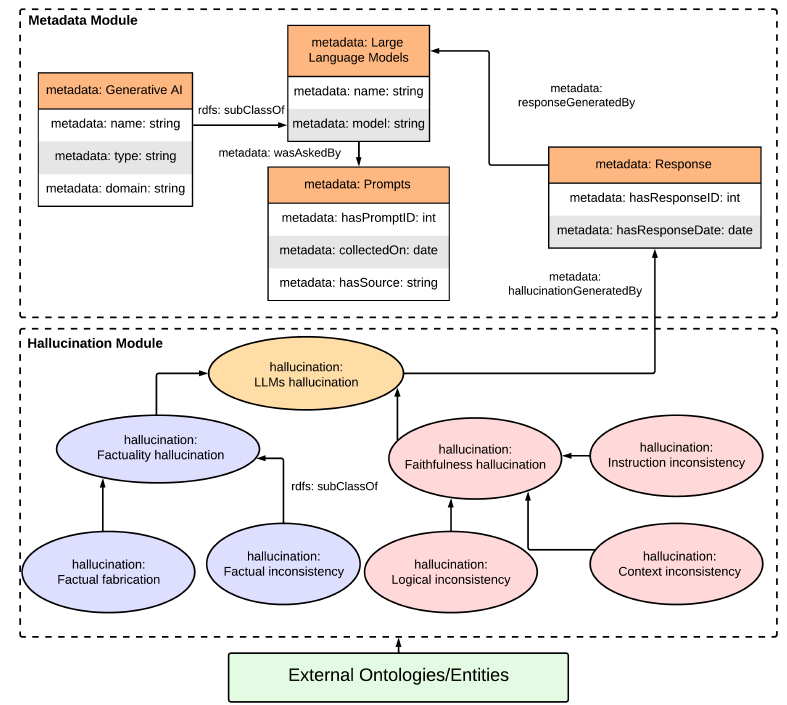
\includegraphics[width=0.7\linewidth, height=8cm]{Figures/fig_4.png}
    \caption{HALO ontology}
    \label{fig:enter-label}
\end{figure}
The LOT methodology has the following advantages:
\begin{itemize}
    \item The LOT methodology is designed to be lightweight and agile, which allows for faster iterations and easier integration with software development practices and it is particularly well-suited for projects that need rapid, iterative development.

    \item The methodology provides a structured approach, including well-defined steps such as ontology requirements specification, implementation, publication, and maintenance.

    \item It offers flexibility by combining various techniques ( competency questions, natural language statements ...) to define requirements and allows for different levels of formality depending on the project.

    \item Many open source ontologies have been developed successfully using LOT methodology for example the HALO ontology, the public transport ontology and may others described previously.
\end{itemize}
but the LOT methodology has two disadvantages:
\begin{itemize}
    \item LOT encourages the reuse of existing ontologies, but this can be challenging due to the potential inconsistencies and heterogeneity of reused ontologies. The methodology does not fully address how to resolve these issues.

    \item The emphasis of LOT on formal validation processes (such as the use of SPARQL queries) may not be sufficient for certain complex domains or non-technical stakeholders.
\end{itemize}

\subsection{Ontology engineering using large language models}
The methodologies analyzed for ontology design involve users, domain experts, and ontology engineers, but do not include the use of advanced tools based on artificial intelligence, such as large language models. The spread of large language models has opened a new path for the design and construction of knowledge graphs and ontologies in an automatic or semi-automatic manner. The study "From human experts to machines: An LLM supported approach to ontology and knowledge graph construction"\cite{kommineni2024human} introduces a semi-automatic pipeline for the construction of knowledge graphs. There are six phases in the proposed pipeline.
The process begins with the data collection phase, which does not involve the use of large language models (LLMs). Instead, domain experts generate a dataset and a set of publications relevant to the topic under study.
In the next phase, known as competency question (CQ) generation, ChatGPT-3.5 is utilized to create competency questions. These questions are designed to describe the data collected in the previous phase at an abstract level. Domain experts provide inputs to the LLM to generate these questions, which are then evaluated by two domain experts to ensure their relevance and accuracy. Following this, the ontology creation phase is initiated. It builds on the competency questions generated earlier. This phase involves two steps: in the first step, a prompt is created that includes a competency question, the expected output, and a set of instructions. In the second step, the LLM is provided with a basic ontology structure containing the concepts and relationships derived from the competency questions.
The CQ answering phase involves applying text processing techniques to extract answers to the competency questions. These answers are used to enrich the ontology and provide a deeper understanding of the dataset.
During the knowledge graph (KG) construction phase, the competency questions, their answers, and the ontology generated by the LLM are combined and provided as input to the LLM. The prompt for this phase focuses on extracting entities, relationships, and concepts and mapping them onto the ontology, thereby creating a comprehensive knowledge graph.
Finally, in the evaluation phase, the LLM evaluates the competency questions and the constructed knowledge graph by comparing them to a ground truth generated by human evaluators. The LLM assigns a score based on the alignment of the generated knowledge graph with the human-generated ground truth.
The presented method enabled the creation of a fairly complex ontology consisting of 45 classes, 41 relations, and 365 axioms. However, it required significant computational resources, as an 80GB NVIDIA A100 GPU machine was used. \\
Another approach for ontology learning using large language models is NeOn-GPT.\cite{fathallah2024neon} Starting from the NeOn methodology, the methodology is converted to a series of prompts to ChatGPT-3.5, these prompt are created using prompt engineering techniques and they are used first to generate ontology specification and competency questions. ChatGPT-3.5 is used also to generate a conceptual model of the ontology in the form of subject-relation-object triples and to generate implementation code. Once the code is generated, there is the syntax validation using the RDFLib python library\cite{rdflib} and the consistency check in order to check logical inconsistencies. The final step is the pitfall resolution for checking circular axioms and missing disjointedness using OOPS API. The presented methodology is an evolution of the NeOn methodology, in which all tasks traditionally performed by the developer are delegated to ChatGPT. This includes identifying requirements, writing competency questions, conceptualizing, and implementing the ontology.\\
ChatGPT can be used not only for the creation of ontologies but also for the creation of more complex knowledge graphs, specifically Hyper-Relational Knowledge Graphs, as discussed in the study "Construction of hyper-relational knowledge graph using pre-trained large language models".\cite{datta2024construction} Hyper-relational knowledge graphs unlike the normal knowledge graphs incorporate additional qualifiers or attribute-value pairs\cite{hyper}, in the study starting from HyperRED dataset, a dataset about different topics , the hyper relational knowledge graph is built including in prompts the data from the dataset. Prompts are generated using Chain-of-Thoughts prompt engineering technique (CoT) and in order to evaluate the result generated, BERTScore is choose as a metric. The results obtained were not satisfactory, as the other algorithm(CubeRE)for extracting hyper-relational information was not surpassed.\\
In general, large language models have shown promising potential  in automating and enhancing the processes of ontology and knowledge graph construction replacing the ontology engineer in different tasks.

\newpage
\subsection{Ontology design patterns}
In ontology engineering, ontology design patterns (ODPs) are a powerful approach, design to address recurring problems in the development of ontologies.\cite{hitzler2016ontology}
According to the official definition given in the paper \textit{"Ontology Design Patterns"}, an ontology design pattern is: a modelling solution to solve a recurrent ontology design problem.\cite{gangemi2009ontology} These patterns encapsulate best practices, enabling ontology engineers to draw from proven solutions when confronted with similar challenges and enabling them to optimize time and costs during the development process. According to the paper \textit{Ontology Patterns: Clarifying Concepts and Terminology}\cite{falbo2013ontology} there are five types of ontology design patterns:
\begin{enumerate}
    \item \textbf{Structural Ontology Design Patterns}

    \item \textbf{Reasoning Ontology Design Patterns}

    \item \textbf{Correspondence Ontology Design Patterns}

    \item \textbf{Presentation Ontology Design Patterns}

    \item \textbf{Lexico-Syntactic Ontology Design Patterns}

    \item \textbf{Content Ontology Design Patterns}
\end{enumerate}
each type of ontology design pattern is analysed below. 

\subsubsection{Structural OPs}
Structural Ontology Design Patterns (Structural OPs) are high-level modelling solutions that address architectural and logical challenges in ontology design. They include two main subtypes:
\begin{itemize}
    \item \textbf{Logical OPs:} these are combinations of logical constructs that resolve expressivity issues in ontology languages. They operate independently of specific content domains and are designed to bridge gaps where a representation language lacks built-in constructs. For example, Logical OPs help model n-ary relations in OWL, which only supports binary relations.

    \item \textbf{Architectural OPs:} these patterns influence the overall shape and structure of an ontology. They can be internal, focusing on consistent use of Logical OPs within an ontology (e.g., adopting a specific OWL species), or external, involving meta-level constructs like modular networks connecting multiple ontologies.
\end{itemize}

So, Logical OPs are for overcoming the limitations of ontology languages like OWL while Architectural OPs establish overarching frameworks for ontologies, ensuring they adhere to desired computational, organizational, or modular structures.

\subsubsection{Reasoning OPs}
Reasoning Operations (Reasoning OPs) are applications of Logical Operations specifically designed to achieve certain reasoning outcomes, leveraging the functionality implemented within a reasoning engine. Examples of Reasoning OPs include classification, subsumption, inheritance, materialization, de-anonymization, and others. When applied to an ontology, Reasoning OPs provide insights into the state of the ontology and enable a system to determine the type of reasoning required to perform tasks such as queries, evaluations, and more. 

\subsubsection{Correspondence OPs}
Correspondence Ontology Design Patterns (OPs) are a type of ontology design pattern that focuses on addressing relationships and transformations between ontologies or between ontologies and non-ontological resources. They are divided into two main types:
\begin{itemize}
    \item \textbf{Re-engineering OPs:} these provide guidelines for transforming non-ontological models, such as database schemas or thesauri, into ontologies. They address schema transformations and refactoring, enabling seamless integration into ontology frameworks.

    \item \textbf{Mapping OPs:} These focus on creating semantic associations between elements of different ontologies without altering their structure. They help define equivalence, containment, and overlap relations, which are essential for tasks like ontology alignment and interoperability.
\end{itemize}
Both types aim to ensure consistent and reusable methods for ontology design and integration in diverse contexts. 

\subsubsection{Presentation OPs}
Presentation Ontology Patterns (Presentation OPs) focus on improving the usability and readability of ontologies from a user perspective. They serve as best practices to enhance reusability by making ontologies easier to evaluate and select. Key types include:
\begin{itemize}
    \item \textbf{Naming Patterns:} provide conventions for naming ontology elements (classes, properties, files, namespaces). These ensure consistency and improve human readability and understanding.

    \item \textbf{Annotation Patterns:} define annotation properties or schemas that add metadata to ontology elements, enhancing their understandability and context.
\end{itemize}
For example, a Naming Pattern might recommend using the base URI of the publishing organization (e.g., http://www.example.org/ontologies/) to ensure clarity and consistency. Annotation Patterns could include descriptive metadata, such as the purpose or scope of a class. These patterns are essential for supporting effective reuse, adaptation, and user accessibility in diverse domains.

\subsubsection{Lexico-Syntactic OPs}
Lexico-Syntactic OPs are linguistic structures or patterns composed of specific word types arranged in a particular order. These patterns allow for generalization and enable the extraction of conclusions about the meaning they convey. They are particularly useful for linking basic Logical and Content OPs with natural language sentences, such as in educational or instructional contexts.

\subsubsection{Content OPs}
Content Patterns (CPs) are conceptual design patterns that address domain-specific modelling issues in ontologies. Unlike Logical Ontology Patterns (Logical OPs), which are general and conceptualization-independent, CPs focus on solving content problems by proposing patterns for modelling domain-specific classes and properties. They are instantiations or compositions of Logical OPs with a **non-empty signature**, featuring explicit vocabulary tailored to a specific domain. CPs are reusable through specialization, extension, or composition and impact only the ontology regions addressing particular modelling problems. Although language-independent in theory, CPs require implementation for practical reuse, often using **OWL** in the **Semantic Web** context. By providing domain-specific solutions, CPs enhance the modularity, reusability, and adaptability of ontologies, making them critical for solving domain modelling challenges effectively.

\subsubsection{MODL - Modular Ontology Design Library}
A more practical approach to ontology design patterns is given by MODL. MODL (Modular Ontology Design Library) \cite{shimizu2019modl} is a curated collection of ontology design patterns designed to support modular ontology development. This library promotes FAIR (Findable, Accessible, Interoperable, and Reusable) principles by addressing challenges like ontology reusability and interoperability. MODL provides well-documented and structured design patterns in OWL format, enabling ontology engineers to create high-quality modular ontologies adaptable to diverse use cases. The library includes five categories of patterns: meta-patterns, organization of data, space-time movement, agents and roles, and description and details. These patterns are reusable templates for solving recurring modelling challenges across domains, emphasizing minimal ontological commitment and best practices in formalization. MODL offers patterns for dynamic processes, complex roles, and detailed relationships like part-whole hierarchies, enabling precise and flexible ontology design. Its diversity ensures modularity and expressiveness for both general and domain-specific needs.


\newpage
\section{Large language models}
\subsection{Overview of large language models}
Large language models, as seen in the previous section, are capable of supporting the development of ontologies by ontology engineers, but this revolutionary technology in the field of artificial intelligence is applied to various tasks across diverse domains, thanks to the incredible versatility these models offer. Starting from the definition, a large language model is a large-scale, pre-trained statistical language model based on neural networks, it is capable of language generation and other natural language processing tasks.\cite{llm_wiki} Large language models are trained on a vast amount of training data in order to predict the next word in a given sequence of words, no matter if that sequence is long or short, it can be in any other language and it can include mathematical formulas and even sequences of code.\cite{llm_medium} An important feature that distinguishes large language models from other models is their ability to perform tasks they have not been specifically trained on. In fact, compared to other models, large language models are \textit{zero-shot reasoners}: when given an instruction without any example of the task (zero-shot), they are able to provide a correct response. This has been proved in the study \textit{Large Language Models are Zero-Shot Reasoners} \cite{kojima2022large}, using the prompting technique called \textit{"Zero-shot-CoT"} the study proves the reasoning ability of llms like OPT, GPT, T0 and PaLM on problems divided into four categories: arithmetic, common sense, symbolic and data understanding. On those problems in which llms have to "think step-by-step", they have demonstrated a good accuracy around 70\%.\\
Large language models are able to execute different heterogeneous task tanks to a complex neural-network architecture under the hood, the most advanced architecture is the transformer architecture. Introduced in the 2017 by the study \textit{Attention Is All You Need}\cite{vaswani2017attention} the architecture is composed by two parts:
\begin{enumerate}
    \item \textbf{Encoder:} the encoder has six layers, each layer has a multi-head self-attention mechanism and a position-wise fully connected feed-forward network.

    \item \textbf{Decoder:} the decoder has six layers, it has a sub layer that performs multi-head attention over the encoder’s output. The self-attention mechanism in the decoder is modified to prevent future positions from influencing past positions, ensuring autoregressive property.
\end{enumerate}
The multi-head attention mechanism projects the queries, keys, and values into multiple subspaces, allowing the model to attend to different parts of the sequence simultaneously and in parallel.
\begin{figure}[H]
    \centering
    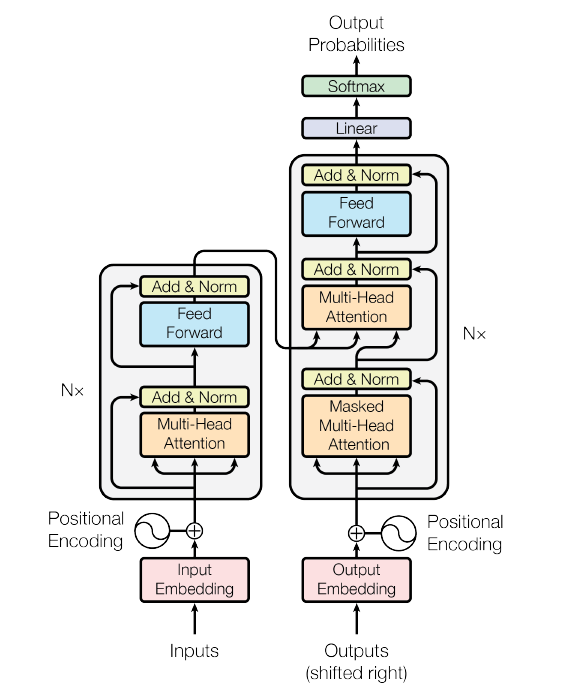
\includegraphics[width=0.5\linewidth]{Figures/fig_17.png}
    \caption{Transformer architecture}
    \label{fig:enter-label}
\end{figure}
The transformer architecture has shown good performances and it is used by one of the most popular llm: GPT-3 \cite{gpt_dugas} but there are other architectures\cite{naveed2023comprehensive}:
\begin{itemize}
    \item \textbf{Encoder-Decoder architecture:} this architecture processes inputs through the encoder and passes the intermediate representation to the decoder to generate the output.\cite{encoder_medium}

    \item \textbf{Casual Decoder architecture:} this architecture does not have an encoder and it uses a decoder in order to generate tokens, each token depends on the previous sequence. \cite{uniteai_decoder}

    \item \textbf{Prefix Decoder architecture:} this architecture is a modification of the causal decoder architecture, it has a bidirectional attention mechanism that can encode the prefix sequence bidirectionally and predict output tokens autoregressively using shared parameters. \cite{llm_labeller}
\end{itemize}
Zero-shot reasoning, made possible by the described architectures, turns large language models into general-purpose tools capable of understanding natural language text and performing tasks ranging from simple text translation to more complex tasks such as question-answering and even code generation. The utility of these models makes them perfect for everyday use, and they find applications in various fields. 

\newpage
\subsection{General purpose large language models}
General purpose large language models are large language models capable of performing a wide variety of tasks and are available online. In this section, I will analyse and discuss the following general purpose large language models.
\begin{itemize}
    \item \textbf{GPT}
    \item \textbf{BERT}

    \item \textbf{PaLM}

    \item \textbf{LLaMA}

    \item \textbf{T5}
    
    \item \textbf{BLOOM}

    \item \textbf{Mistral}
\end{itemize}

\subsubsection{GPT}
The Generative Pretrained Transformer (GPT) is actually the most advanced and powerful large language models available to users. The LLM has been developed by OpenAI and it has been made available to the public in November 2022 in form of a web application called ChatGPT. In two months it gained over than 100 million of users, making it the  fastest-growing consumer software application in history, this massive success it is due to its capacity of understanding user language supporting him in different task.\cite{chatgpt_wiki} 
\begin{figure}[H]
    \centering
    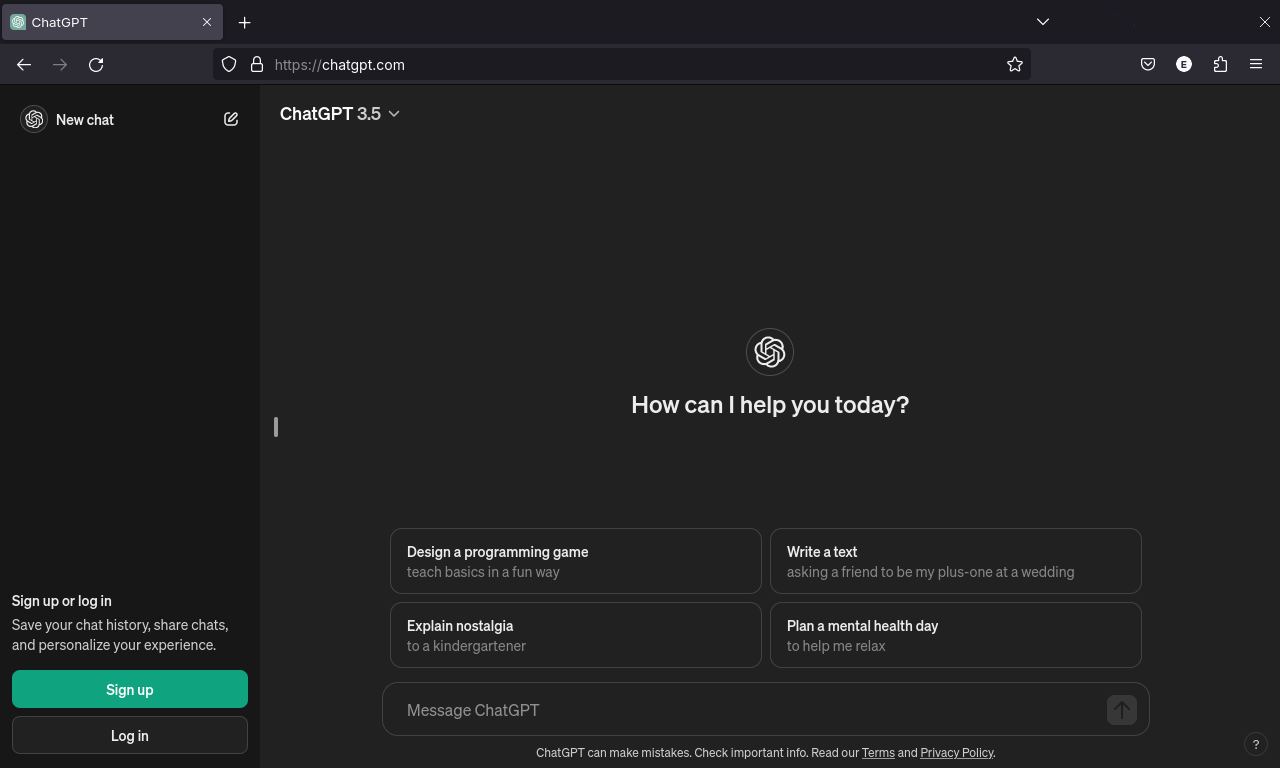
\includegraphics[width=0.9\linewidth]{Figures/fig_18.png}
    \caption{ChatGPT interface}
    \label{fig:enter-label}
\end{figure}
Since its first version, GPT-1 released in 2018, the model represented a step forward in AI development because it was able to comprehend textual material in a more natural manner than before, it had 117 million parameters and it was trained on the BookCorpus dataset. The model was improved in 2019 with the next version: GPT-2 which had 1.5 billions of parameters and it was trained on WebText dataset with 8 millions of documents.\cite{radford2019language} In 2020, OpenAI released GPT-3: this version is more powerful than GPT-2, it is trained over one trillion of internet resources and it has 175 billions of parameters. It is able to perform \textit{in-context learning}, the model recognize pattern in data which is useful when it has few example or just a task description. \cite{journey_gpt}
The latest version of GPT is GPT-4, this large language model is a multimodal model, it can take as input images and text and generate a response. Despite the continuous evolution and the billions of parameters of the model, it is still subject to issues, including hallucinations: it is unable to provide a correct answer and instead outputs false information.\cite{achiam2023gpt}
\subsubsection{BERT}
BERT (Bidirectional Encoder Representations from Transformers) was introduced by Google AI in 2018 and it is described in the paper \textit{"BERT: Pre-training of Deep Bidirectional Transformers for Language Understanding"}.\cite{kenton2019bert} Compared to other models like GPT, BERT is a bidirectional transformer-based model: it takes into account the context on the left and on the right of each word in order to get better understanding of the text. This goal is achieved during the pre-training phase: in the training corpus. tokens are masked randomly allowing the model to predict missing tokens in the text. The pre-training is based on the BookCorpus dataset\cite{bandy2021addressing} and on english Wikipedia. Moreover BERT is able to perform the next sentence prediction nlp task\cite{shi2019next}, predicting a sentence on the basis of the previous sentence.\\
BERT model is used mainly for sentiment analysis and text classification, unlike GPT, it does not have a web interface, but the different versions of BERT are available on Huggingface at this link:\\ https://huggingface.co/docs/transformers/model\_doc/bert.
\subsubsection{PaLM}
In September 2023, Google AI released a more powerful model: PaLM (Pathways Language Model), this model has 540 billions of parameters using a dense decoder-only Transformer model trained with the Pathways system that allows parallel training. \cite{anil2023palm}\cite{barham2022pathways}
PaLM is trained  using a combination of English and multilingual datasets (100 languages) that include high-quality web documents, books, Wikipedia, conversations, and GitHub code, this dataset allows PaLM to do complex reasoning and code generation.\cite{palm2_intro} PaLM is a general purpose large language models but more specialized versions have been developed: 
\begin{itemize}
    \item \textbf{Med-PaLM 2:} this version of PaLM is specifically trained medical text and it is able to give in output medical diagnosis. 
    \item \textbf{Sec-PaLM:} this version of PaLM is applied to cybersecurity, it can analyze and detect malicious scripts that ca be a threat for companies.
\end{itemize}
PaLM represents a significant step forward in large language models and is the direct competitor to GPT. Additionally, it serves as the starting point for an even more powerful multimodal model: Google Gemini, which I will discuss in the following section.
\subsubsection{LLaMA}
LLaMA (Large Language Model Meta AI) is a family of large language models developed by another web giant: META developed introduced in 2023. LLaMA models are based on transformer architecture and, like PaLM, they are trained using different sources, specifically: EnglishCommonCrawl dataset, C4 dataset, Github, Wikipedia, ArXiv and Stack Exchange.  Thanks to the extensive dataset LLaMA models are able to perform common sense reasoning, question-answering, mathematical reasoning, text comprehension and code generation, those abilities have been assessed using zero-shot and few-shot prompting. \cite{touvron2023llama}\\The latest version LLaMA 3 includes over 400 billions of parameters\cite{llama3_intro} and it can be downloaded on huggingface or on the official meta website. More specific LLaMA versions have been developed:
\begin{itemize}
    \item \textbf{Code LLaMA:} Code Llama is a family with the capabilities to accept text prompts and generate and discuss code. The release also includes two other variants (Code Llama Python and Code Llama Instruct) and different sizes.
    \item \textbf{LLaMA Guard:} LLaMA Guard is an LLM-based input-output safeguard model geared towards Human-AI conversation use cases. The model an LLM-based input-output safeguard model geared towards Human-AI conversation use cases.
    \item \textbf{LLaMA 3.2 Vision:} the most advanced version of LLaMA that supports visual prompts.
\end{itemize}
Moreover these version, a version of LLaMA 2 called "LLaMAntino"\cite{basile2023llamantino} that has been created by researchers of the University of Bari ant it is trained on the Italian corpora.
\subsubsection{T5}
T5 (Text-to-Text Transfer Transformer) is an encoder-decoder model, introduced in 2020, pre-trained on a multi-task mixture of unsupervised and supervised tasks\cite{raffel2020exploring} and for which each task is converted into a text-to-text format. The model has been trained on CommonCrawl dataset that includes 750 GB of english text in addition to Wikipedia and RealNews-like dataset.
There are five version of the T5 model:
\begin{enumerate}
    \item \textbf{T5-Base:} 220 millions of parameters.
    \item \textbf{T5-Small:} 60 million of parameters.
    \item \textbf{T5-Large:} 770 million of parameters.
    \item \textbf{T5-3B:} 3 billions of parameters.
    \item \textbf{T5-11B:} 11 billions of parameters.
\end{enumerate}
\begin{figure}[H]
    \centering
    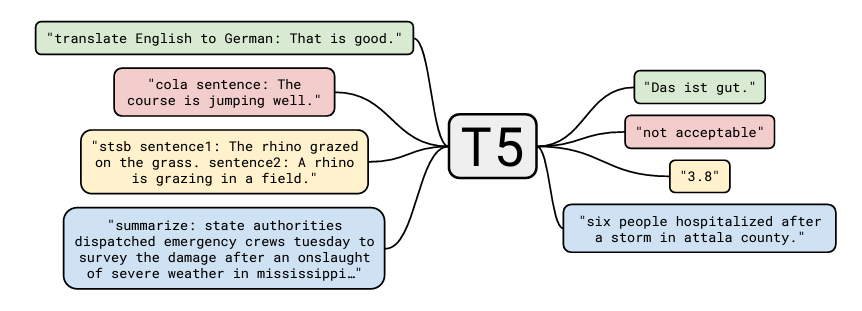
\includegraphics[width=0.8\linewidth]{Figures/fig_19.png}
    \caption{Unified text-to-training}
    \label{fig:enter-label}
\end{figure}
All version of T5 are able to perform different tasks including:\cite{t5_docs}
\begin{itemize}
    \item Text Classification: T5 can classify sentences or documents, it can perform sentiment analysis, grammatical judgments, or assign labels to questions based on their type.

    \item Translation: T5 can translate text between different languages, for example from English to German.

    \item Question Answering: Given a context and a question, the model can provide an accurate answer.

    \item Summarization: T5 can summarize longer documents or articles, generating a brief summary of the content.

    \item Logical Inference: T5 can handle natural language inference tasks where it determines whether one sentence entails, contradicts, or is neutral in relation to another sentence.
\end{itemize}
All the version of T5 models are available on Huggingface at the link:\\
https://huggingface.co/docs/transformers/model\_doc/t5
using the transformers python library.

\subsubsection{BLOOM}
BLOOM (BigScience Large Open-science Open-access Multilingual Language Model) is an open source autoregressive large language model trained to continue text from a prompt on vast amounts of text data using industrial-scale computational resources. In detail the model has 175 billions of parameters and it is trained on a dataset that includes 46 natural languages and 13 programming languages in form of 350 billions of unique tokens.\cite{le2023bloom} BLOOM actually is the biggest and the most powerful open source large language model and it can be used for multilingual content generation, software development and research.\cite{exploring_bloom} The BLOOM llm is available on Huggingface at the link: https://huggingface.co/bigscience/bloom using the transformers python library.
\subsubsection{Mistral}
Mistral is a seven-billion parameters large language models released in September 2023 by the french startup Mistral-AI, the model, like others analyzed, is based on the transformer architecture and it has free versions and premium version available.\cite{jiang2023mistral} Mistral has text and code generation capabilities and it can be used using a web interface available at the link: https://chat.mistral.ai/chat. 
\begin{figure}[H]
    \centering
    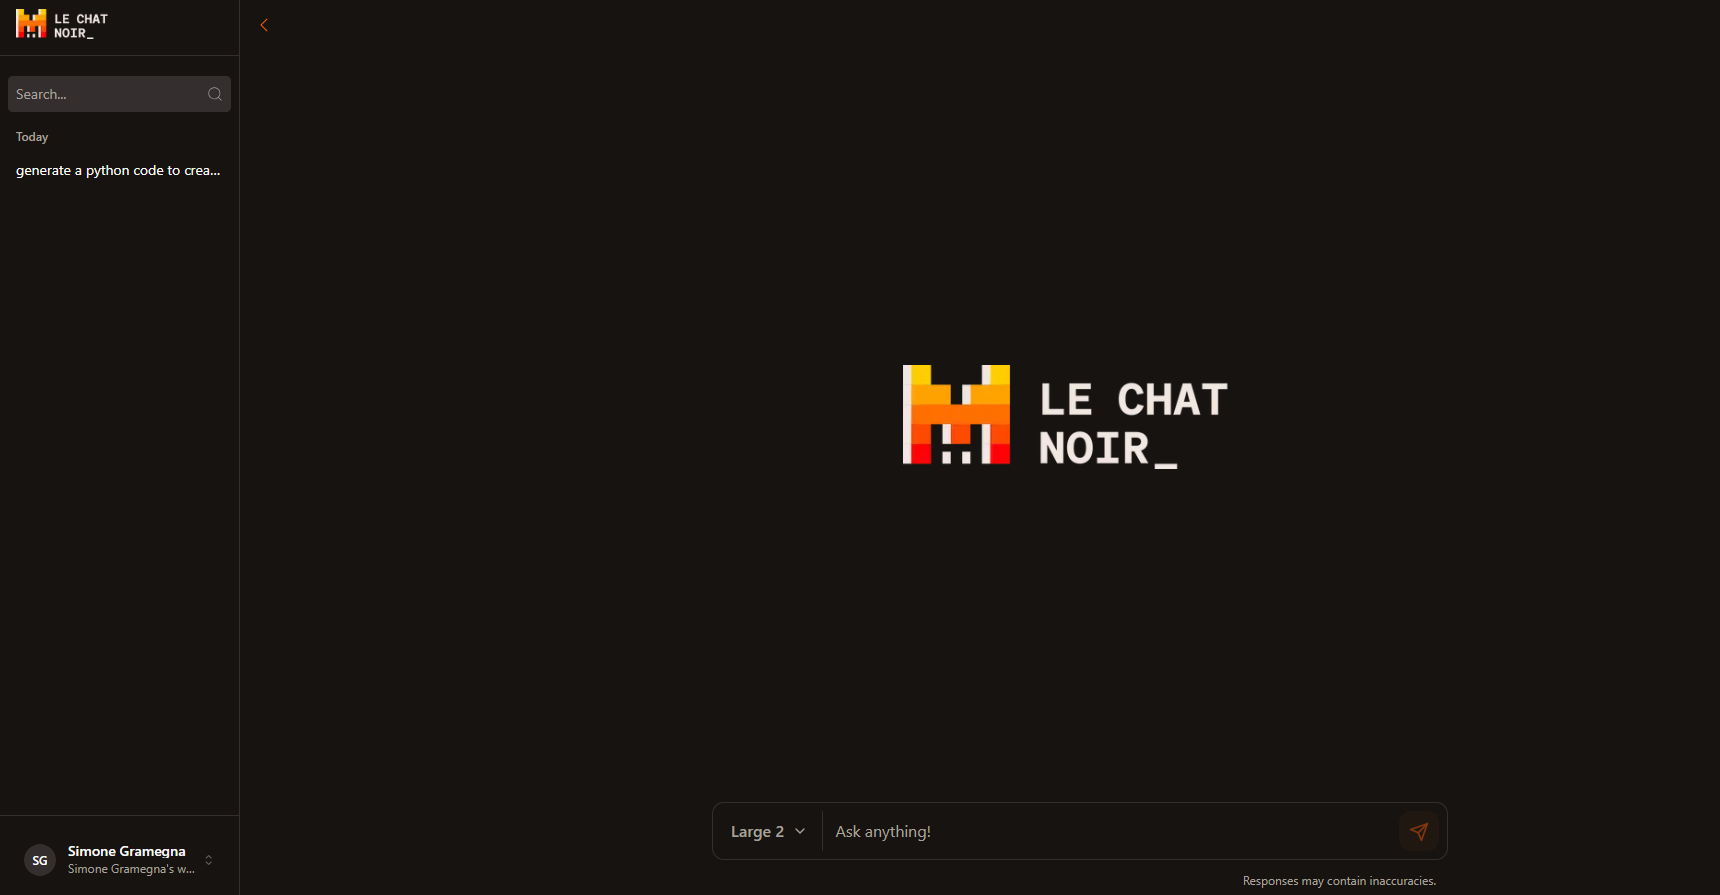
\includegraphics[width=0.9\linewidth]{Figures/fig_20.png}
    \caption{Mistral web interface}
    \label{fig:enter-label}
\end{figure}
Other available versions of Mistral are:
\begin{itemize}
    \item \textbf{Codestral:} Codestral is trained on a dataset of over 80 programming languages, including Python, Java, C, C++, JavaScript, Swift, Fortran and Bash. The model can complete coding functions, write tests, and complete any partial code using a fill-in-the-middle mechanism. 
    \item \textbf{Mistral Nemo:} Mistal Nemo is a more advanced version of Mistral 7B, created in collaboration with NVDIA, it has 12 billions of parameters.
    \item \textbf{Pixtral:} Pixtral is a multimodal large language model created starting from Mistral Nemo, the model can take in input text and images.
\end{itemize}
The presented large language models are the main general-purpose LLMs available to the public; some, like GPT, PaLM, or Mistral, offer a web interface and are generally based on the transformer architecture, which enables natural language processing and text generation. In the following section, I will discuss multimodal large language models (MLLMs), which are large language models capable of accepting and processing data not only in text form but also as files and images.

\newpage
\subsection{Multimodal large language models}
\subsubsection{Introduction to MLLMs}
The evolution of large language models is represented by multimodal large language models, which are capable of processing information in various forms: text, images, audio, video, documents. At the core of these models’ functionality there is a complex Transformer architecture where images, audio, and video are transformed into embeddings, that are multidimensional vector representations. Processing these embeddings through a multi-layered network generates an output in the form of text or an image\cite{wadekar2024evolution} as we can see in the figure below: 
\begin{figure}[H]
    \centering
    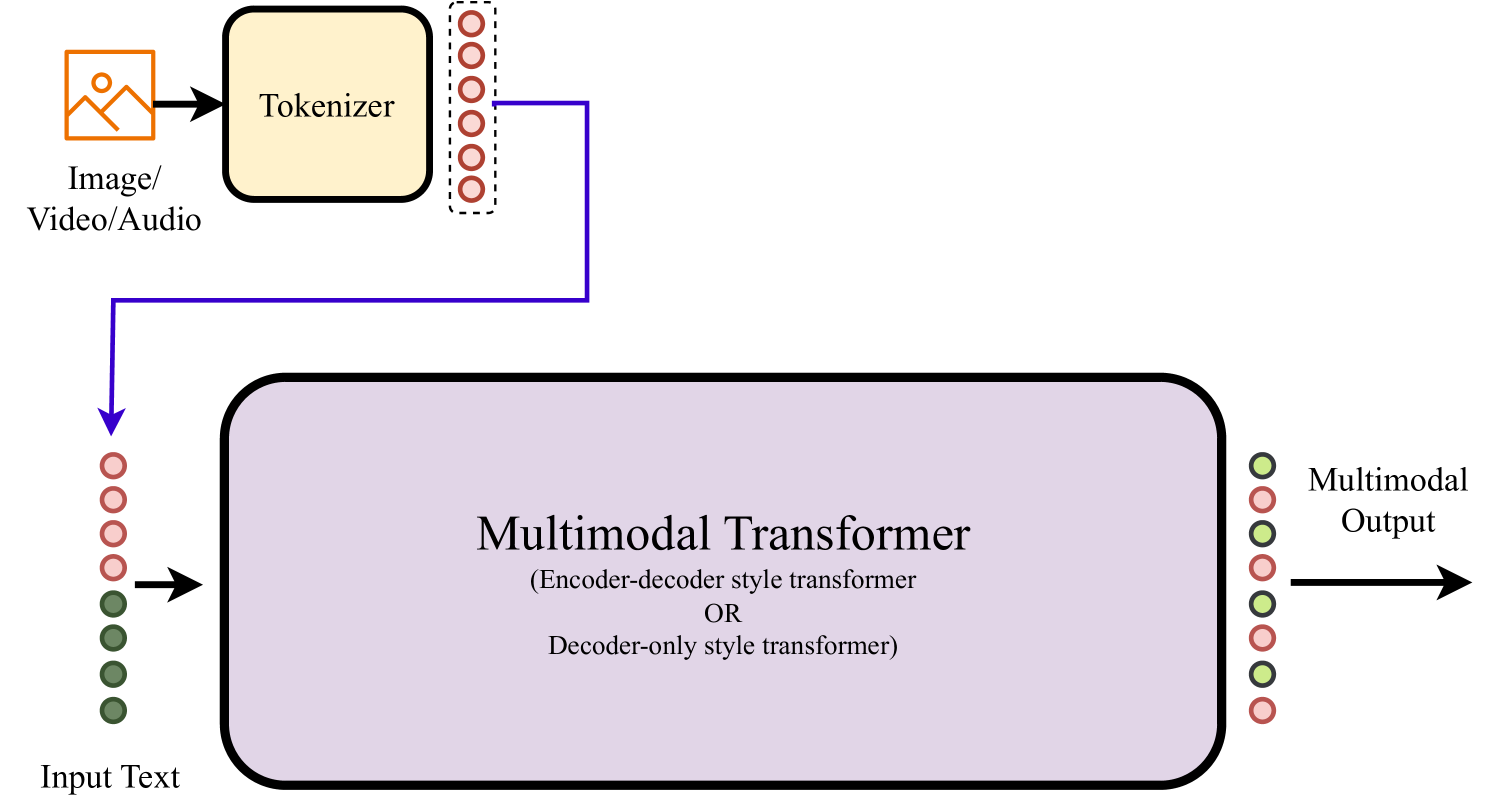
\includegraphics[width=0.9\linewidth]{Figures/fig_21.png}
    \caption{Example of multimodal transformer architecture}
    \label{fig:enter-label}
\end{figure}
This architecture in multimodal large language models is applied in order to do two main tasks:
\begin{enumerate}
    \item \textbf{Image-To-Text:} This task consists of assigning a textual description to an image by recognizing the elements present within it.


    \item \textbf{Text-To-Image:} This task consists in generating an image, given a text by recognizing the meaning and the semantics of the words.
\end{enumerate}
There are several multimodal large language models capable of solving these tasks, representing evolutions of large language models already introduced and described. The main MLLMs we will cover are the following:

\begin{itemize}
    \item \textbf{GPT-4}

    \item \textbf{Google Gemini} 

    \item \textbf{GLaMM}

    \item \textbf{BLIP-2}
\end{itemize}

\subsubsection{GPT-4}
GPT-4 is the latest version of the most popular large language model: GPT. Released in March 2023, it became available to premium users of the ChatGPT platform in three distinct versions: GPT-4, GPT-4 Turbo, and GPT-4o (omni). These versions represent an evolution of the GPT-3 model, enhancing performance, response speed, and processing a higher number of tokens per minute.\cite{insights_gpt4} The multimodal version of GPT-4, known as GPT-4o where the "o" stands for "omni," highlighting the "omniscience" of this model is capable of:
\begin{itemize}
    \item Real-time voice communication: GPT-4o is able to engage in real-time voice conversations, understanding spoken input and generating natural-sounding voice responses.

    \item Real-time vision: GPT-4o is able to process and understand vision data like images and video and their semantics. The model can generate an image starting from text and applying styles or generating descriptions of an image.

    \item Code Reading Through Vision: this feature is very useful for developers, given a screen of an IDE like Eclipse or Visual studio code. GPT-4o can read and understand the code inside the image, giving useful responses to developers.

    \item Data and Chart Reading: GPT-4o can read and interpret data in forms of charts and graphs, giving useful insights.
\end{itemize}
These features make GPT-4o a versatile and powerful tool applicable in many sectors, with particular emphasis on programming and data analysis. Details regarding the dataset, number of parameters, and training technique are not disclosed for competitive reasons.
\subsubsection{Google Gemini}
The latest evolution of Google's large language models is Gemini, this model has been introduced in 2023 and it is the evolution of Bard: the chatbot based on PaLM which I discussed in the previous section. Google Gemini, like GPT-4, is not only capable of generating and understanding text but can also interpret images, videos, and audio, accepting multimodal prompts.\cite{gemini_introduction}
Gemini has proven to be superior to its rival GPT-4 on various benchmarks, achieving results of up to 90\% accuracy.
\subsubsection{GLaMM}
GLaMM (Grounding LLM) is a multimodal large language model that integrates natural language with object segmentation masks in images, combining scene-level, region-level, and pixel-level understanding. 
The model uses an auto-encoder to process images and an LLM to understand natural language. The encoder is based on ViT-H/14 from CLIP and there are a grounding image encoder, a pixel decoder, and a region encoder inspired by GPT4Rol. The LLM is based on Vicuna with 7 billion parameters, and the vision-language and language-prompt projection layers are implemented using a 2-layer MLP activated with GELU. \cite{rasheed2024glamm}
\begin{figure}[H]
    \centering
    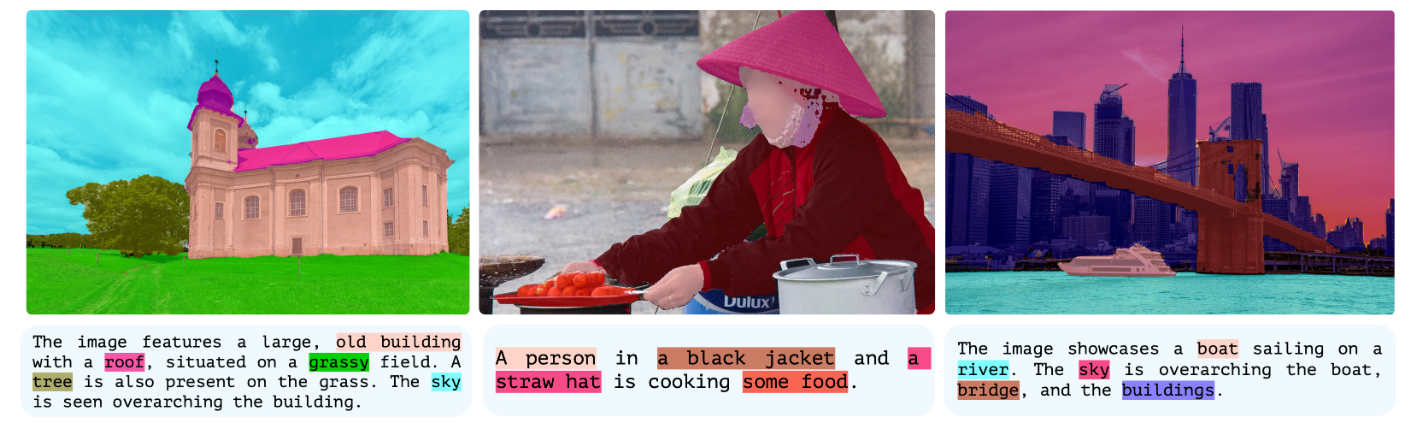
\includegraphics[width=0.9\linewidth]{Figures/fig_23.png}
    \caption{GLaMM object segmentation}
    \label{fig:enter-label}
\end{figure}
The source code is available on the official GitHub repository:\\ \href{https://github.com/mbzuai-oryx/groundingLMM}{https://github.com/mbzuai-oryx/groundingLMM}

\subsubsection{BLIP-2}
BLIP (Bootstrapping Language-Image Pre-training) is a multimodal large language model developed in 2023 by Salesforce: an IT company in the filed of CRMs.
The model has 188 millions of parameters and the architecture is composed by three principal components:
\begin{enumerate}
    \item Image encoder: There is a vision encoder ViT-L/14.

    \item Q-Former: The query transformer (Q-Former) matches the embedding representation of the image with the text.

    \item Large Language Model: The llm is based on T5 and gets the input from the Q-Former in order to create image descriptions.
\end{enumerate}
BLIP-2 architecture is designed to generate captions starting from images, this task is called vision-to-language generation. This task is performed in a zero-shot setting: the model has no similar example to the image. Another task that the model can perform is visual question answering (VQA), answering questions about image content on which it can reason about interpreting complex scenes and making inferences about them. 
\begin{figure}[H]
    \centering
    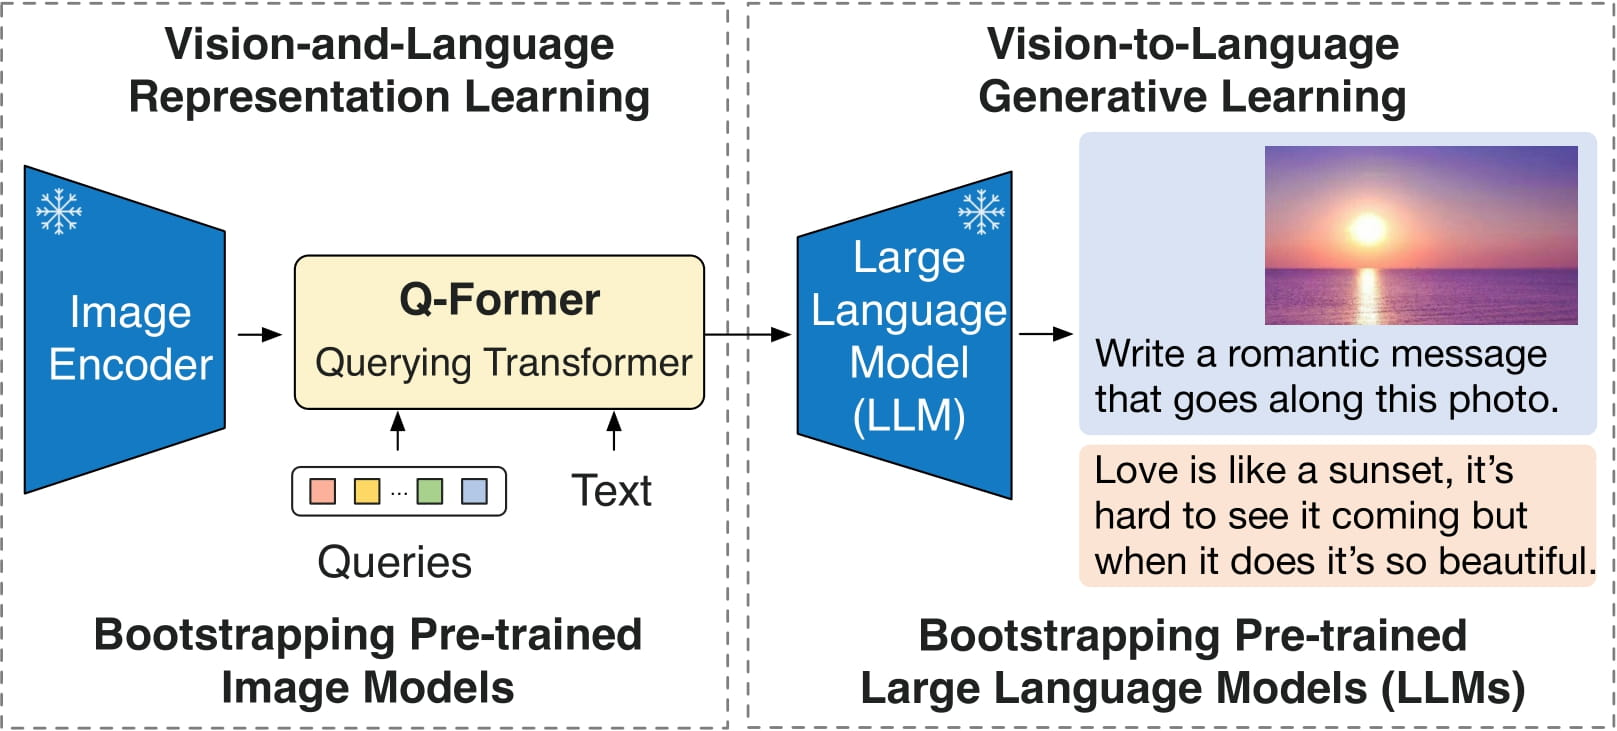
\includegraphics[width=0.7\linewidth]{Figures/fig_24.jpg}
    \caption{BLIP-2 architecture}
    \label{fig:enter-label}
\end{figure}
\newpage
\section{Prompt engineering}
\subsection{What is prompt engineering?}
At the core of interaction with large language models are prompts, a prompt is an instruction written in natural language given as input to a large language model to generate a response or action.\cite{llm_prompt}
A prompt can be written without a criteria or following specific prompting techniques that describe the structure, the application of those techniques iteratively is the prompt engineering\cite{schulhoff2024prompt}, in this process there is the modification of the structure in order to get better and more accurate results from the model. A prompt can be structured in different ways, the first way is writing the instructions and include a direct question like:
\begin{lstlisting}
How should I write my college admission essay? Give me suggestions about the different sections I
should include, what tone I should use, and what expressions I should avoid.   
\end{lstlisting}

The second way is just the specification of the input without any question like:
\begin{lstlisting}
Tell me five good books to read. 
\end{lstlisting}
In some cases it useful to provide context and examples in the prompt or specify the output formatting because basically the output is plain text for example:
\begin{lstlisting}
Tell me five good books to read.
Give me the list into a csv.
\end{lstlisting}
We can see a prompt like a mathematical function that takes in input a text and gives an output $ f(x) = y$ in which $f()$ is the template applied to the text of the problem, for example if we want to translate a phrase in english: 
\begin{lstlisting}
Translate {X} in english
\end{lstlisting}
This is just a simple technique in which there is the manual creation of the template but there are in literature more complex techniques that we are going to discuss.
\subsection{Prompt engineering techniques}
Prompt engineering techniques involve structuring a prompt in a specific way according to a particular strategy in order to obtain more accurate responses and a better understanding of the problem to be solved by the model. The first and simplest technique is the \textbf{Zero-shot prompting} in which no example is provided, and the large language model has no prior knowledge of the context, generating the output based solely on the given input prompt. An example is the following: 
\begin{lstlisting}
Classify the text into neutral, negative or positive. 
Text: I think the vacation is okay.
Sentiment:   
\end{lstlisting}
In \textbf{Few-shot prompting}, on the other hand, the input prompt provided to the large language model includes a few examples, with the aim of not only achieving a better understanding of the context (something that was not possible with zero-shot prompting) but also obtaining improved performance, as we can see in the following example:
\begin{lstlisting}
Task: Translate the following sentences from italian to english.

Example "Oggi il tempo e' bello" output: "The weather is nice today"

input: "Mi piace leggere libri" // output: I love reading books
\end{lstlisting}
The two techniques are thus based on a single prompt, but we can use multiple prompts, in the multi-prompt learning  
we can follow a reasoning process and in this sense the main technique is \textbf{Chain-of-Thought (CoT) Prompting}, where logical reasoning is done step by step to achieve more structured and accurate responses. An example is the following:
\begin{lstlisting}
Q: Roger has 5 tennis balls. He buys 2 more cans of tennis balls. Each can has 3 tennis balls. How many tennis balls does he have now? 
A: Roger started with 5 balls. 2 cans of 3 tennis balls each is 6 tennis balls. 5 + 6 = 11. The answer is 11.  
Q: The cafeteria had 23 apples. If they used 20 to make lunch and bought 6 more, how many apples do they have?

Model output: The cafeteria had 23 apples originally. They used 20 to make lunch. So they had 23 -  20 = 3.  They bought 6 more apples, so they have 3 + 6 = 9. The answer is 9.   
\end{lstlisting}
The main issue with this technique is the manual intervention required, as the user must manually provide the reasoning that the large language model will follow. To address this problem, a variant called \textbf{Automatic Chain-of-Thought (Auto-CoT) Prompting} was introduced. Instead of manually providing the reasoning chain, the prompt includes a simple phrase, "Let's think step-by-step," to automatically generate multiple reasoning chains.\\
Both CoT and Auto-CoT follow a single reasoning path but we can generate multiple reasoning paths and choose the best answer, this is the basis of the \textbf{Self-consistency prompting}\cite{wang2022self}. Multiple reasoning paths are created using chain of thought prompting and then evaluating responses.\\
Another technique that generate mutliple resoning paths is the \textbf{Thread of Thought (ThoT)}
prompting technique. In practice, a tree-of-thought is automatically generated, and each step of the reasoning process is evaluated automatically. Additionally, by combining graph search algorithms such as BFS (Breadth-First Search) and DFS (Depth-First Search), the ability to evaluate different reasoning paths is improved.
\begin{figure}[H]
    \centering
    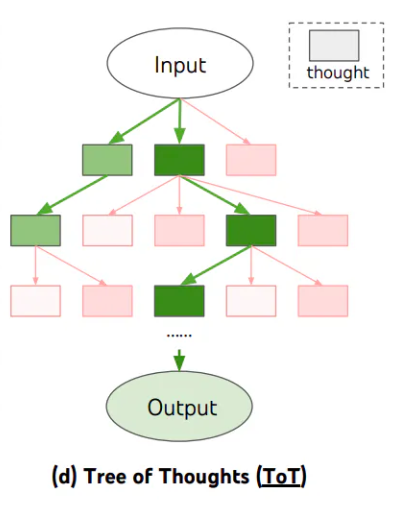
\includegraphics[width=0.4\linewidth, height=7cm]{Figures/fig_6.png}
    \caption{Thread of Thought (ThoT) Prompting}
    \label{fig:enter-label}
\end{figure}
It is possible to adapt the large language model to the different reasoning task using the \textbf{Active prompting} that enhances performance introducing a mechanism for determining the most impactful questions for annotation. Starting from a set of questions $Q = \{q_1, q_2, ..., q_n\}$ the goal is to annotate the answers ($a_i$) obtained with intermediate steps ($c_i$):\\ $E = \{(q_1, c_1, a_1), (q_2, c_2, a_2) ..., (q_n, c_n, a_n)\}$ there is the measurement of the disagreement of the answers, the entropy and the variance. Once the best k-questions with their respective answers are selected, self-consistency is applied (a technique that generates multiple outputs from a single prompt) \cite{wang2022self}, and finally, the most relevant answers are chosen.\\
Those technique involving multiple prompts are useful in order to decide the best reasoning strategy but we can also decide not to use any complex reasoning but a more simple strategy that can involve the ensembling, the augmentation, the composition or the decomposition of a single prompt.\cite{liu2023pre} In \textbf{prompt ensembling} there is the combination of different prompt on the same subject to get the response for example:
\begin{lstlisting}
PR1: China's capital is [X]
PR2: [X] is capital of China
PR3: The capital of China is [X]
\end{lstlisting}
To choose the response, we can apply several strategies, including majority voting, weighted voting ecc.. 
In \textbf{prompt augmentation} there are additional examples providing the model an example of response (this is similar to few-shot prompting) for example:
\begin{lstlisting}
Main prompt: 6 + 8 = [X]
PR1: 1 + 1 = 2
PR2: 2 + 5 = 7
\end{lstlisting}
In \textbf{prompt composition} there is a composition of two or more subprompts in order to get the final prompt in contrast in \textbf{prompt decomposition} one main prompt is decomposed in two or more smaller subprompts.
In large language models, there is a significant issue that leads to incorrect responses, known as the problem of hallucinations. We refer to hallucination, in the context of LLMs, when there is the generation of texts or responses that are grammatically and syntactically correct but deviate from the given inputs or do not align with factual accuracy. \cite{ye2023cognitive} Prompt engineering techniques can help reduce this phenomenon,the main technique is \textbf{Retrieval Augmented Generation (RAG)}. In this approach, starting from an input, a knowledge base of sources (web pages, articles, etc.) is created, and the text from these sources is incorporated into the subsequent input, providing context and generating more accurate and reliable responses. Another technique, that combines reasoning and acting with LLMs, is the \textbf{ReAct Prompting}. A ReAct prompt consists of few-shot task-solving trajectories, with human-written text reasoning traces and actions, as well as environment observations in response to actions \cite{react_llm} an example, provided by the authors is the following: 
\begin{figure}[H]
    \centering
    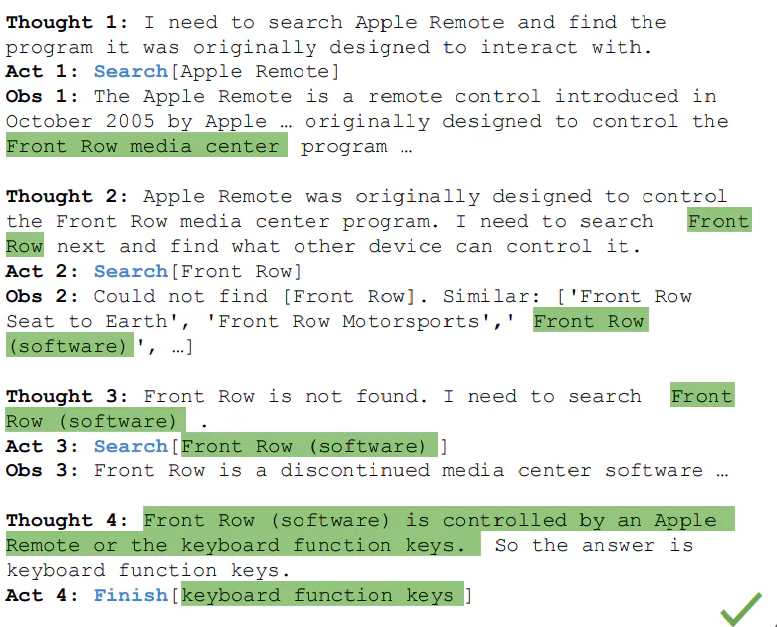
\includegraphics[width=0.7\linewidth]{Figures/fig_7.png}
    \caption{ReAct Prompting}
    \label{fig:enter-label}
\end{figure}
The improvement in performance and accuracy of the responses obtained from the large language model can also be achieved by incorporating the user's emotions into the prompt, known as \textbf{Emotion Prompting}.
Incorporating emotions can be useful in tasks such as sentiment analysis of a sentence, but this is not the case for code generation, for which various prompt engineering techniques have been introduced. \\
An evolution of the previously described Chain-of-Thoughts is \textbf{Program of Thoughts (PoT) Prompting} \cite{chen2022program}, where the large language model is given a prompt containing intermediate steps that include mathematical expressions or source code, as we can see in the following figure:
\begin{figure}[H]
    \centering
    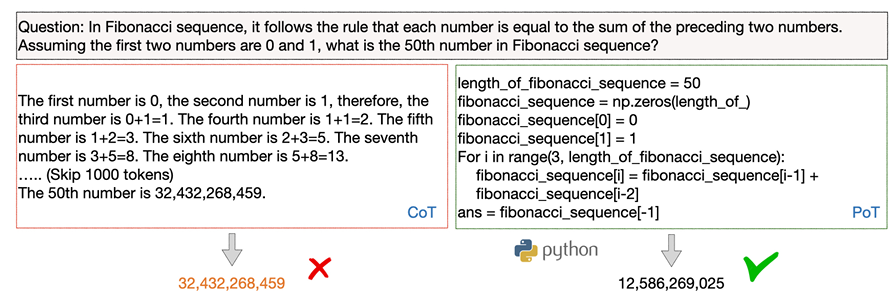
\includegraphics[width=0.7\linewidth]{Figures/fig_8.png}
    \caption{Program of Thoughts (PoT) Prompting}
    \label{fig:enter-label}
\end{figure}
Another approach is the \textbf{Scratchpad Prompting} in which there is the generation of an arbitrary sequence of intermediate tokens before providing the final answer. The sequence is given in a tag called "scratch"\cite{scratch}\cite{nye2021show} in which the user writes intermediate steps useful to the large language model as shown below: 
\begin{lstlisting}
<scratch>
2 9 + 5 7 ,  C: 0
2 + 5 , 6 C: 1    # added 9 + 7 = 6 carry 1
, 8 6 C: 0        # added 2 + 5 + 1 = 8 carry 0
0 8 6
</scratch>
8 6
\end{lstlisting}
In the example above we teach the LLM the addition of two numbers. \\
The techniques illustrated aim to reduce calculation and output generation errors produced by large language models through examples or reasoning sequences provided manually. The \textbf{Rephrase and Respond (RaR) Prompting}\cite{deng2023rephrase} technique automatically allows for the correction and improvement of the LLM's response through the prompt:
\begin{lstlisting}
"{question}" Rephrase and expand the question, and respond.
\end{lstlisting}
This approach has four main advantages:
\begin{enumerate}
    \item It lets the LLM self-improve the prompts while maintaining the context of the original query.

    \item It allows better aligning the human’s intended query with LLM’s preferred style of question.

    \item It expands the LLM’s thought process and adding a step that will not naturally appear when using CoT.

    \item It provides an approach for humans to interpret how LLMs understand the questions.
\end{enumerate}
Another technique to obtain more accurate and comprehensive responses is the \textbf{Take a Step Back Prompting}\cite{zheng2023take}, which consists of two steps. The first step involves inputting a specific question, and subsequently (step-back) inputting a more abstract, high-level question related to the task, as shown in the following figure:
\begin{figure}[H]
    \centering
    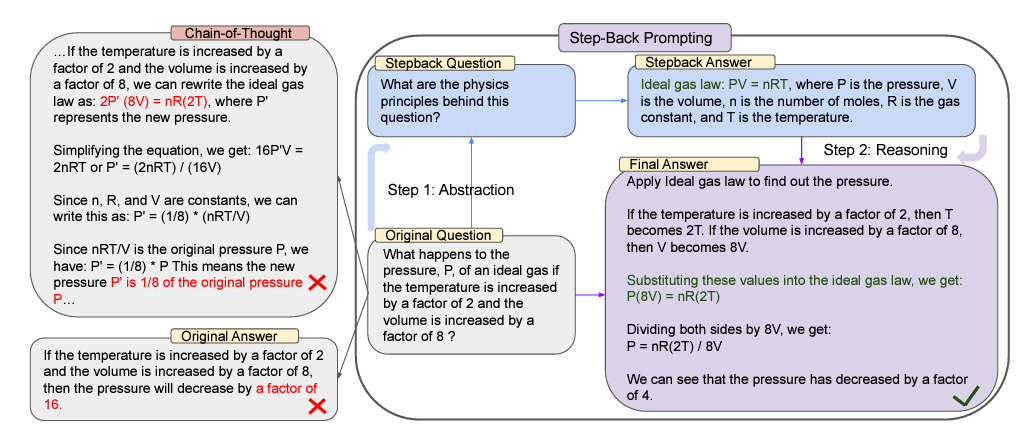
\includegraphics[width=0.9\linewidth]{Figures/fig_9.png}
    \caption{Take a Step Back Prompting}
    \label{fig:enter-label}
\end{figure}

\subsection{Prompt engineering in multimodal LLMs}
State-of-the-art prompt engineering techniques aim, when given as input to a large language model, to generate text. The most recent advancements in technology allow for incorporating images into the prompt or generating images using multimodal large language models. 
Main tasks involving multimodal large language models are:
\begin{itemize}
    \item Image generation
    \item Image classification
    \item Image editing
    \item Image classification
\end{itemize}


A preliminary approach to image classification is the use of two techniques, namely zero-shot prompting and few-shot prompting. \cite{chen2023unleashing} In zero-shot prompting for image generation, no input examples are provided, but only the instruction to be executed, for example:
\begin{lstlisting}
Classify the follwing image: [image.png]
\end{lstlisting}
In few-shot prompting examples are provided to the model, for example:
\begin{lstlisting}
Given: [image1.png], [image2.png], [image3.png], classify the following image: [image.png]
\end{lstlisting}
Zero-shot prompting and few-shot prompting can be also used in image generation, this task is more complex and it can be useful to incorporate user feedback that helps improve the generated image. An example is drawing a stick figure using letters of the alphabet \cite{proptingguide_image}, where the process starts from an initial prompt, such as:
\begin{lstlisting}
Produce TikZ code that draws a person composed from letters in the alphabet. The arms and torso can be the letter Y, the face can be the letter O (add some facial features) and the legs can be the legs of the letter H. Feel free to add other features.    
\end{lstlisting}
The generated image is refined by adding details: 
\begin{lstlisting}
- The torso is a bit too long, the arms are too short 
  and it looks like the right arm is carrying the face instead of the face being right above the torso. Could you correct this please? 

- Please add a shirt and pants.
\end{lstlisting}
As we can see in the following example, where the latest version of ChatGPT, GPT4, has been applied:
\begin{figure}[H]
    \centering
    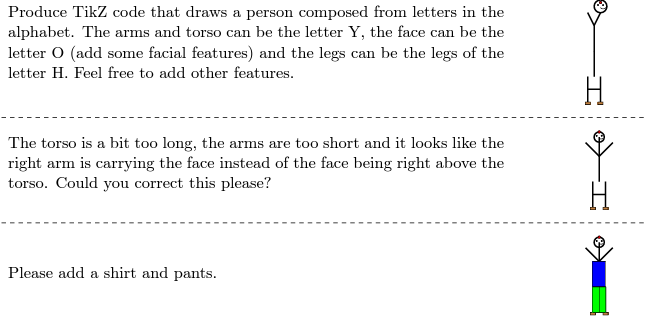
\includegraphics[width=0.8\linewidth]{Figures/fig_10.png}
    \caption{Drawing using GPT4}
\end{figure}
In image generation the characteristics of an image can be specified not only using user feedback but also using \textbf{style modifiers}. Style modifiers are  descriptors that consistently produce certain styles, for example: "tinted red", "made of glass", and combining those together they produce a more specific style. \cite{lp_style} 
For example we want to generate using DALL-E a picture of a pyramid, the first picture is generated without using any modifier:
\begin{figure}[H]
    \centering
    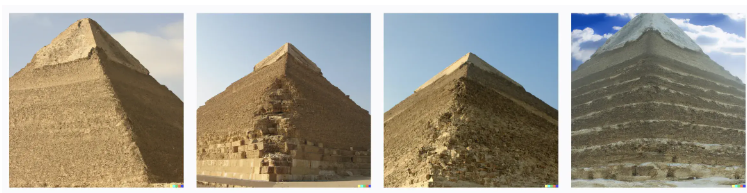
\includegraphics[width=0.9\linewidth]{Figures/fig_11.png}
    \caption{Pyramid picture with no modifiers}
    \label{fig:enter-label}
\end{figure}
The second picture is generated using the prompt with three modifiers: \textit{A pyramid made of glass, rendered in Unity and tinted red} getting the following result:
\begin{figure}[H]
    \centering
    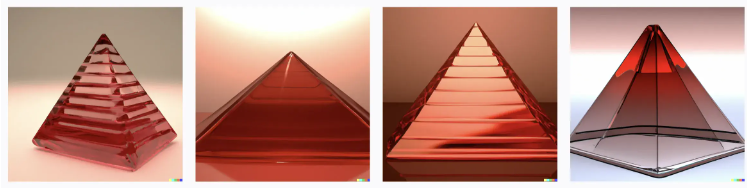
\includegraphics[width=0.9\linewidth]{Figures/fig_12.png}
    \caption{Pyramid picture with modifiers}
    \label{fig:enter-label}
\end{figure}
In the prompt, in order to improve quality, we can add generic adjectives like: \textit{"amazing"}, \textit{"good"}, \textit{"beautiful"} that are called \textbf{quality boosters}. \cite{oppenlaender2023taxonomy} 
The Latin motto \textit{"repetita iuvant"} that means that repeating words is useful can be applied in a certain sense in a prompt for image generation. In the \textbf{repetition technique} if we want to give more importance to some adjective instead of another it is possible to repeat more times the word, giving to it emphasis. For example if we want to generate an image of a waterfall for example but we want to emphasise the beauty of the picture we can use this following prompt:
\begin{lstlisting}
A very very very very very beautiful painting of a mountain next to a waterfall
\end{lstlisting}
In this case the word "very" is repeated five times in order to give more importance to the adjective beautiful.\\
Repeating terms in a prompt can be weird and inaccurate, it is possible to use \textbf{weighted terms technique}\cite{weighted_terms} in which a term has a numerical value (positive or negative) that corresponds to the weight, the importance of that term. For example if we want to generate a picture of a mountain without trees, we use this prompt:
\begin{lstlisting}
mountain | tree:-10.
\end{lstlisting}
in which the tree has negative weight and it doesn't have importance getting this result:
\begin{figure}[H]
    \centering
    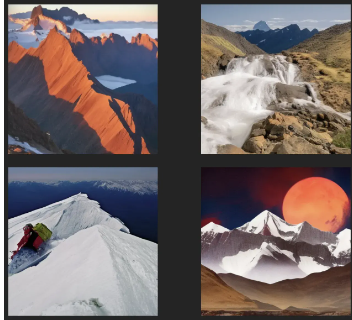
\includegraphics[width=0.5\linewidth]{Figures/fig_15.png}
    \caption{Weighted terms image}
    \label{fig:enter-label}
\end{figure}

Another approach in image generation is negative prompting, negative prompts allow users to exclude unwanted features and enhance the quality output.
Negative prompts are complementary to  positive prompts which describe what the user wants, including the main subject and how it should look.\cite{medium_negative}
For example, we want to generate using a diffusion model a portrait of a man without mustache so the prompt is:
\begin{lstlisting}
- Positive prompt: Portrait photo of a man.
- Negative prompt: Mustache
\end{lstlisting}
Negative prompts can be applied on any image feature like: colors, lighting problems, unwanted elements, image quality and style.\\
Multimodal large language models can be used not only to generate photorealistic images but also artistic images following the style of a particular artist or artistic movement, as discussed in the paper \textit{Design Guidelines for Prompt Engineering Text-to-Image Generative Models} \cite{liu2022design}. The study using the CLIP model generates images in 51 artistic style using the following prompt:
\begin{lstlisting}
SUBJECT in the style of STYLE
\end{lstlisting}
and its permutations like:
\begin{itemize}
    \item A MEDIUM of SUBJECT in the STYLE style - a painting of love in the abstract style

    \item A STYLE MEDIUM of a SUBJECT - an abstract painting of love

    \item SUBJECT STYLE - love abstract art

    \item SUBJECT.STYLE - love.abstract art

    \item SUBJECT in the STYLE style - love painted in the abstract art style

    \item SUBJECT VERB in the STYLE style - love painted in the abstract style

    \item SUBJECT made/done/verb in the STYLE art style - love done in the abstract art style

    \item SUBJECT with a STYLE style - love with an abstract art style
\end{itemize}
A total of 1,296 were generated with 144 permutations for each of the 9 selected subjects: love, hate, happiness, sadness, man, woman, tree, river and dog. The applied prompting technique has produced interesting results that can be qualitatively evaluated and still reflect the desired styles provided as input in the prompt.\\
In the techniques previously described, the prompt consists only of text, but in some models, it is possible to integrate one or more images along with the text, not only to generate images but also to obtain responses related to input images. The \textbf{Multimodal Chain-of-Thought} prompting technique\cite{zhang2023multimodal} is a variation of the Chain-of-Thought technique (CoT), this technique in Multi-CoT is enhanced by incorporating in the prompt text and visual inputs. The technique consists in two stages:
\begin{enumerate}
    \item Rationale generation: the model processes the multimodal inputs in order to generate an intermediate reasoning chain (rationale). The rationale explains the logical steps required to arrive at the final answer, using both textual and visual content as context.

    \item Answer inference: the generate rationale is combined with the original input and used by the model to infer the final answer.
\end{enumerate}
as we can see in the figure below:
\begin{figure}[H]
    \centering
    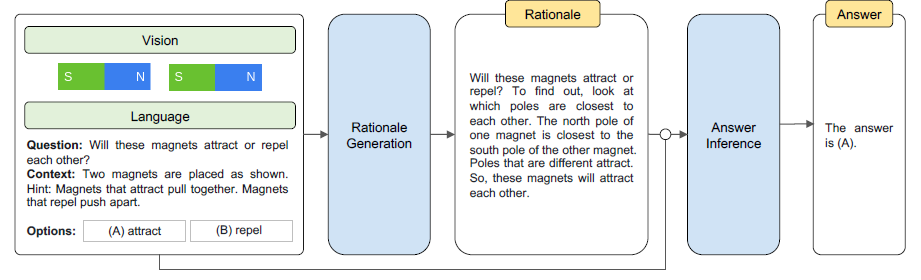
\includegraphics[width=0.9\linewidth]{Figures/fig_16.png}
    \caption{Multimodal Chain-of-Thought}
    \label{fig:enter-label}
\end{figure}
The technique has been tested on T5, UnifiedQA and FLAN-Alpaca and it has a good accuracy averaging around 85\%.\\
Similar to the multimodal chain-of-thought, the \textbf{Chain of Images (CoI)} prompting technique \cite{meng2023chain} generates a series of images as intermediate representations in order to solve problems starting from a textual prompt. Although the technique is innovative as it uses images instead of text, it is not applicable to large language models outside the SyMLLM framework, which is capable of reasoning using this technique. \\\\ 

\chapter{Ontology design}
This chapter details the design phase of the prompt engineering ontology, starting from an ontology engineering methodology chosen based on specific motivations.\\
In the background chapter, in particular in the sections \textit{"Ontology engineering methodologies"} and \textit{"LOT methodologies"} the main state-of-art ontology engineering methodologies have been illustrated:
\begin{itemize}
    \item \textbf{Methontology}
    \item \textbf{NeOn}
    \item \textbf{eXtreme design}
    \item \textbf{LOT - Linked Open Terms}
\end{itemize}
Additionally, in the section \textit{"Ontology engineering using large language models"} two experimental methodologies were analysed, including \textbf{NeOnGPT}, which employs large language models. Each methodology has its features and defines a workflow in order to develop successfully an ontology. The choice of the methodology to follow during the design and development phase is based on an analysis of the pros and cons of each, considering not only their features but also the available resources and the related projects provided by each one. \\
In the state-of-the-art study, the most recent and comprehensive methodology is the \textbf{LOT methodology}, which I have decided to choose and according to which the development of the prompt engineering ontology will be carried out. Compared to other methodologies analysed, this is a recent methodology, introduced in 2022, and has been used in various projects such as the 'Ciudades Abiertas' project \cite{ciudad} for the construction of a set of ontologies used for sharing open data, and the BIMERR project \cite{bimerr}, in which ontologies for sustainable construction were developed \cite{bountouni2021bimerr}, among many others available on the LOT methodology website: \href{https://lot.linkeddata.es/}{https://lot.linkeddata.es/}. The LOT methodology has not only been successfully applied in industrial projects but also in the development of various research ontologies, as seen in the background chapter, as it provides a straightforward and iterative method for designing and developing ontologies. Another reason for choosing this methodology is its ease of learning, as it is inspired by the agile methodology in software development. Moreover, the Linked Open Terms project not only provides very useful examples of ontologies to draw inspiration from but also offers a Github repository \cite{lot_github} with all the necessary resources to be used in the specification of requirements. This last aspect is very important because the main drawback of the other methodologies analysed is the lack of concrete guidelines and the relevant tools to use, tools that, when mentioned, are often obsolete or inaccessible. This complicates the work of a developer who is approaching ontology engineering for the first time, as he needs to understand the fundamentals of the methodology but also figures out which development, validation, and testing software to use. The LOT methodology, thanks not only to the numerous available resources but also to the clear and precise description of the method and the recent tools to be used, resolves these issues and simplifies the developer's work. The LOT methodology has an inherently iterative nature and is oriented towards the publication of ontologies according to the FAIR principles \cite{fair_eu} (Findable, Accessible, Interoperable, Reusable) including specific recommendations, tips and potential
tools that can be helpful to ontology developers moreover the methodology extends the state-of-art methodologies like NeOn and Methontology with a modern approach.
The LOT methodology was preferred over recently introduced techniques that involve the use of large language models in the construction of ontologies and knowledge graphs, such as NeOnGPT. Although these techniques automate the work of the ontology engineer by using large language models, they are computationally expensive and require numerous checks to verify the syntactic and semantic correctness of the produced artifact. Another downside is the lack of actual ontology projects implemented using large language models, as these are very recent techniques that have not been tested on real projects but only on experimental cases.\\
In the following sections, the application of the LOT methodology to the design and implementation of the prompt engineering ontology will be described, following the workflow outlined and described in the background chapter.

\newpage

\section{Ontology requirements specification}
The LOT methodology includes six mandatory phases (plus one optional) in the ontology requirements specification. At the end of each phase, a document is produced containing the analysed aspect of the specifications, as shown in the following figure:
\begin{figure}[H]
    \centering
    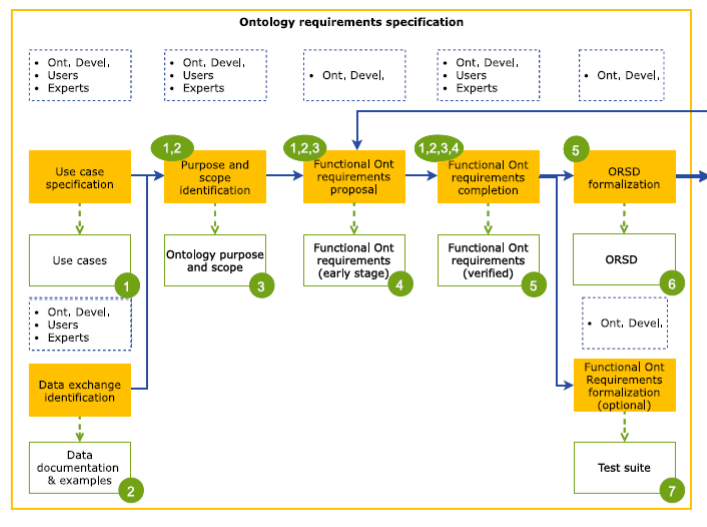
\includegraphics[width=0.9\linewidth]{Figures/fig_13.PNG}
    \caption{Ontology requirements specification workflow}
    \label{fig:enter-label}
\end{figure}
In detail the phases are the following:
\begin{enumerate}
    \item Use case specification
    \item Data exchange identification
    \item Purpose and scope identification
    \item Functional ontology requirements proposal
    \item Functional ontology requirements completion
    \item ORSD formalization 
    \item Functional ontology requirements formalization (optional)
\end{enumerate}

\section{Use case specification}
The first step in the design of the prompt engineering ontology is the use case specification, this phase involves domain experts, ontology developers and users and it has the goal to imagine and specify how the ontology can be used in real life by real users. Taking into account the domain, the possible use and the possible users I decided to specify ten use cases. Each use case has a name, a description, a list of actors and a flow.

\subsection{Use case 1}
\begin{itemize}
    \item Name: Optimizing LLM Responses
    \item Description: Researchers use PEO ontology to design optimized prompts that improve LLM response quality.
    \item Actors: Researcher, PEO ontology, LLM.
    \item Flow: The researcher uses the ontology to identify appropriate prompts for different types of tasks creating a set of selected prompts. Selected prompts are given as input to the large language model and responses are evaluated according to specific metrics on consistency, completeness and quality decided by the researcher.
\end{itemize}
The use case is aimed at researchers in the field of artificial intelligence and large language models who want to use the ontology as a support for creating prompts through the various techniques represented. The prompts can be input into one or more large language models (possibly selected from those represented in the ontology), and the responses obtained are evaluated according to metrics chosen by the researchers.

\subsection{Use case 2}
\begin{itemize}
    \item Name: Bias analysis
    \item Description: Researchers use PEO ontology to generate responses and detect bias in large language models considered.
    \item Actors: Researcher, PEO ontology, LLMs
    \item Flow: The researcher uses the ontology to generate prompts on sensitive topics (gender, ethnicity …) and prompts are tested on one or more large language models. Responses are collected using bias and fairness metrics and results are collected in order to improve prompts and considered models. 
\end{itemize}
The use case is aimed at researchers who may want to understand the presence of bias in a selected large language model, such as gender bias. To detect the presence or absence of these biases, they generate prompts on sensitive topics using techniques like zero-shot prompting or chain-of-thoughts. The prompting techniques represented in the ontology can be applied for various purposes in text generation.

\subsection{Use case 3}
\begin{itemize}
    \item Name: Code generation
    \item Description: Developers use prompt engineering techniques applied to a chosen large language model to generate source code in a specific programming language for a specific task.
    \item Actors: Developers, PEO ontology, LLM
    \item Flow: The developer is working on an Android application written in Java and needs code to control the actions on a button. Using the ontology, he chooses the most appropriate prompt engineering technique and applies it to the creation of the prompt to a large language model of his choice,  resulting in Java code as output. The code is tested and integrated into the application. 
\end{itemize}
This use case is aimed at software developers who need assistance in generating a piece of source code in a programming language. The developer can use techniques like few-shot prompting or Auto-CoT to generate code using a large language model selected from those represented in the ontology. \\ 

\subsection{Use case 4}
\begin{itemize}
    \item Name: Prompt engineering lesson
    \item Description: The teacher uses PEO ontology to teach prompt engineering techniques exploring different techniques and prompt described. 
    \item Actors: Teacher, students, PEO ontology. 
    \item Flow: The teacher opens the ontology and shows with proper explanation different prompt engineering techniques represented in the ontology.
\end{itemize}
The prompt engineering ontology can be used for learning prompt engineering techniques, thanks to the classes and relations present, and serves as a valuable support for a computer science instructor during lessons.

\subsection{Use case 5}
\begin{itemize}
    \item Name: Large language models lesson
    \item Description: The teacher uses PEO ontology to teach different large language models available.
    \item Actors: Teacher, students, PEO ontology.
    \item Flow: The teacher opens the ontology and shows with proper explanation different large language models represented in the ontology. 
\end{itemize}
Similar to the previous use case, the ontology of prompt engineering represents state-of-the-art large language models and their relations. This representation can be useful for an instructor to explain large language models during lessons.

\subsection{Use case 6}
\begin{itemize}
    \item Name: Social media content creation
    \item Description: The content creator uses PEO ontology to generate prompts that optimize the creation of articles, social media posts and other textual content.
    \item Actors:  Content creator, PEO ontology, LLM
    \item Flow: The content creator opens the ontology and chooses the appropriate technique in order to generate text for a post on social media using a specific large language model. The content creator adapts the response according to his target.
\end{itemize}
This use case is aimed at content creators and copywriters who want to create textual content for major social platforms and need support in writing effective content. They can select one of the prompt engineering techniques represented, such as Retrieval Augmented Generation (RAG) or few-shot prompting and by starting from examples of previous articles or posts, they can create a prompt capable of generating text that meets the content creator's request.

\subsection{Use case 7}
\begin{itemize}
    \item Name: Image generation
    \item Description: The content creator uses PEO ontology to create a prompt to be given as input to a specific large language model capable of generating an image.
    \item Actors: Content creator, PEO ontology, LLM.
    \item Flow: The content creator wants to create an AI-generated image for a video and he uses the ontology to choose the best large language models able to generate image, he chooses the prompt engineering technique to create the prompt in order to generate image. He watches the output and he continues to use the ontology to generate prompts in order to refine the image.
\end{itemize}
In the PEO ontology, not only are techniques for generating text represented, but there are also techniques for generating images using generative models like DALL-E or Midjourney. This allows a user to utilize the ontology not only to understand which model to use but also to choose the appropriate technique for writing the prompt to obtain an image that meets their preferences.

\subsection{Use case 8}
\begin{itemize}
    \item Name: Prompt engineering experiments
    \item Description: Students use PEO ontology to explore and create effective prompts to improve language model responses.
    \item Actors: Students, PEO ontology, LLM.
    \item Flow: Students explore the ontology in order to understand different prompting techniques applying them to a chosen large language model.
\end{itemize}
As seen in the previous use cases, the ontology can be used for educational purposes by instructors as a support for explaining prompt engineering techniques and large language models. At the same time, it can be used by students to clearly learn these concepts. In this particular case, students learn and experiment with various techniques represented in the ontology by writing different prompts using a large language model like ChatGPT.

\subsection{Use case 9}
\begin{itemize}
    \item Name: Large language models learning
    \item Description: Students use PEO ontology to learn different types of large language models.
    \item Actors: Students, PEO ontology
    \item Flow: Students explore different large language models represented in the ontology and the relations among them, learning all the features of each large language model.
\end{itemize}
This use case is similar to the previous one, where students use the ontology to learn about state-of-the-art large language models by exploring their relations with tasks and the prompt engineering techniques represented.

\subsection{Use case 10}
\begin{itemize}
    \item Name: Explanation computer science topics
    \item Description: Student wants to generate a prompt using PEO ontology in order to explain a computer science topic.
    \item Actors: Student, PEO ontology, LLM
    \item Flow: The student uses the ontology to choose the most appropriate prompt engineering technique in order to generate using large language models. The student reads the obtained LLM response and can create a new prompt using another technique represented in the ontology.
\end{itemize}
In the two previous use cases, the ontology is used as a support to learn concepts related to large language models and prompt engineering. However, it is also possible to use the ontology to generate prompts using techniques like zero-shot prompting or ReAct Prompting, in order to explain a specific topic with an LLM represented in the ontology.\\
The use cases have been designed with the idea of creating an ontology that is not just an encyclopedic resource for students and teachers but also a practical tool for professionals and researchers in writing effective prompts suited to their goals. The narrative description of each use case flow helps to embody each user, aiming to better understand their needs and requirements that the prompt engineering ontology will need to meet.

\section{Data exchange identification}
The goal of the data exchange identification activity is to provide the necessary documentation
about the domain to be modelled. Essentially, this phase involves gathering heterogeneous sources of information, such as scientific papers, websites, datasets, and similar existing ontologies. The LOT methodology does not provide a clear indication of how to represent this documentation, so for simplicity and clarity, I have decided to collect the links to the scientific papers and web pages containing information to be represented in the ontology in a dedicated file. The list of papers chosen as a source for the prompt engineering ontology is as follows:
\begin{itemize}
\item A Systematic Survey of Prompt Engineering in Large Language Models: Techniques and Applications \cite{sahoo2024systematic}

\item Pre-train, Prompt, and Predict: A Systematic Survey
of Prompting Methods in Natural Language Processing \cite{liu2023pre}

\item A Survey of Large Language Models \cite{zhao2023survey}

\item Investigating Prompt Engineering in Diffusion
Models \cite{witteveen2022investigating}

\item A Survey on Large Language Models: Applications,
Challenges, Limitations, and Practical Usage \cite{hadi2023survey}

\item Large Language Models: A Survey \cite{minaee2024large}
\end{itemize}
The list of website chosen is the following:
\begin{itemize}
    \item \href{https://www.promptingguide.ai/}{Prompting Guide}
    
    \item \href{https://github.com/Hannibal046/Awesome-LLM}{Awesome-LLM}

    \item \href{https://llmmodels.org/}{List of LLMs}

    \item \href{https://learnprompting.org/}{Learn prompting}
\end{itemize}
Unfortunately, the resources found and deemed useful for developing the ontology are not many, as the topic is very recent. Additionally, no datasets containing prompts generated with specific techniques were found, only datasets with generic prompts for text generation, such as the dataset available on Huggingface, "awesome-gpt-prompts" \cite{awesome_gpt}, and the "diffusion-db" dataset \cite{diffusion_db}, which, although it contains over 16 million prompts for image generation, does not specify the prompt engineering technique used.

\section{Purpose and scope identification}
From use cases and the domain documentation provided in the data exchange identification task, in this phase there is the specification of the purpose: what is the objective of the prompt engineering ontology and the specification of the scope of the ontology: what it is going to be represented in the ontology. The PEO ontology aims to formalize knowledge about the creation and various types of prompts for the different large language models (LLMs) available by making it accessible to both experienced and less experienced users. This is the purpose of the PEO ontology.
The PEO ontology is going to cover:
\begin{itemize}
    \item Large language models (LLMs) available to users
    \item Prompt engineering techniques
    \item Task that can be solved using a large language model
    \item Examples of prompts specific to the large language model
\end{itemize}
This is the scope of the PEO ontology.
In general, the goal of the project and the ontology is to create a resource accessible to everyone on a recently introduced topic, for which there are not many available resources. This resource aims to support not only the learning but also the application of prompt engineering techniques and large language models.

\section{Functional ontology requirements specification}
The LOT methodology provides for the specification of requirements in one of three ways: through competency questions, through natural language statements, or through tabular information containing concepts, relations, and attributes. As seen in the background chapter, competency questions are widely used in ontology engineering and allow for clearly expressing the functional requirements of an ontology. In the case of the prompt engineering ontology, based on the use cases and the purpose and scope identification described earlier, I have identified sixteen competency questions:
\begin{itemize}
    \item \textbf{CQ1:} What is prompt engineering?

    \item \textbf{CQ2:} What is a prompt?

    \item \textbf{CQ3:} What are prompting techniques?

    \item \textbf{CQ4:} What are image prompting techniques?

    \item \textbf{CQ5:} What are code prompting techniques?

    \item \textbf{CQ6:} Which task does a prompt solve?

    \item \textbf{CQ7:} Which prompts are generated using a prompting technique?

    \item \textbf{CQ8:} What are the responses that follow each prompt?

    \item \textbf{CQ9:} What are possible tasks?

    \item \textbf{CQ10:} Which tasks are related to the text?

    \item \textbf{CQ11:} What is a chat?

    \item \textbf{CQ12:} What is a large language model?

    \item \textbf{CQ13:} What types of large language models are available?

    \item \textbf{CQ14:} What are large language models architectures?

    \item \textbf{CQ15:} What are large language models capabilities?

    \item \textbf{CQ16:} What companies develop large language models?
\end{itemize}

Competency questions are saved into an excel file, the template is available in the \href{https://github.com/oeg-upm/LOT-resources}{official Github repository}. The Excel file not only contains the competency questions but also specifies for each one: the identifier, the domain, the answer, the status (Proposed, Accepted, Rejected, Pending, Deprecated), comments, and priority (high, medium, and low). All the competency questions have a high priority, as they form the foundation for the design of the prompt engineering ontology, covering both the prompt engineering and large language models domain in order to produce a complete ontology.

\section{ORSD formalization}
The final step in the specification of ontology requirements is the writing of the ORSD (Ontology Requirements Specification Document), a document that gathers the main information defined in the previous phase, namely the purpose and scope of the ontology, the use cases, the functional requirements (expressed through competency questions), and the non-functional requirements. First introduced by the NeOn methodology, which I discussed in the previous chapter, the writing of the ORSD follows a specific sequence of tasks to ensure its correctness and completeness. The workflow is described in the paper \textit{How to Write and Use the Ontology Requirements Specification Document}\cite{suarez2009write} and involves a sequence of eight tasks, starting from ontological needs: 
\begin{enumerate}
    \item Identify purpose, scope and implementation language.
    \item Identify intended end-users
    \item Identify intended uses
    \item Identify requirements
    \item Group requirements
    \item Validate the set of requirements
    \item Prioritize requirements
    \item Extract terminology and its frequency
\end{enumerate}

The LOT methodology adopted the ORSD introduced by NeOn but adapted it with appropriate modifications. Unlike NeOn, it does not consider the "user" field as mandatory, and the glossary of terms is built starting from the competency questions.\\
In writing the ORSD for the PEO ontology, the \href{https://github.com/oeg-upm/LOT-resources/tree/master/templates%20for%20ORSD}{template from the official LOT repository}\cite{template_orsd} was used. 
In the document, the information obtained in the previous phases has been included, namely purpose and scope identification and ontology requirements in the form of competency questions. Additionally, further information that emerged during the requirements gathering phase has also been included:
\begin{itemize}
    \item Implementation language 
    \item Intended End-Users 
    \item Intended Uses
    \item Non-Functional Requirements
\end{itemize}
In detail the implementation language is OWL (Ontology Web Language) using the Protegé software\cite{protege_sw}, an open-source popular software released by Stanford univerisity. As seen in the use case the intended end-users of the prompt engineering ontology are:
\begin{itemize}
    \item Researchers in the field of artificial intelligence using LLMs for research purpose.
    \item Software engineers and developers.
    \item Educators and trainers teaching students or professionals about AI and prompt engineering, using the ontology as a learning and instructional tool.
    \item Content Creators using LLMs for generating content.
    \item Undergraduate and high school students learning about AI, LLMs and prompt engineering, using the ontology to understand core concepts and experiment with language models.
\end{itemize}
Starting from the use cases, it is possible to easily deduce the intended uses:
\begin{itemize}
    \item Prompt generation
    \item Large language models learning
    \item Prompt engineering learning
    \item Prompt generation for a specific task
\end{itemize}
Regarding non-functional requirements, the characteristics, qualities and general aspects not related to the ontology content that the ontology should satisfy, I have identified six non-functional requirements:
\begin{itemize}
    \item \textbf{NFR1:} The ontology must be easy to use.
    \item \textbf{NFR2:} The ontology must cover most used LLMs.
    \item \textbf{NFR3:} The ontology must cover modern prompt engineering techniques.
    \item \textbf{NFR4:} The ontology must have exhaustive documentation.
    \item \textbf{NFR5:} The ontology must be easy to update. 
    \item \textbf{NFR6:} The ontology must cover most popular tasks. 
\end{itemize}
Those non-functional requirements match with the desired properties of the prompt engineering ontology, since the ontology will be used by both expert users (researchers, developers) and less experienced users (students), it must be easy to use, meaning it should include classes, relations, and entities that are easily understandable by everyone. Given that the ontology must represent prompt engineering techniques and LLMs, it should cover the most up-to-date techniques and models, as outdated ones would render it useless. The same applies to the tasks: the ontology must represent the main tasks that large language models can be applied to and where prompt engineering techniques can be used. Since the domain represented by the ontology is continuously and rapidly evolving, the ontology must be easily updatable and well-documented to simplify the work for other developers.



\chapter{Ontology implementation}
I this phase there is the actual implementation of prompt engineering ontology, starting from functional and non-functional requirements defined in the previous phase. The LOT methodology includes four steps: 
\begin{enumerate}
    \item Ontology conceptualization

    \item Ontology reuse

    \item Ontology encoding

    \item Ontology evaluation
\end{enumerate}
as we can see in the figure below:
\begin{figure}[H]
    \centering
    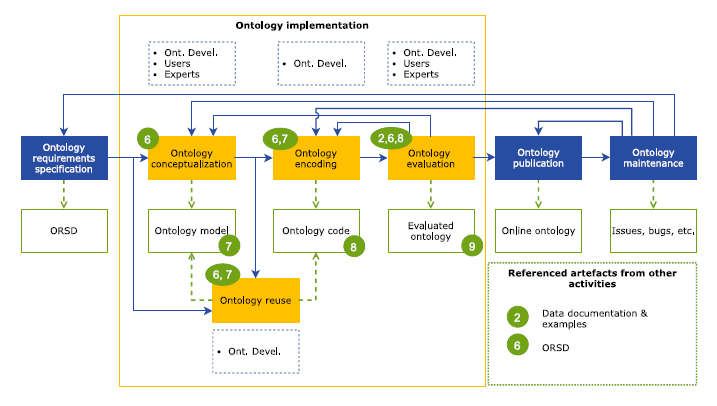
\includegraphics[width=0.9\linewidth]{Figures/fig_14.png}
    \caption{Ontology implementation workflow}
    \label{fig:enter-label}
\end{figure}
At the end of this phase, the output is an ontology read y to be published and to be made available online.

\newpage
\section{Ontology conceptualization}
The first step in the ontology implementation is the ontology conceptualization. In this phase there is the definition of all main concepts in the ontology with the relations among them. I used \href{draw.io}{https://app.diagrams.net/} software : a free easy-to-use diagramming tool that allows to represent UML diagrams and many more. I chose this software over other diagramming tools because it is intuitive, easy to use, and frequently updated moreover with draw.io it is possible to export diagrams in other formats like: svg, pdf and png in high resolution.\\
Starting from competency questions I chosed a top-down strategy in order to model the domain of prompt engineering and large language models, modeling first major concepts and then going more into detail. The idea behind the conceptualization of large language models is  taking the user's perspective: what informations are useful and meaningful to a user about large language models? From this perspective, I decided not to dwell too much on theoretical details but to focus on concepts that are useful for users in selecting the most suitable large language model for their purposes. A large language model is represented using four dimensions:
\begin{enumerate}
    \item \textbf{Type:} type of large language model which is a sub concept. Each type of large language model has one or more instances representing versions of that large language model.

    \item \textbf{Organization:} organization that creates the large language model.

    \item \textbf{Base model:} the deep learning model at the base of the architecture of the large language model. This concept represents a characteristic of a large language model.

    \item \textbf{Capability:} the capability of a large language model and it represents a characteristic of a large language model.
\end{enumerate}
These concepts provide a representation of various aspects of large language models, from their underlying architecture to the organizations that develop them, which can range from universities and research institutions to companies with business-oriented goals. A fundamental aspect is the representation of the capabilities of large language models. In fact, the ontology will not only include large language models capable of processing text but also multimodal models capable of handling more complex data types, such as images, audio, video, and source code.\\
Regarding prompt engineering, starting from the user's perspective, I decided to model the domain using the following concepts:
\begin{itemize}
    \item \textbf{Prompting technique:} this concept gathers all the prompting techniques, each prompting technique is a sub concept.

    \item \textbf{Prompt:} this is the base concept, a single prompt provided as input in the context of a chat with a specific large language model, followed by a response. The prompt can be generated using a prompting technique.

    \item \textbf{Chat:} this concept represents the context of a prompt with a specific large language model and it can include one or more prompts and responses.

    \item \textbf{Response:} this concepts reprents the response 
    generated by large language model after the input of a prompt in the context of a specific chat.
\end{itemize}
In addition there is also the modelling of the concept \textbf{"Task"} represents the tasks to be solved using large language models by applying prompting techniques. This concept has sub concepts specific for the task that has to be solved like: image task, text task, code task, audio task and video tasks, each one of those concepts has other sub concepts, for example the "text task" has as sub concepts: text summarization, emotion classification, text translation ecc. The concepts of \textbf{"Chat"} and \textbf{"Prompt"} are introduced to decouple each prompting technique from a specific large language model, ensuring their independence. The reasoning behind this conceptualization is simple and straightforward: a prompt is created using a specific prompting technique and applied in the context of a specific chat with a version of large language model producing a response. The connection with the concept of Task lies in solving a specific task through the use of an instance of a prompting technique.\\
Once defined the major concepts in the ontology, I define the relations between these concepts. Starting from the large language model, each sub concept like GPT, Mistral, Gemini is involved in the following relations:
\begin{itemize}
    \item \textit{develops:} an organization develops a large language model type, for example Google develops Gemini.

    \item \textit{has architecture:} a large language model type has architecture a specific base model, for example GPT has architecture the decoder-only model.

    \item \textit{has capability:} a large language model type has capability a specific capability and all versions have that capability. For example if GPT has capability the text processing capability, GPT-1, GPT-2, GPT-3 and GPT-4 are able to process text. In the case where a version represents an evolution of the model by introducing new capabilities, that specific version will be linked to the newly introduced capabilities, for example GPT-4 has \textit{image processing} and \textit{code processing} capabilities.
\end{itemize}
As we have seen, the aspect of different versions of the same model (GPT) must be considered and appropriately represented. To achieve this, I have used two distinct relations:
\begin{itemize}
    \item \textit{has variant:} this relation represents a contemporaneity between two models, where a model x is a variant of a model y, and this does not represent an evolution of model x. For example Mistral-7B has variant Codestral (a version of Mistral specific for source code processing.)

    \item \textit{evolves:} unlike \textit{has variant}, this relation represents a temporal succession between an older model and a newer model, for example GPT-3 evolves GPT-4, where GPT-4 is a more recent and powerful version of GPT. For this relation, I have introduced also the inverse relation \textit{evolved from}.
\end{itemize}
Another specific aspect considered is the presence of relations between organizations developing large language models, where one organization is part of another organization, for example, DeepMind is a research organization and is part of Google. I created two relations called: \textit{has organization} and \textit{is organization of} in order to represent this aspect in the ontology. In the figure below we can see the conceptualization of the part just described.
\begin{figure}[H]
    \centering
    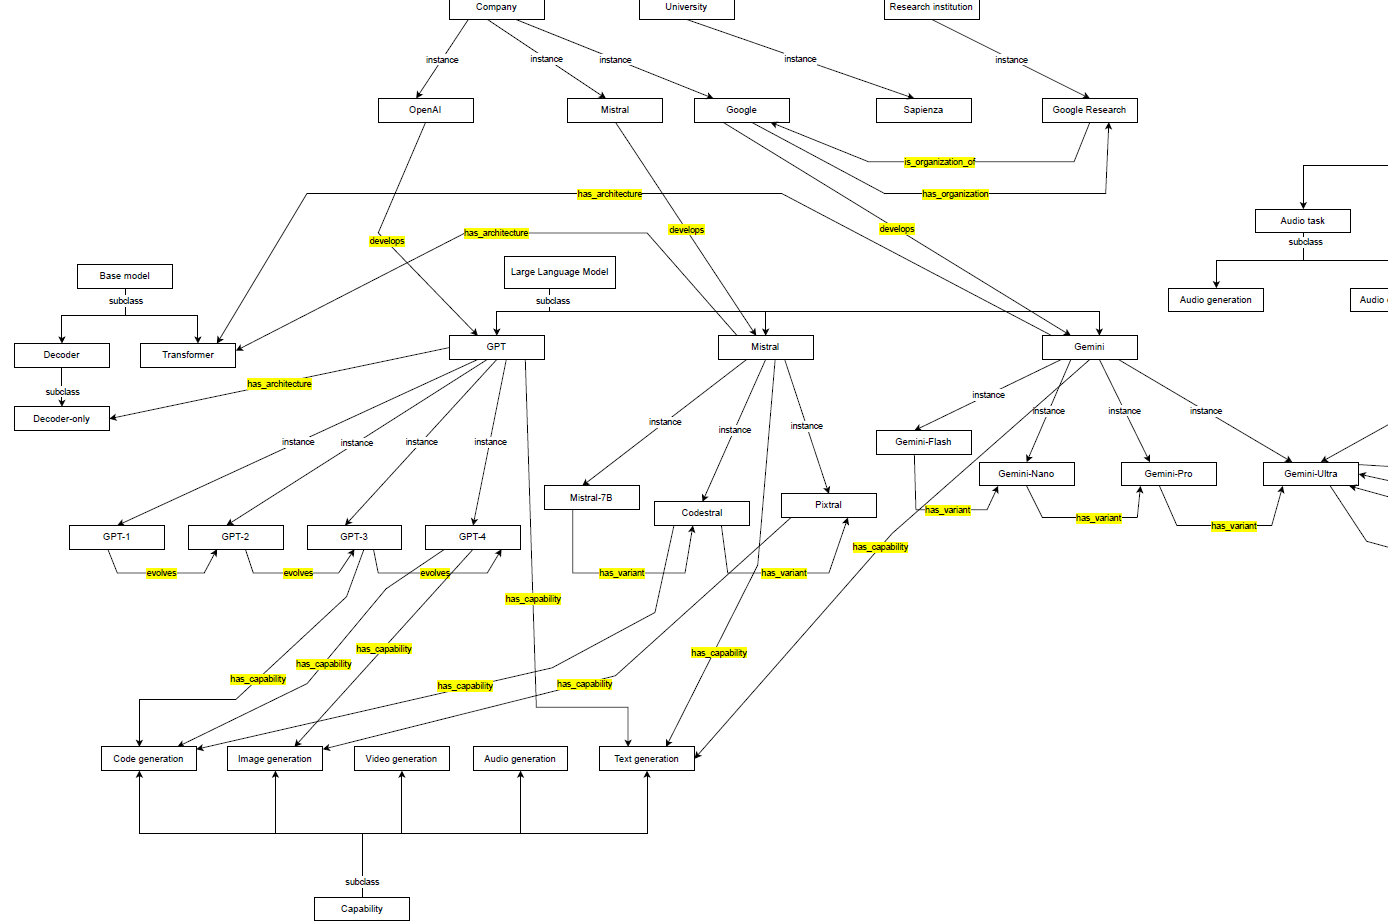
\includegraphics[width=0.9\linewidth]{Figures/fig_26.png}
    \caption{Large language models\\ dimensions conceptualization}
    \label{fig:enter-label}
\end{figure}
Regarding the prompt domain the following relations have been created in order to properly connect concepts introduced:
\begin{itemize}
    \item \textit{solves task:} this relation connects an instance of a prompting technique with an instance of a task, where the instance of the prompting technique solves that specific task. The inverse relation is: \textit{solved by}.

    \item \textit{is used in prompt:} the instance of a prompting technique is used in a specific prompt for generating the prompt using that technique. The inverse relation is: \textit{prompt generated using}.

    \item \textit{has context:} this relation connects the prompt with its context, the chat where one or more prompt are connected to. The inverse relation is: \textit{has prompt}.

    \item \textit{uses model:} this relation connects the chat with the specific model that is used to input prompts and generate responses. The inverse relation is: \textit{is used in chat}

    \item \textit{generates response:} this relation connects the specific large language model with the response generated after the input of the prompt. The inverse relation is: \textit{response generated using}.

    \item \textit{prompt follows response:} this relation connects a prompt with its response, the inverse relation is: \textit{response followed by prompt}.

    \item \textit{has response:} this relation connects the chat with the response generated by the model, the inverse relation is: \textit{is response of}. 
\end{itemize}
The conceptualization of prompt engineering domain is represented in the below diagram using draw.io

\begin{figure}[H]
    \centering
    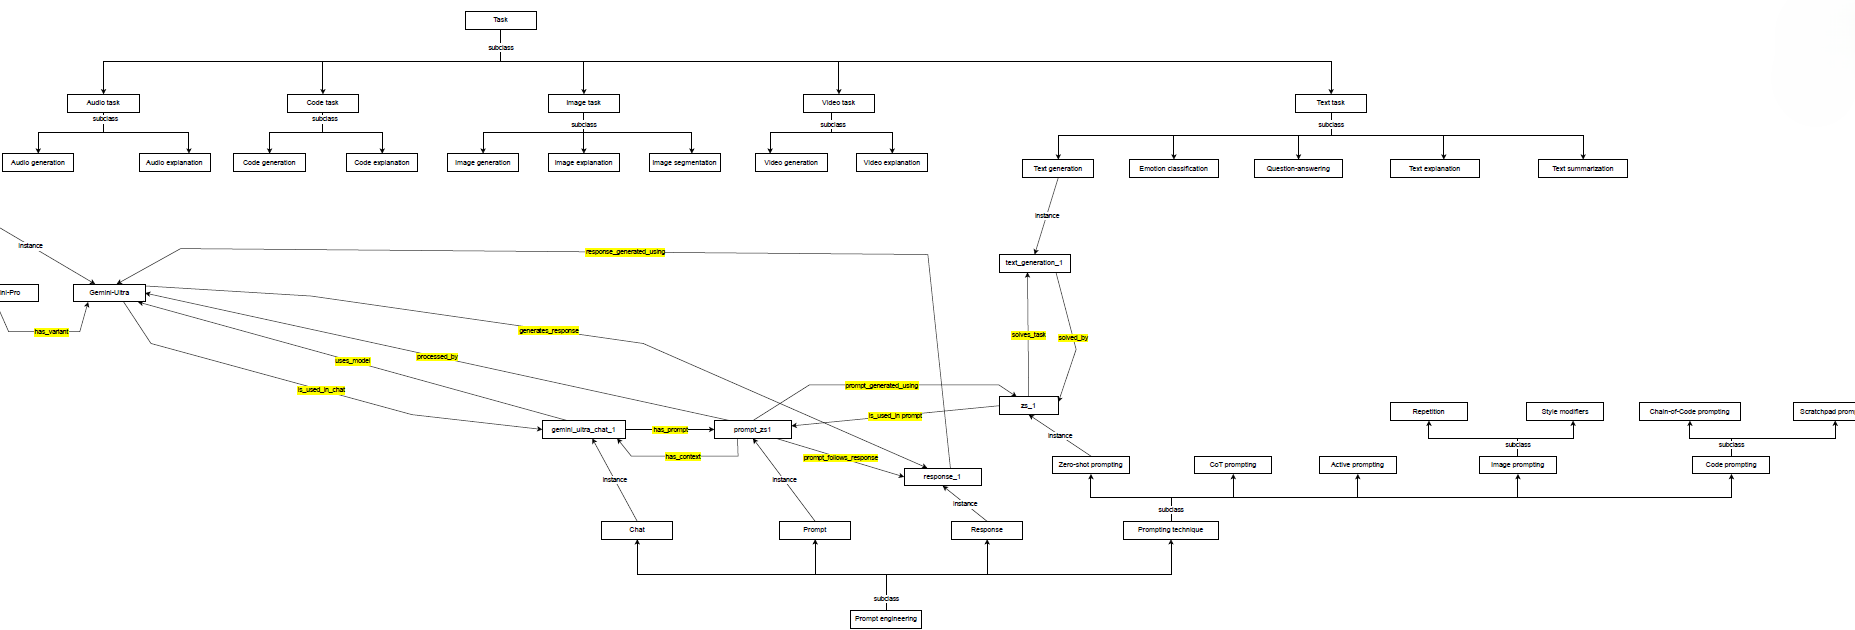
\includegraphics[width=0.9\linewidth]{Figures/fig_27.png}
    \caption{Prompt engineering\\ dimensions conceptualization}
    \label{fig:enter-label}
\end{figure}
After completing the conceptualization phase, the process can proceed to ontology reuse and ontology encoding. This involves first identifying similar ontologies within the domain of interest for potential reuse, followed by implementing and encoding the defined concepts using dedicated software tools.

\newpage
\section{Ontology reuse}
Before proceeding with ontology encoding, it is necessary to consider any similar ontologies that can be reused in the creation of the prompt engineering ontology. There are two types of reuse:
\begin{itemize}
    \item \textbf{Hard reuse:} it involves directly importing an entire ontology, rigidly incorporating it. Classes and properties are used without modification, ensuring semantic consistency but creating strong dependency on the original ontology.

    \item \textbf{Soft reuse:} it involves adapting or copying specific concepts without importing the complete ontology. This approach offers more flexibility, allowing customization, but it may introduce semantic inconsistencies or redundancies 
\end{itemize}

\subsection{Ontology design patterns reuse}


\subsection{State-of-art ontologies reuse}
I considered two ontologies that can be reused for the implementation of prompt engineering ontology:
\begin{enumerate}
    \item HALO ontology

    \item AI ontology
\end{enumerate}
The HALO ontology \cite{nananukul2024halo}, reviewed in the state-of-the-art chapter, has been considered due to its relevance to a domain closely connected to large language models, specifically addressing the hallucinations they generate. The ontology is accessible on \href{https://github.com/navapatn/halo-ontology}{Github} and despite the complete and exhaustive paper published, the published ontology is very poor. It has just twenty-five classes and non of them as an annotation or something to explain better the concept. There is a class called \textit{"LLMs Hallucination"} with two subclasses called \textit{"factuality hallucination"} and \textit{"faithfulness hallucination"} each one has subclasses about the type of hallucination that represent. Moreover there are pretty useless classes like \textit{"answers"} or \textit{"Book"} that seem have no sense in an ontology of this type, there are no individuals and just nine unused object properties. 
\begin{figure}[H]
    \centering
    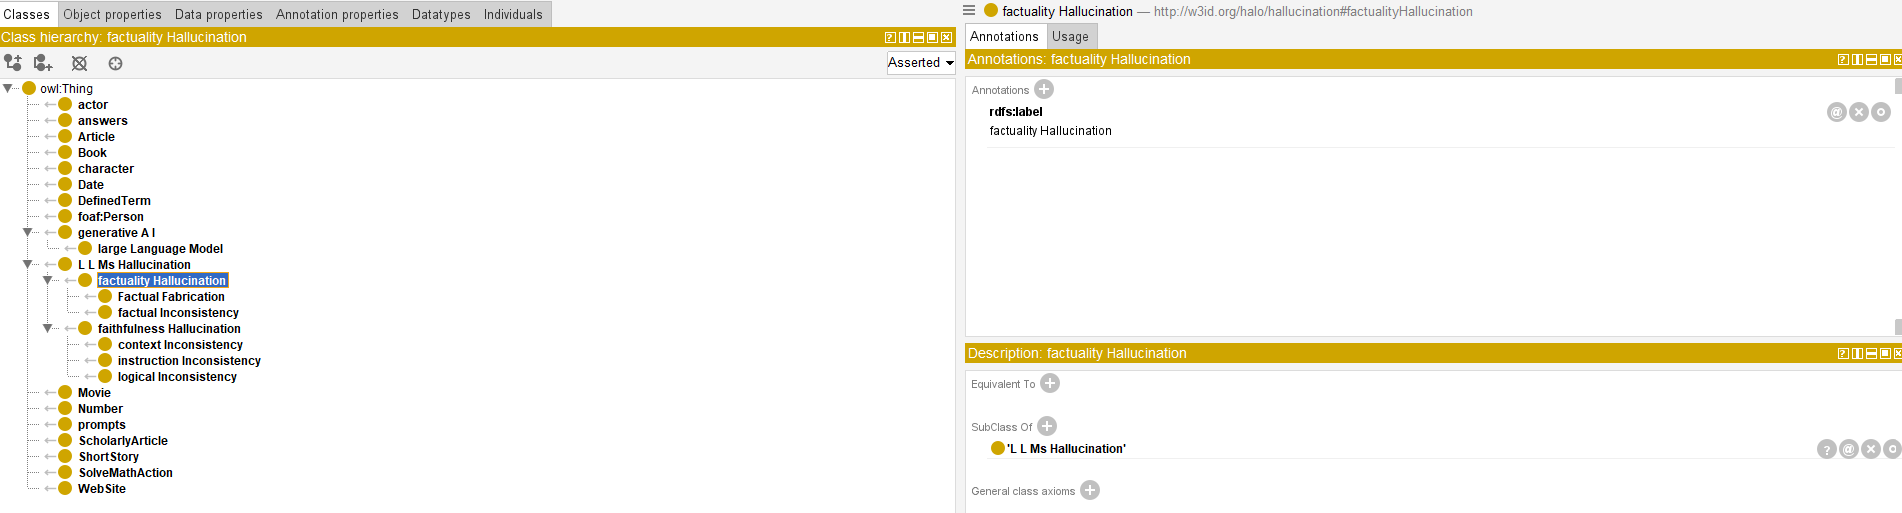
\includegraphics[width=1.0\linewidth]{Figures/fig_28.png}
    \caption{HALO ontology on Protegé}
    \label{fig:enter-label}
\end{figure}
This was sufficient to conclude that the HALO ontology would not be reused in the development of the prompt engineering ontology, as it would not offer any meaningful or valuable information.\\
The second ontology took into account is the Artificial Intelligence Ontology\cite{aio}, an ontology that covers machine learning methods, deep learning networks and their components. This ontology is particularly intriguing, as it stands out as one of the few, if not the only, ontologies focused on the field of artificial intelligence. The ontology is available on \href{https://github.com/berkeleybop/artificial-intelligence-ontology}{Github} in owl, json and csv format. Even in this case, despite the thorough study conducted, the ontology seems, in my opinion, incomplete in several aspects. Similar to the previous ontology, it includes only class labels without any additional annotations to clarify the represented concepts. The ontology is essentially a hierarchical structure, a taxonomy of concepts related to machine learning and deep learning, lacking both object properties and instances to populate the classes. The ontology, therefore, is not only useless in and of itself but, due to its lack of completeness, would not contribute any valuable information or serve as a meaningful reference for the prompt engineering ontology.\\ Prompt engineering and large language models represent a very recent field, and, as we have observed, only a few ontologies address it, often in a superficial and incomplete way. Therefore, I have chosen not to reuse any existing ontologies and to develop the prompt engineering ontology entirely from scratch. This approach allows me to represent the domain in the best possible way, without any limitations, and in a complete and clear manner.

\newpage
\section{Ontology encoding}
\subsection{Software in ontology encoding and the Protégé editor}
The ontology encoding phase is where the ontology is actually implemented. During this stage, the concepts and relationships defined in the conceptualization phase are formalized into a specific machine-readable language. Several tools are available to assist developers with this task. The main software tools for implementing ontologies include:
\begin{itemize}
    \item \href{https://protege.stanford.edu/}{Protégé}
    \item \href{https://www.cognitum.eu/semantics/fluenteditor/}{FluentEditor}
    \item \href{https://github.com/vivo-project/Vitro?tab=readme-ov-file}{Vitro}
    \item \href{https://www.semafora-systems.com/ontobroker-and-ontostudio-x}{OntoStudio}
\end{itemize}
To begin, I chose the software for my project and opted for \href{https://protege.stanford.edu/}{Protégé}: an open-source ontology editor developed by a team at Stanford University since 1987. Widely used and highly regarded among ontology engineers, it offers a user-friendly Eclipse-based interface and a wide range of features, including:
\begin{itemize}
    \item Ontology editing for OWL and RDF: it is possible to create, edit and visualize ontologies based on standard languages such as OWL (Web Ontology Language) and RDF (Resource Description Framework). 
    
    \item Reasoning and ontology validation: Protégé includes reasoning tools that allow the deduction of new information based on the rules defined in the ontology.

    \item Support for extensible plug-ins: Protégé supports a wide range of plug-ins, such as HermiT, FaCT++, and Pellet, which enhance reasoning, visualization, and ontology management capabilities.

    \item Ontology import and export: it is possible to import and export ontologies in various formats, including OWL, RDF/XML, Turtle, and JSON-LD, ensuring  compatibility with other tools and systems.

    \item Automatic documentation: Protégé supports the automatic creation of ontology documentation without any additional plug-in.

    \item SPARQL Query Support: Protégé allows users to execute SPARQL queries directly within the tool to extract specific information from the ontology.

    \item SWRL support: Protégé has the SWRL Tab which allows to define complex rules on concepts.
\end{itemize}
Only a limited number of ontology editors provide an extensive set of features tailored for developers. Moreover, several editors have remained outdated for years and suffer from lots of bugs. During the ontology development process, \href{https://git-scm.com/}{Git} was also used: a version control software to track changes made to the ontology changes that are synchronized with the \href{https://github.com/simonegramegna/peo}{GitHub repository}.
\subsection{Encoding beginning PEO ontology}
Starting from an empty page, the first thing to do is the definition of the ontology IRI (International Resource Identifier): which has to be unique and it has to refer to a standard organization. The ontology IRI of the PEO ontology is: \textit{https://w3id.org/peo\#}, this IRI will be in every entity created inside the ontology.
\begin{figure}[H]
    \centering
    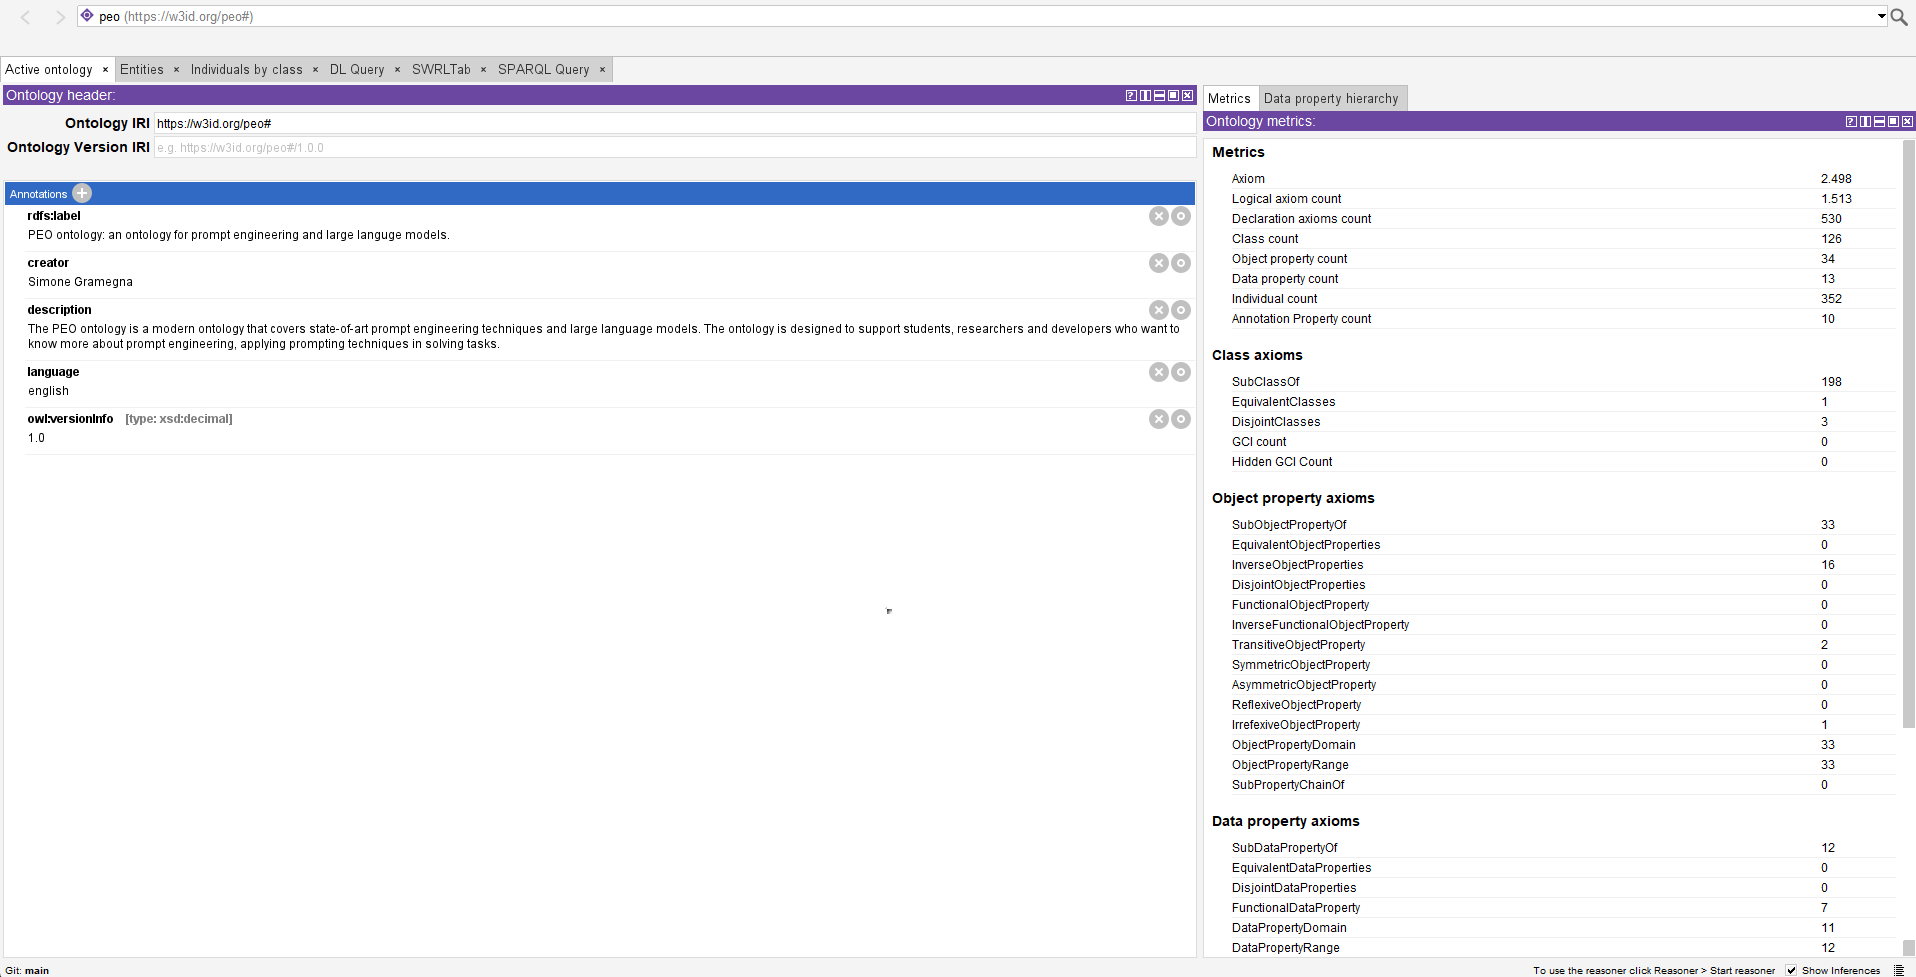
\includegraphics[width=0.8\linewidth]{Figures/fig_29.png}
    \caption{PEO ontology main page}
    \label{fig:enter-label}
\end{figure}
Once created the IRI, I defined the five annotations to properly describe the ontology:
\begin{table}[H]
    \centering
    \begin{tabular}{|>{\raggedright\arraybackslash}p{6cm}|>{\raggedright\arraybackslash}p{6cm}|}
        \hline
        \textbf{Annotation} & \textbf{Annotation value} \\ \hline
         rdfs:label & PEO ontology: an ontology for prompt 
         engineering and large language models. \\ \hline
         
         creator & Simone Gramegna\\ \hline
         
         rdfs:comment & The PEO ontology is a modern ontology that covers state-of-art prompt engineering techniques and large language models. The ontology is designed to support students, researchers and developers who want to know more about prompt engineering, applying prompting techniques in solving tasks. \\ \hline
         
         language & English \\ \hline
         
         owl:versionInfo & 1.0 \\ \hline
    \end{tabular}
    \caption{Ontology annotations in the main page}
\end{table}

Starting from the concepts outlined in the conceptualization phase, I define the primary classes of the ontology, which include:
\begin{itemize}
    \item \textbf{Base model}

    \item \textbf{Capability}

    \item \textbf{Large Language Model}

    \item \textbf{Organization}

    \item \textbf{Prompt engineering}

    \item \textbf{Task}
\end{itemize}
All these classes are mutually disjoint, as they represent distinct entities with no overlapping properties. The only exception is the relationship between "Base model" and "Capability", which are not disjoint. Both represent attributes of large language models and are collectively grouped under the \textbf{"LLM characteristic"} class, formed by the union of the two classes. \\
The Capability has five subclasses, each subclass has a label and a comment:
\begin{table}[H]
    \centering
    \begin{tabular}{|>{\raggedright\arraybackslash}p{6cm}|>{\raggedright\arraybackslash}p{6cm}|}
        \hline
        \textbf{Label} & \textbf{Comment} \\ \hline
         Audio processing &  Capability to process audio files. \\ \hline
         
         Code processing & Capability to process source code written in any programming language. \\ \hline
         
         Image processing & Capability to process images, understanding the content of the image. \\ \hline
         
         Text processing & Capability to process text and documents with text inside. \\ \hline
         
         Video processing & Capability to process video files. \\ \hline
    \end{tabular}
    \caption{Capability subclasses}
\end{table}
Each subclass has an individual with the same name, those individuals are created with the aim of assigning a capability to the instances of large language models that possess it, this aspect will be discussed later.

\subsection{Definition of large language models and characteristics}

The class "Base model" represents the models at the base of the architecture of large language models, it has six subclasses each one with label, description and reference and a subclass can have another subclass representing a more specific architecture, for example the subclass "Decoder" has inside the subclasses "Decoder only" and "Pixel decoder". 
I have included only the foundational models of the large language models represented in the ontology, excluding other base models as they fall outside the scope of this ontology. The subclasses included are: 
\begin{table}[H]
    \centering
    \begin{tabular}{|>{\raggedright\arraybackslash}p{6cm}|>{\raggedright\arraybackslash}p{6cm}|}
        \hline
        \textbf{Class} & \textbf{Subclasses} \\ \hline
         CLIP & none \\ \hline
         
         Decoder & Decoder-only, Pixel decoder \\ \hline
         
         Diffusion model & none \\ \hline
         
         Encoder & Encoder only, Global Image Encoder, Grounding Image Encoder, Region Encoder, ViT Encoder \\ \hline
         
         Recurrent Neural Network & none \\ \hline

        Transformer & Q-Former, LAMDA PT, Transformer XL \\ \hline
    \end{tabular}
    \caption{Base model subclasses}
\end{table}
The class "LLM characteristic" is subclass of both "Base model" and "Capability", each large language model subclass is connected to those two classes using the relations: \textit{has\_capability} (inverse relation \textit{is\_capability}) and\\ \textit{has\_model\_architecture}. In total there are 33 large language models subclasses of large language model, each subclass represents a type of a llm like GPT, Gemini ecc. The definition of large language models is completed with a label, a description, a link to the paper and a link to the website. Below there are large language models in the prompt engineering ontology with its own capability and architecture.
\begin{table}[H]
    \centering
    \begin{tabular}{|>{\raggedright\arraybackslash}p{4cm}|>{\raggedright\arraybackslash}p{4cm}|>{\raggedright\arraybackslash}p{4cm}|}
        \hline
        \textbf{LLM} & \textbf{Capability} & \textbf{Base model} \\ \hline
        Alpaca & Text processing & Transformer\\ \hline
        BERT & Text processing & Encoder only \\ \hline
        BLIP-2 & Image processing & Q-Former \\ \hline
        BLOOM & Text processing & Transformer \\ \hline
        Chinchilla & Text processing & Transformer \\ \hline
        Claude & Text processing & Transformer \\ \hline
        CogVLM & Image processing & ViT Encoder \\ \hline
        Command R & Text processing & Transformer \\ \hline
        DALL-E & Image processing & CLIP, Decoder, Transformer \\ \hline
        Falcon & Text processing & Decoder only \\ \hline
        FLAN & Text processing & LAMDA PT \\ \hline
        Gemini & Audio processing, Code processing, Image Processing, Text processing, Video processing & Transformer\\ \hline
        Gemma & Text processing & Transformer \\ \hline
    \end{tabular}
    \caption{Large language models in PEO ontology - part 1}
\end{table}

\begin{table}[H]
    \centering
    \begin{tabular}{|>{\raggedright\arraybackslash}p{4cm}|>{\raggedright\arraybackslash}p{4cm}|>{\raggedright\arraybackslash}p{4cm}|}
        \hline
        \textbf{LLM} & \textbf{Capability} & \textbf{Base model} \\ \hline
        GLaMM & Image processing & Global Image Encoder, Grounding Image Encoder \\ \hline
        LLaMA & Text processing & Transformer \\ \hline
        Midjourney & Image processing & Diffusion model  \\ \hline
        Minerva & Text processing & Transformer \\ \hline
        Mistral & Text processing & Transformer \\ \hline
        MPT-7B & Text processing & Decoder only \\ \hline
        OLMo & Text processing & Decoder only \\ \hline
        OpenELM & Text processing & Decoder only \\ \hline
        OPT & Text processing & Transformer \\ \hline
        PaLM & Text processing, Code processing & Transformer \\ \hline
        Phi-1 & Text processing & Transformer \\ \hline
        RWKV LLM & Text processing & Recurrent Neural Network, Transformer \\ \hline
        Sora & Video processing & Decoder only \\ \hline
        StableLM & Text processing & Decoder only \\ \hline
        StarCoder & Code processing & Decoder only \\ \hline
        T5 & Text processing & Transformer \\ \hline
        VALL-E & Audio processing & Transformer \\ \hline
        Vicuna & Text processing & Transformer \\ \hline
        XLNet & Text processing & Transformer XL \\ \hline
    \end{tabular}
    \caption{Large language models in PEO ontology - part 2}
\end{table}
There is a relation \textit{based\_on} between two subclasses of large language model (with inverse relation \textit{basis\_for}) where a large language model is developed starting from the base of another large language model. For example Alpaca is based on LLaMA (another family of large language models).\\
Each type of large language model has a capability, this capability is common for all instances of the large language model then if a specific version of a LLM has a new capability, the single LLM can be connected to that specific capability. For example GPT has capability text processing but GPT-3.5 has also the capability of code processing so this version has two capabilities (text processing and code processing). Same goes for GPT-4 which is an evolution of GPT-3.5 an it has the image processing capability, so it has three capabilities (text processing, code, processing and image processing). This approach is very flexible an efficient because there is no need to divide into categorical classes each version of large language model by simply connecting the version with the specific instance oof the capability. There are three relations between versions of the same large language model: 
\begin{itemize}
    \item \textit{has\_variant:} relation between two large language models (x and y), where x has y as another version.

    \item \textit{evolves:} transitive relation between two large language models (x and y), where y is an evolution of x. 

    \item \textit{evolved\_from:} transitive inverse relation of \textit{evolves} between two large language models x and y.
\end{itemize}
While the relation \textit{has\_variant} does not express an evolution but just a different version of the model, the relation \textit{evolves} implies also the relation \textit{has\_variant}, for example if GPT-3.5 evolves GPT-4 then GPT-3.5 has variant GPT-4, this cannot be expressed using relation but using SWRL rules. SWRL rules are are logical expressions that extend OWL ontologies by allowing the definition of conditional "if-then" rules for reasoning, those rules are processed by a reasoner during the inference. The chosed reasoner is the Hermit reasoner\cite{glimm2014hermit}: a reasoner already included in Protégé which does not require the installation of any additional plug-in. The reasoner ensures the ontology consistency, inferring new axioms and processing SWRL rules. SWRL rules are widely applied in the ontology, the first application is the creation of a new relation \textit{has\_variant} if there is the \textit{evolves} relation, the rule is expressed in this way:
\begin{lstlisting}
peo:evolves(?x, ?y) -> peo:has_variant(?x, ?y)
\end{lstlisting}
$?x$ and $?y$ express the two instances involved in the relations and the rules is applied to all instances that satisfy the condition in the body of the rule. If a model evolves into another model, the evolved model has the capabilities of the previous model, this concept is expressed using this SWRL rule:
\begin{lstlisting}
peo:evolves(?x, ?y) ^ peo:has_capability(?x, ?c) -> peo:has_capability(?y, ?c)
\end{lstlisting}
These two relations are not explicitly defined in the ontology but are inferred by the reasoner during the reasoning process, making them visible at that stage.
Each instance of large language model has two data properties associated 
\begin{itemize}
    \item \textit{has\_number\_parameters:} number of parameters of the model.

    \item \textit{has\_release\_year:} year of release of the model
\end{itemize}
Those two data properties are functional, assigning a single value of each property to the instance of the llm.\\
Large language models are developed by organizations that can be universities, research institutions and companies for business purpose, the class \textbf{Organization} contains those three subclasses (with label  and description) and each subclass has instances representing the specific organization.
\begin{table}[H]
    \centering
    \begin{tabular}{|>{\raggedright\arraybackslash}p{6cm}|>{\raggedright\arraybackslash}p{6cm}|}
        \hline
        \textbf{Subclass or organization} & \textbf{Number of entities} \\ \hline
        
        University & 2 \\ \hline
 
        Research institution & 8 \\ \hline
        
        Company & 13 \\ \hline
    \end{tabular}
    \caption{Number of organization entities}
\end{table}
Every instance of organization has two associated data properties:
\begin{itemize}
    \item \textit{registered\_name:} the official name of the organization.

    \item \textit{official\_website:} the official website of the organization.
\end{itemize}
Organization instances and large language models are connected using the \textit{develops} relation, connecting an instance of organization with an instance of large language models. We well know that an organization does not develop a single version of an LLM but the entire family (represented by the different subclasses of the large language model class) but it is not possible to have a relation between an instance and a subclass. A possible solution could be putting manually the develops relation between the company and all version developed but it would be too long. Instead of doing this process, using the \textit{has\_variant} relation previously defined, I created the following SWRL rule:
\begin{lstlisting}
peo:develops(?c, ?x) ^ peo:has_variant(?x, ?y) -> peo:develops(?c, ?y)    
\end{lstlisting}
If a company $c$ develops a large language model $?x$ and the large language model $x$ has variant another large language model (of the same type) $y$ then the company $c$ develops the llm $y$. This rule requires that the relationship \textit{has\_variant} exists among all versions of large language models or the relation \textit{evolves} should exist, in order to infer \textit{has\_variant}. For example if OpenAI develops GPT-1, GPT-1 evolves GPT-2 (has variant GPT-2) then OpenAI develops GPT-2. This process during the inference is automatic because the \textit{evolves} relation is transitive. Another SWRL rule that involves the \textit{develops} relation is the following:
\begin{lstlisting}
peo:is_organization_of(?o1, ?o2) ^ peo:develops(?o1, ?llm) -> peo:develops(?o2, ?llm)
\end{lstlisting}
If an organization $o1$ is organization of another organization $o2$ (for example DeepMind is organization of Google) and $o1$ develops a large language model then $o2$ develops the llm. This was important to specify because different researchers teams rely on other organization that finance them and provide them with resources.

\subsection{Definition of task}
The \textbf{Task} class represents task that are solved by large language models applying prompting techniques, there are five specific subclasses representing the different types of task distinguished based on the type of data to process: image, text, video, audio, or code. Each subclass has other subclasses representing the specific task for example audio generation, text translation ecc as we can see in the table below:
\begin{table}[H]
    \centering
    \begin{tabular}{|>{\raggedright\arraybackslash}p{6cm}|>{\raggedright\arraybackslash}p{6cm}|}
        \hline
        \textbf{Task type} & \textbf{Subclasses} \\ \hline
        Audio task & Audio generation, Audio explanation \\ \hline

        Video task & Video generation, Video explanation \\ \hline
    \end{tabular}
    \caption{Types of task with subclasses - part 1}
\end{table}

\begin{table}[H]
    \centering
    \begin{tabular}{|>{\raggedright\arraybackslash}p{6cm}|>{\raggedright\arraybackslash}p{6cm}|}
        \hline
        \textbf{Task type} & \textbf{Subclasses} \\ \hline
        Code task & Code generation, Code explanation \\ \hline

        Image task & Image generation, Image explanation, Image segmentation \\ \hline

        Text task & Emotion classification, Mathematical understanding, Question-Answering, Text explanation, Test generation, Text summarization, Text translation \\ \hline
    \end{tabular}
    \caption{Types of task with subclasses - part 2}
\end{table}
All of those classes have a label and a description describing shortly the task and they can have one or more instances, each instance represents a specific task of that type, it has a data property called \textit{has\_description} to specify the description of the task.

\subsection{Definition of prompt engineering}
The \textbf{Prompt engineering} class includes all concepts associated with prompts, such as their creation, the context in which they are applied, and the responses they produce. It has four main subclasses, each one with a label and a description:
\begin{itemize}
    \item \textbf{Chat:} context in which a prompt is created. 
    \item \textbf{Prompt:} input to a large language model.
    \item \textbf{Prompting technique:} technique used to create a prompt.
    \item \textbf{Response:} response given by a large language model after a prompt.
\end{itemize}
The prompting technique is very important because it has all the subclasses representing the different prompting techniques and all instances of those classes are connected using different object properties. All subclasses of Prompting Technique refer to techniques used in tasks that involve processing only textual content. Prompting techniques related to images and source code are specifically addressed by their respective subclasses \textbf{Code prompting technique} and \textbf{Image prompting techniques}, each subclass has subclasses with specific techniques. Prompting techniques for audio and video have not been specified, as the few existing techniques are experimental and not yet well-established. Moreover, for obvious reasons, they would be challenging to represent within the ontology. The prompting techniques are gathered from papers, as seen in the background chapter, each subclass representing the specific technique has a label, a description and a reference. In total there are 24 prompting techniques:
\begin{itemize}
    \item Active prompting
    \item Analogical prompting
    \item Automatic Chain-of-Thought prompting
    \item Chain-of-Knowledge prompting
    \item Chain-of-Note prompting
    \item Chain-of-Table prompting
    \item Chain-of-Thought prompting
    \item Chain-of-Verification prompting
    \item Decomposed prompting
    \item Emotion prompting
    \item Few shot prompting
    \item Graph of Thoughts prompting
    \item Least-to-most prompting
    \item Logical Chain-of-Thought prompting
    \item ReAct prompting
    \item Retrieval Augmented Generation - RAG prompting
    \item Role prompting
    \item Self consistency prompting
    \item System-2-Attention prompting
    \item Take a step back prompting
    \item Thread of Thought prompting
    \item Tree of Thoughts prompting
    \item Zero shot prompting
\end{itemize}
For code, the class Code Prompting Technique has four subclasses:
\begin{itemize}
    \item Chain-of-Code prompting
    \item Program of Thoughts prompting
    \item Scratchpad prompting
    \item Structured Chain-of-Thought prompting
\end{itemize}
Image prompting technique class has six subclasses:
\begin{itemize}
    \item Fix deformed generations prompting
    \item Lighting
    \item Quality boosters
    \item Repetition
    \item Shot type
    \item Style modifiers
\end{itemize}
To ensure the accurate and consistent representation of prompts generated using the listed techniques, instances of the Prompting Technique class are connected to instances of other Prompt Engineering subclasses via dedicated object properties, defined explicitly or inferred by the reasoner using SWRL rules. To illustrate all instances along with their associated object properties and data properties, I propose a simple task: translating the phrase \textit{"Ciao, come va?"} from Italian to English using a zero-shot prompt as input to GPT-4.\\
The first step is to create, if it does not already exist, an instance of the "Text translation" subclass of Task, which we will name \textit{"translation\_1"} assigning the data property \textit{has\_description} the string value: \textit{"Translation of the text: Ciao, come va?"}. Now I create the instance of the prompting technique that is going to solve the task, in this case we create an instance of the subclass "Zero shot prompting" called \textit{"zs\_prompting\_1"}. This instance is connected to \textit{"translation\_1"} using the object property \textit{solves\_task} with the inverse property \textit{"solved\_by"} connecting the two instances in both directions. Before creating the prompt, we create an instance of the chat class, calling it \textit{"gpt4\_chat\_1"} and connecting to the instance \textit{GPT-4} of the GPT class using the object property \textit{uses\_model} with inverse property \textit{is\_used\_in\_chat}. The chat instance has three data properties associated:
\begin{itemize}
    \item \textit{has\_chat\_title:} title of the chat, I assign it "Translation GPT-4 italian to english 1".

    \item \textit{start\_time\_chat:} start time of the chat, I assign to it the currant time while I'm writing this chapter: "29/11/2024 - 10:37"

    \item \textit{end\_time\_chat:} end time of the chat, the chat has the duration of two minutes and I assign the value: "29/11/2024 - 10:39"
\end{itemize}
Obviously those values assigned without any criteria can be modified later. Now that a context is established, the chat \textit{"gpt4\_chat\_1"}, I proceed to create the instance of the Prompt. I specify that the prompt called \textit{"zs\_1"} is created using the instance of Zero shot prompting previously defined using the object property \textit{prompt\_generated\_using} with inverse property \textit{is\_used\_in\_prompt}, in our case \textit{"zs\_1"} is generated using \textit{"zs\_prompting\_1"}. A prompt instance can have three associated data properties:
\begin{itemize}
    \item \textit{has\_instruction:} main instruction of the prompt.

    \item \textit{has\_input\_data:} data given as input to the prompt. 

    \item \textit{has\_output\_indicator:} indicator that indicates the format of the response.
\end{itemize}
For simplicity, I assign only the instruction \textit{"Translate the English text to Italian. Text: Ciao, come va? Translation:"} to the prompt, other data properties values can be added later. Now I connect the prompt with its context, the \textit{"gpt4\_chat\_1"} using the object property \textit{has\_context} with inverse relation \textit{has\_prompt} and after the creation of this relation using an SWRL rule I connect the prompt with the large language model that takes it in input. 
\begin{lstlisting}
peo:has_context(?p, ?c) ^ peo:uses_model(?c, ?m) -> peo:processed_by(?p, ?m)   
\end{lstlisting}
If a prompt $?p$ has a context the chat $?c$ and it uses the model $?m$ then $?p$ is processed by the model $?m$. This rule creates automatically during the reasoning the relation \textit{processed\_by} with inverse relation \textit{processes}. After a prompt, the llm generates a response, in PEO ontology is instance of the Response class, the value is associated using the data property \textit{has\_response\_value} and it is connected to the prompt that generated it using the object property \textit{response\_followedby\_prompt}. In order to model the "chain" prompt-responses-prompt I created the following object properties:
\begin{itemize}
    \item \textit{response\_followedby\_prompt:} the response is after a prompt.

    \item \textit{prompt\_follows\_response:} after the prompt there is a response, inverse property of \textit{response\_followedby\_prompt}.

    \item \textit{prompt\_follows\_prompt:} after the prompt there is another prompt.

    \item \textit{prompt\_followedby\_prompt:} before the prompt there is another prompt, inverse property of {prompt\_follows\_prompt}.

    \item \textit{response\_follows\_prompt:} after the response there is a prompt.

    \item \textit{prompt\_followedby\_response:} before the prompt there is a response, inverse relation of \textit{response\_follows\_prompt}. 
\end{itemize}
We can graphically see this concatenation in the following scheme:
\begin{figure}[H]
    \centering
    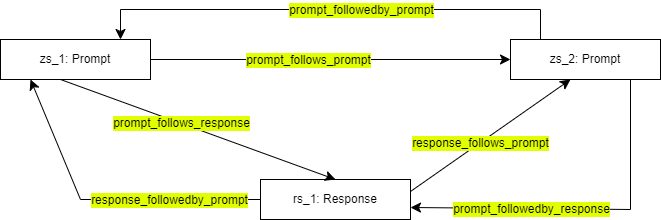
\includegraphics[width=0.9\linewidth]{Figures/fig_30.png}
    \caption{Chain prompt-response}
    \label{fig:enter-label}
\end{figure}
Of course, most of these relationships are automatically created during the inference process. To connect a response with the next prompt, I created this SWRL rule:
\begin{lstlisting}
peo:prompt_followedby_prompt(?x, ?y) ^ peo:prompt_follows_response(?y, ?r) -> peo:prompt_followedby_response(?x, ?r)
\end{lstlisting}
If a prompt $?x$ is followed by another prompt $?y$ and $?y$ has a response $?r$ then $?x$ is followed by $?r$. The context next prompt is assigned automatically using the object property \textit{prompt\_followedby\_prompt} ant this SWRL rule:
\begin{lstlisting}
peo:prompt_followedby_prompt(?x, ?y) ^ peo:has_context(?y, ?c) -> peo:has_context(?x, ?c)
\end{lstlisting}
If a prompt $x$ is followed by another prompt $y$ and $y$ has context the chat $c$ then $x$ has context $c$. Also each response is connected the chat using the object property \textit{is\_response\_of} (inverse property \textit{has\_response}) created using the SWRL rule:
\begin{lstlisting}
peo:response_followedby_prompt(?r, ?p) ^ peo:has_context(?p, ?c) -> peo:is_response_of(?r, ?c)
\end{lstlisting}
If a response $?r$ is followed by a prompt $?p$ and the prompt $?p$ has the context the chat $?c$ then the response $?r$ is response of $?c$. The last SWRL rule connects the response with the model that has generated it creating the object property \textit{response\_generated\_using} with inverse property \textit{generates\_response}:
\begin{lstlisting}
peo:response_followedby_prompt(?r, ?p) ^ peo:processed_by(?p, ?m) -> peo:response_generated_using(?r, ?m) 
\end{lstlisting}
If a response $?r$ is followed by a prompt $?p$ and the prompt $?p$ is processed by the large language model $?m$ then the response $?r$ is generated using $?m$.\\
All these object properties may seem unclear so below is a diagram that shows all the relationships involved in creating a chat.
\begin{figure}[H]
    \centering
    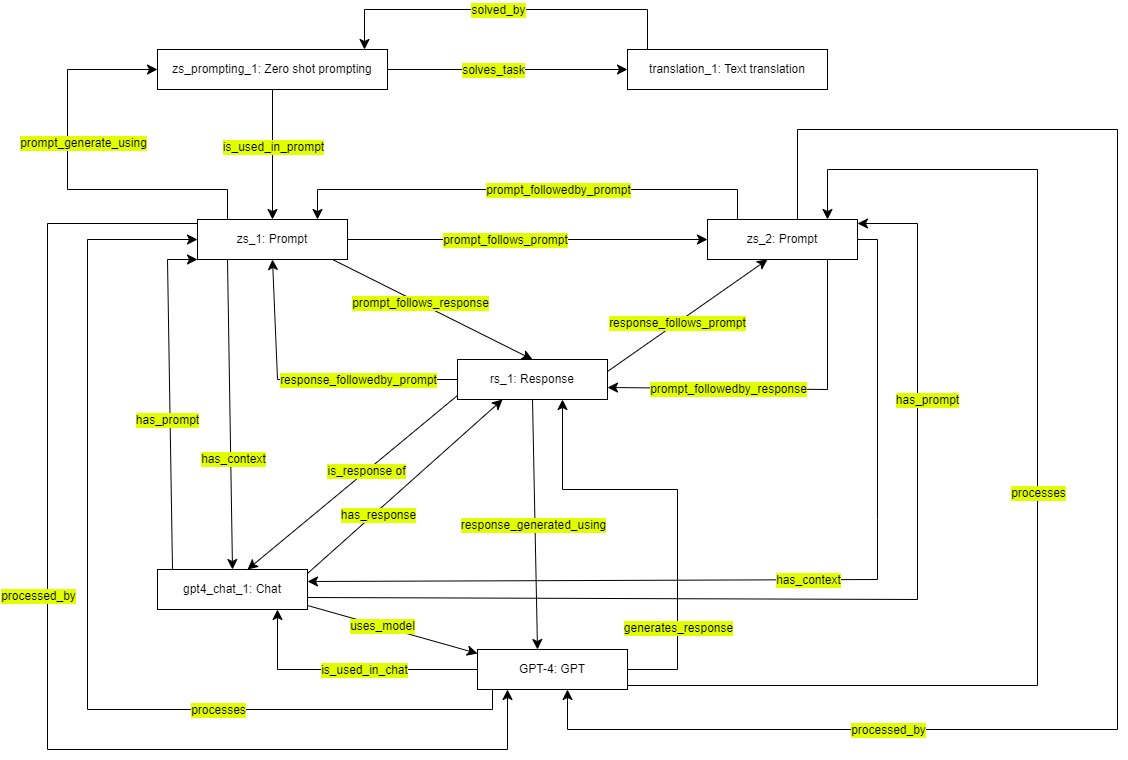
\includegraphics[width=0.85\linewidth]{Figures/fig_31.png}
    \caption{Chat scheme}
    \label{fig:enter-label}
\end{figure}


\subsection{Ontology population with prompts}
Populating the ontology with prompts is a complex process as it requires connecting various instances (task, prompting technique, prompt, chat, response, large language model) using the defined object properties. Moreover, each prompt is manually crafted in accordance with the specific prompting technique. Manually populating the ontology with all instances for every task, every version of each large language model, and every prompting technique would be highly time-consuming and beyond the objectives of this thesis. Therefore, a decision was made to populate only a specific subset of the ontology choosing large language model versions, tasks and prompting techniques. Large language models chosed are very popular LLM available to the users and they are represented in the ontology:
\begin{itemize}
    \item \textbf{GPT-4}
    \item \textbf{Mistral-7B}
    \item \textbf{Gemini Flash}
\end{itemize}
Then I chosed five prompting techniques with a criterium for each one:
\begin{itemize}
    \item \textbf{Zero-shot prompting:} this technique allows large language models to handle new tasks using only natural language instructions, without requiring examples or any effort by the user.

    \item \textbf{Few-shot prompting:} this technique  enables language models to learn new tasks with few examples, reducing the need for extensive task-specific datasets.
    
    \item \textbf{Role prompting:} this technique improves large language models performance on solving tasks by simulating specific roles.

    \item \textbf{Emotion prompting:} this technique enhances large language models by integrating emotions into prompts, improving response generation and performance on tasks.

    \item \textbf{Analogical prompting:} this technique is able to generate automatically task-specific exemplars, reducing manual annotation needs, and improving performance on problem-solving tasks.
\end{itemize}
Finally I chosed four task to solve applying prompting techniques and using large language models defined:
\begin{itemize}
    \item \textbf{Emotion classification:} classification of the emotion in a given text.

    \item \textbf{Mathematical understanding:} solving a given mathematical problem of medium difficulty. 

    \item \textbf{Text translation:} translation of a text from english to italian.

    \item \textbf{Text summarization:} summarization of the content of a given text.
\end{itemize}
Below, I list the prompts created for each task.\\\\
\textbf{Task 1: Emotion classification}\\     
The text to classify the emotion is: \textit{"I think the vacation is okay"}
\begin{itemize}
    \item \textbf{Zero-shot prompting:} Classify the text into neutral, negative or positive. Text: "I think the vacation is okay." Sentiment:
    \item \textbf{Few-shot prompting:} Classify the following text into neutral, negative, or positive based on its sentiment. Here are some examples: 
    Text: "The food was absolutely wonderful!" Sentiment: Positive. 
    Text: "I did not enjoy the movie at all." Sentiment: Negative. 
    Text: "It was an average experience." Sentiment: Neutral. 
    Now, classify this text: Text: "I think the vacation is okay." Sentiment:
    \item \textbf{Emotion prompting:} Classify the following text into neutral, negative, or positive based on its sentiment. This task is very important to my career. Please provide a well-thought and accurate classification. Text: "I think the vacation is okay." Sentiment:
    \item \textbf{Role prompting:} From now on, you are an experienced sentiment analyst with deep expertise in understanding human emotions through textual analysis. Your task is to classify the sentiment of texts as neutral, negative, or positive with utmost accuracy and professionalism. Text: "I think the vacation is okay." Sentiment:
    \item \textbf{Analogical prompting:} Classify the text into neutral, negative or positive. \# Instruction: \# Text: I think the vacation is okay. \# Sentiment:
\end{itemize}
\textbf{Task 2: Mathematical understanding}\\
For the mathematical understanding there is the solving of a simple geometrical problem: the calculation of a square with the four vertices at (-2, 2), (2, -2), (-2, -6), and (-6, -2). 
\begin{itemize}
    \item \textbf{Zero-shot prompting:} What is the area of the square with the four vertices at $(-2, 2)$, $(2, -2)$, $(-2, -6)$, and $(-6, -2)$?
    \item \textbf{Few-shot prompting:} Instruction: Determine the area of a square given the coordinates of its four vertices. 
    Example 1: Vertices: $(0, 0)$, $(4, 0)$, $(4, 4)$, $(0, 4)$ 
    Step 1: Identify the side length. Distance between $(0, 0)$ and $(4, 0)$ is $\sqrt{((4 - 0)^2 + (0 - 0)^2)} = 4$. 
    Step 2: Calculate the area. Area = side length$^2 = 4^2 = 16$. Answer: 16. 
    Example 2: Vertices: $(-1, 1)$, $(-1, 3)$, $(1, 3)$, $(1, 1)$ 
    Step 1: Identify the side length. Distance between $(-1, 1)$ and $(-1, 3)$ is $\sqrt{((3 - 1)^2 + (1 - 1)^2)} = 2$. 
    Step 2: Calculate the area. Area = side length$^2 = 2^2 = 4$. Answer: 4. 
    Query: Vertices: $(-2, 2)$, $(2, -2)$, $(-2, -6)$, $(-6, -2)$. 
    Step 1: Identify the side length by calculating the distance between consecutive vertices. 
    Step 2: Calculate the area of the square. Answer:
    \item \textbf{Emotion prompting:} Please calculate the area of a square given the coordinates of its vertices. This task is important for building my understanding of geometry and improving my analytical skills, so I truly value a thorough and accurate solution. Vertices: $(-2, 2)$, $(2, -2)$, $(-2, -6)$, $(-6, -2)$.
    \item \textbf{Role prompting:} From now on, you are a brilliant geometry teacher. You always explain geometry problems thoroughly and ensure your students understand every step of the process. I have a question for you: I have four vertices of a square: $(-2, 2)$, $(2, -2)$, $(-2, -6)$, and $(-6, -2)$. Can you help me calculate the area of the square step by step? Please provide a detailed explanation of how to verify the shape, calculate the side length, and determine the area.
    \item \textbf{Analogical prompting:} What is the area of the square with the four vertices at $(-2, 2)$, $(2, -2)$, $(-2, -6)$, and $(-6, -2)$? \# Instruction: \#\# Recall relevant exemplars: \#\# Solve the initial problem:
\end{itemize}
\textbf{Task 3: Text translation}\\
For text translation task I chosed a citation of Lewis Carol \cite{carol} to translate form english to italian: \textit{"Sometimes, I've believed as many as six impossible things before breakfast."}
\begin{itemize}
    \item \textbf{Zero-shot prompting:} Translate the English text to Italian. Text: "Sometimes, I've believed as many as six impossible things before breakfast." Translation:
    \item \textbf{Few-shot prompting:} Translate the following English sentences into Italian: 
    1. English: "Sometimes, I've believed as many as six impossible things before breakfast." Italian: "A volte, ho creduto a ben sei cose impossibili prima di colazione." 
    2. English: "I think, therefore I am." Italian: "Penso, quindi sono." 
    3. English: "All the world's a stage, and all the men and women merely players." Italian: "Tutto il mondo è un palcoscenico e tutti gli uomini e le donne sono solo attori." 
    Now translate this sentence: English: "Sometimes, I've believed as many as six impossible things before breakfast." Italian:
    \item \textbf{Emotion prompting:} Translate the following text to Italian. It's very important for me to understand this translation accurately as it could affect my professional progress: "Sometimes, I've believed as many as six impossible things before breakfast."
    \item \textbf{Role prompting:} From now on, you are an excellent literary translation teacher who accurately explains the meaning and tone of complex sentences. Translate the following sentence from English to Italian, preserving its meaning and tone: "Sometimes, I've believed as many as six impossible things before breakfast."
    \item \textbf{Analogical prompting:} \# Problem: "Sometimes, I've believed as many as six impossible things before breakfast." 
    \# Relevant Problems: 
    1. Translating a complex sentence from English to Italian. 
    - Question: How to translate the sentence "To be or not to be, that is the question" into Italian? 
    - Answer: The sentence "To be or not to be, that is the question" translates into Italian as "Essere o non essere, questo è il problema." 
    2. Translating a sentence with idiomatic expressions. 
    - Question: How to translate "Break a leg!" into Italian? 
    - Answer: The idiomatic expression "Break a leg!" translates into Italian as "In bocca al lupo!" 
    3. Translating a sentence with abstract concepts. 
    - Question: How to translate "The only limit is your imagination" into Italian? 
    - Answer: The sentence "The only limit is your imagination" translates into Italian as "L'unico limite è la tua immaginazione." 
    \# Translation of the initial problem: The sentence "Sometimes, I've believed as many as six impossible things before breakfast" translates into Italian as:
\end{itemize}
\textbf{Task 4: Text summarization}\\
The last task is the summarization of the following text about permaculture: \textit{"Permaculture is a design process mimicking the diversity, functionality and resilience of natural ecosystems. The principles and practices are drawn from traditional ecological knowledge of indigenous cultures combined with modern scientific understanding and technological innovations. Permaculture design provides a framework helping individuals and communities develop innovative, creative and effective strategies for meeting basic needs while preparing for and mitigating the projected impacts of climate change."}\cite{permaculture}
\begin{itemize}
    \item \textbf{Zero-shot prompting:} Permaculture is a design process mimicking the diversity, functionality and resilience of natural ecosystems. The principles and practices are drawn from traditional ecological knowledge of indigenous cultures combined with modern scientific understanding and technological innovations. Permaculture design provides a framework helping individuals and communities develop innovative, creative and effective strategies for meeting basic needs while preparing for and mitigating the projected impacts of climate change. Write a summary of the above text. Summary:
    \item \textbf{Few-shot prompting:} You are an expert at creating concise summaries. Below are some examples of summaries based on texts.
    Example 1: Text: The Earth orbits the Sun in an elliptical pattern, taking approximately 365.25 days to complete one orbit. This forms the basis of the Gregorian calendar year. Summary: The Earth completes an orbit around the Sun in roughly 365 days, defining the calendar year.
    Example 2: Text: Sustainable agriculture incorporates practices that maintain productivity and minimize environmental impact, such as crop rotation and organic farming. Summary: Sustainable agriculture uses eco-friendly practices like crop rotation and organic methods to maintain productivity.
    Task: Text: Permaculture is a design process mimicking the diversity, functionality, and resilience of natural ecosystems. The principles and practices are drawn from traditional ecological knowledge of indigenous cultures combined with modern scientific understanding and technological innovations. Permaculture design provides a framework helping individuals and communities develop innovative, creative, and effective strategies for meeting basic needs while preparing for and mitigating the projected impacts of climate change. Summary:
    \item \textbf{Emotion prompting:} Summarize the essence of permaculture, focusing on its innovative design process inspired by natural ecosystems. Highlight how it combines traditional ecological knowledge with modern science and technology to address climate change. This understanding is vital to my research and the future of sustainable living. Please ensure the summary is concise yet comprehensive.
    \item \textbf{Role prompting:} From now on, you are an environmental scientist who specializes in explaining complex ecological concepts in an accessible and engaging manner. Your task is to provide a concise summary of permaculture principles and their importance in addressing climate challenges.
    \item \textbf{Analogical prompting:} Problem: Summarize the definition and essence of permaculture using principles that mirror natural ecosystems and combine traditional ecological knowledge with modern science. Instruction: Recall three relevant and distinct problems or topics related to summarizing processes that focus on mimicking complex systems. Provide detailed exemplars for each recalled instance, including how the principles were extracted and utilized effectively. Use the recalled insights to structure and write the final summary.
\end{itemize}
The responses for each prompt from the three large language models have been saved in the ontology, and a chat has been created for each prompt, including a title, start time, and end time resulting in a total of 60 distinct chats.
\begin{figure}[H]
    \centering
    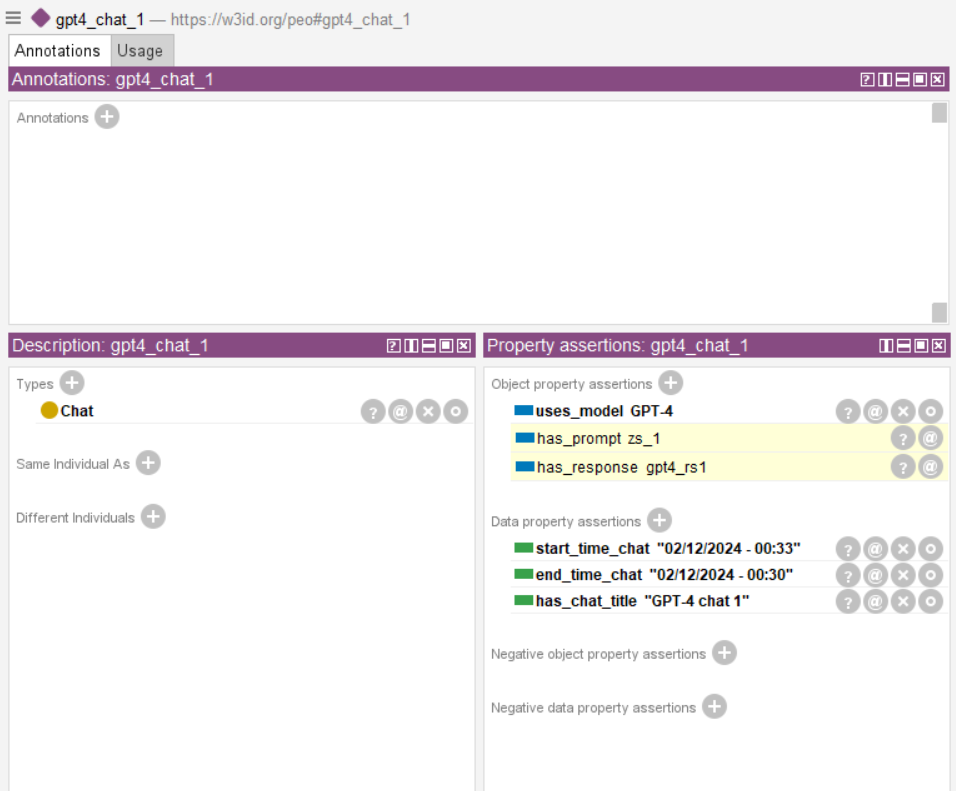
\includegraphics[width=0.75\linewidth]{Figures/fig_32.png}
    \caption{Example of chat with relations inferred}
    \label{fig:enter-label}
\end{figure}

\subsection{Automatic ontology population}
Populating an ontology with various instances can be a time-consuming task for developers, as the ontology's domain of interest often involves numerous entities requiring manual insertion. To streamline this process and reduce the developer's effort, automation can be employed. There are different researches dedicated to the automatic population of ontologies, one of the most recent is \textit{"Ontology Population using LLMs"} \cite{norouzi2024ontology}, it proposes a methodology to semi-automatically populate modular ontologies using Large Language Models (LLMs). It focuses on leveraging the strengths of LLMs, such as GPT-4 and Llama-3, for extracting structured knowledge from natural language texts. The method is divided into three main stages: data preprocessing, relevant text retrieval, and ontology population. In the first stage, the data is cleaned, organized, and aligned with simplified ontology modules to facilitate processing. The second stage employs text summarization and Retrieval-Augmented Generation (RAG) techniques to identify and extract relevant information aligned with the ontology schema. Finally, in the third stage, predefined module files guide the LLMs to populate the ontology with accurate triples by using structured prompts. Despite the good results, the methodology still requires effort, as documents need to be selected and preprocessed to create a dataset that serves as input for the large language model used to populate the ontology. Implementing this process demands skills that go beyond those of an ontology engineer, effectively shifting the workload to another task.\\ 
Another approach is proposed in the paper \textit{"Financial Product Ontology Population with Large Language Models"} \cite{saetia2024financial}, it leverages Large Language Models (LLMs), such as GPT-3.5 and GPT-4, to populate financial ontologies by extracting structured data from unstructured texts. It combines several prompting techniques to improve accuracy and scalability. Few-shot prompting provides positive and negative examples to guide the model's understanding. Chain-of-Thought (CoT) reasoning encourages sequential reasoning, while schema.org definitions are included to contextualize fields and properties. Prompts are carefully designed to generate structured outputs in JSON format for easy integration and evaluating performance using F1 scores, with the best results achieved when combining examples, CoT, and definitions. Like the previous one, this approach requires a lot of job on gathering necessary docs to pre-process and this process can be time-consuming, also the quality of the output depends on the prompts.\\ These tasks divert attention from the main objective and increase the developer's workload. Rather than using the methodologies outlined in the literature, I opted for a more straightforward and pragmatic approach to populating the ontology. Starting from the sixteen competency questions defined in the \textit{Ontology requirements specification} section, I input them, together with the ontology, into a large language model to generate an automatically populated version of the prompt engineering ontology. The large language model chosed is GPT-4o: the latest and most powerful version of GPT available in its web interface \href{https://chatgpt.com/}{ChatGPT} and used previously in the manual ontology population. This time instead of giving as input a specific prompt created with one of prompt engineering techniques, I write this prompt, providing the ontology and a text file containing the competency questions.
\begin{figure}[H]
    \centering
    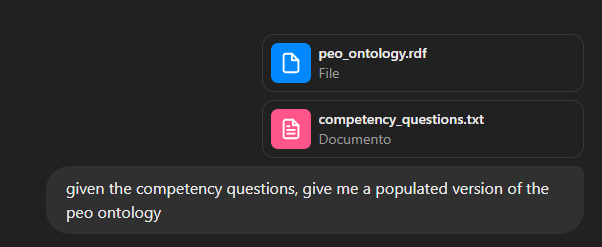
\includegraphics[width=0.9\linewidth]{Figures/fig_34.png}
    \caption{Prompt for automatic ontology population}
    \label{fig:enter-label}
\end{figure}
After this prompt the LLM begins a reasoning process, first it explains the approach followed by the model:
\begin{figure}[H]
    \centering
    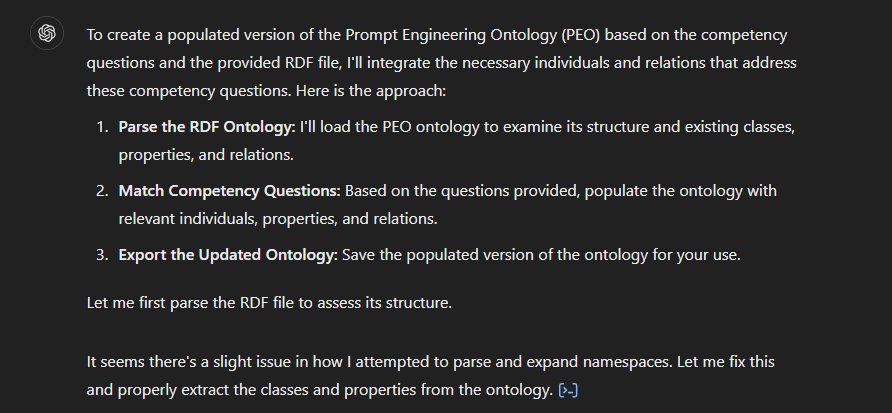
\includegraphics[width=0.9\linewidth]{Figures/fig_35.png}
    \caption{First GPT-4 output in the automatic population}
    \label{fig:enter-label}
\end{figure}
Then the model analyses the ontology structure encoded in the RDF file, listing simple classes and sample object properties found:
\begin{figure}[H]
    \centering
    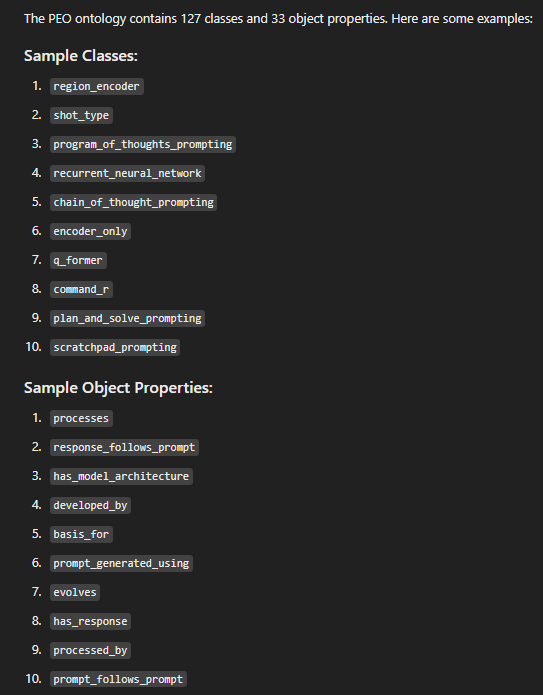
\includegraphics[width=0.85\linewidth]{Figures/fig_36.png}
    \caption{Structure analysis of the ontology}
    \label{fig:enter-label}
\end{figure}
Finally it produces the downloadable RDF file containing the ontology populated by the model:
\begin{figure}[H]
    \centering
    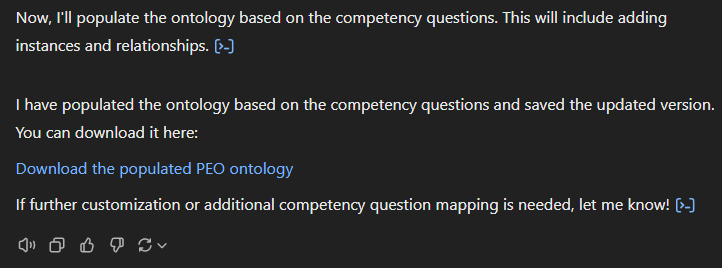
\includegraphics[width=0.9\linewidth]{Figures/fig_37.png}
    \caption{Final LLM output}
    \label{fig:enter-label}
\end{figure}
After downloading the RDF file, I open it using the Protegé editor to see the final result. At a first glance, the obtained result seems rather poor, as four new classes have been created again without considering the classes already present in the ontology:
\begin{itemize}
    \item \textbf{PromptEngineering}
    \item \textbf{Prompt}
    \item \textbf{PromptingTechnique}
    \item \textbf{Task}
\end{itemize}
without considering the hierarchy defined in the ontology as we can see:
\begin{figure}[H]
    \centering
    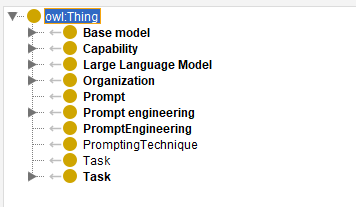
\includegraphics[width=0.9\linewidth]{Figures/fig_38.png}
    \caption{PEO ontology populated automatically}
    \label{fig:enter-label}
\end{figure}
Just two classes have a definition: Prompt and PromptEngineering with no individuals created while the PromptingTechnique class has no defintion and three individuals created:
\begin{itemize}
    \item ChainOfThoughtPrompting
    \item FewShotPrompting
    \item ZeroShotPrompting
\end{itemize}
There is no new instance of chat and all the mechanism defined to link a prompting technique with a chat is completely ignored. No new object properties or data properties have been created by GPT-4o, just an annotation property called \textit{hasDefinition}. Any other useful information is not created, the three entities are not linked with any object property and they do not have any data property. Additional prompts would clearly be needed as input for the large language model to improve the result, which is currently poor and adds no useful information compared to the original, manually populated version of the prompt engineering ontology.

\newpage
\section{Ontology evaluation}
\subsection{Ontology consistency check}
The ontology consistency check consists in running the reasoner in order to check the consistency of declared and inferenced classes and axioms, inferences are made using also SWRL rules described in the encoding section. Running the reasoner ensures also the declaration of disjointness among disjoint classes. I run the HermiT reasoner on both version of the PEO ontology: the version populated manually and the updated version made by GPT-4.\\
On the original version of the PEO ontology, the reasoner does not give any inconsistency and all the axioms are inferred correctly as we cans see below:
\begin{figure}[H]
    \centering
    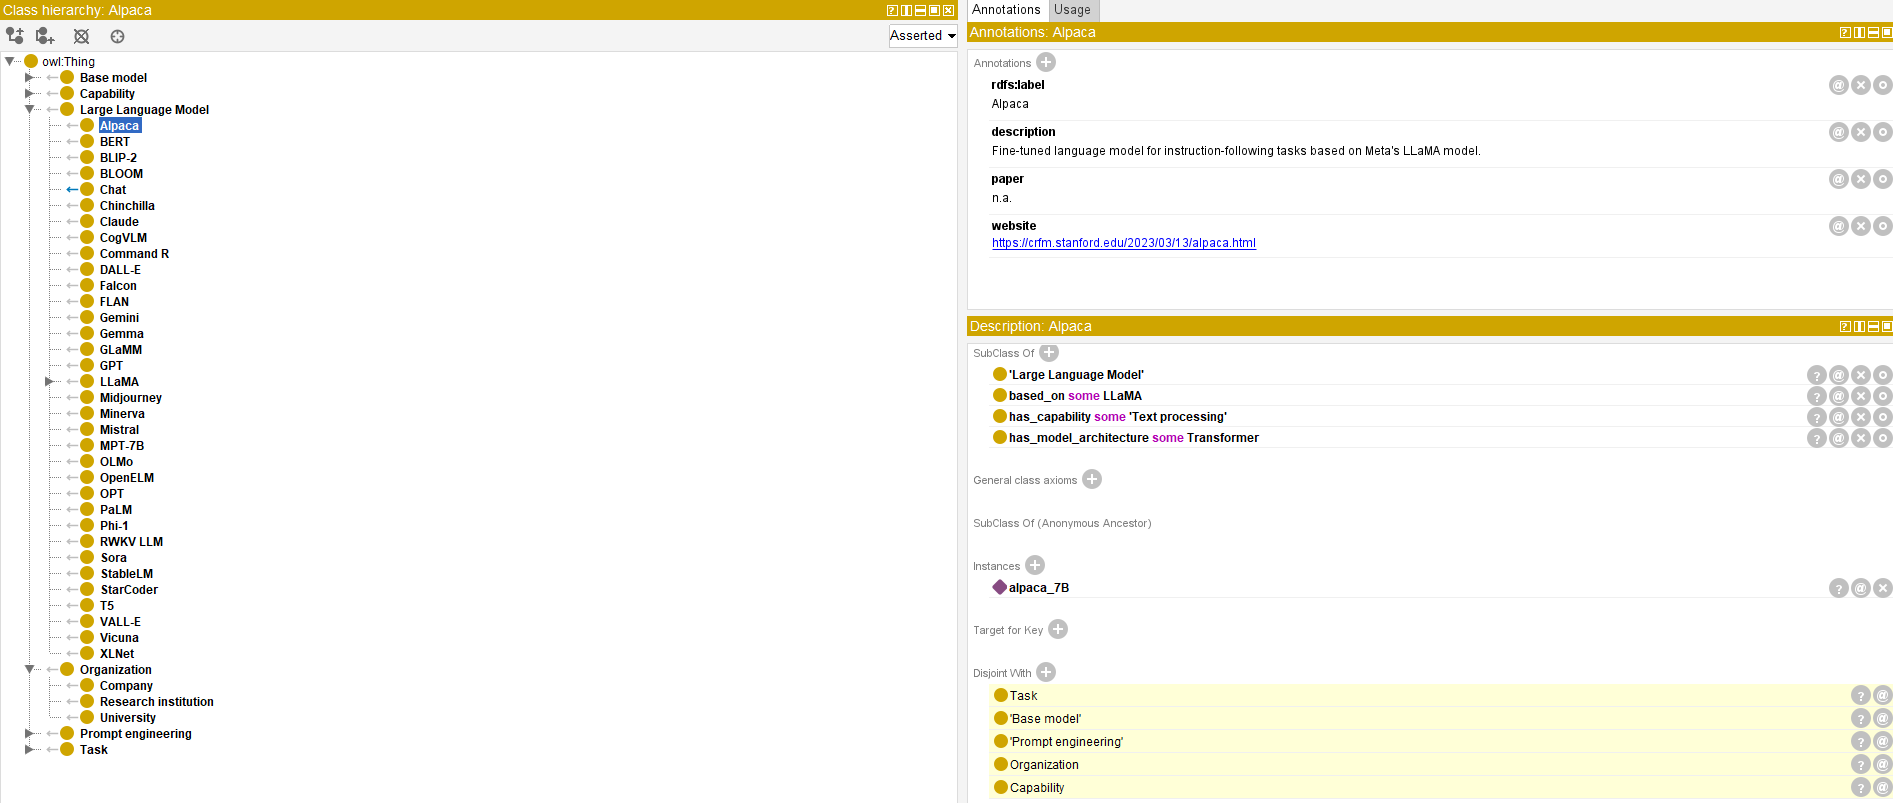
\includegraphics[width=0.9\linewidth]{Figures/fig_39.png}
    \caption{PEO ontology with HermiT reasoner}
    \label{fig:enter-label}
\end{figure}
The reasoner infers correctly that the class "Alpaca" is disjoint with the classes "Task", "Base model", "Prompt engineering", "Organization" and "Capability" because the superclass "Large language model" is declared disjoint with that list of classes. The ten SWRL rules declared work properly and inference the correct object properties for individuals:
\begin{figure}[H]
    \centering
    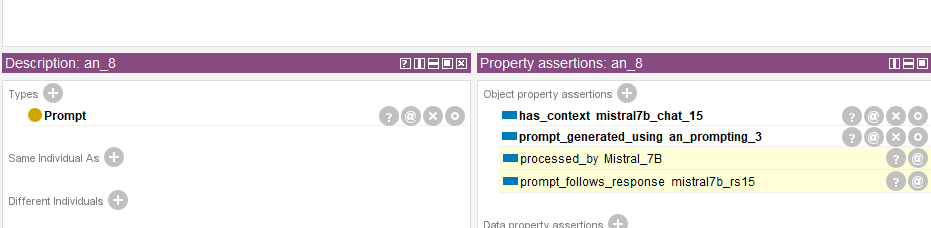
\includegraphics[width=0.9\linewidth]{Figures/fig_40.png}
    \caption{Inference on prompt individual}
    \label{fig:enter-label}
\end{figure}
The consistency check of the other version of the PEO ontology, the one populated using GPT-4 has given the exact results, this because as said in the previous section no additional significant information has been added to the ontology. The inserted classes have no link with other classes so there are no other new inferences.

\subsection{OntoMetrics}
The calculation of metrics is done using OntoMetrics: a web-based tool developed by the University of Rostock that validates and provides statistical analyses of ontologies.\cite{lantow2016ontometrics}
Given the ontology in form of RDF file or code, it calculates automatically:
\begin{itemize}
    \item Base metrics: these include simple counts of ontology elements such as classes, axioms, and objects, providing a quantitative overview of the ontology's components.

    \item Schema Metrics: these metrics evaluate the structure of the ontology's schema, considering aspects like attribute richness and inheritance richness.

    \item Knowledge base Metrics: these assess the ontology's knowledge base, focusing on the population of instances within the ontology.

    \item Class Metrics: these metrics analyse individual classes within the ontology, examining factors such as class connectivity and fullness.

    \item Graph Metrics: these evaluate the ontology's taxonomy as a graph, measuring properties like depth and breadth.
\end{itemize}
For PEO ontology, I will calculate base metrics, schema metrics and graph metrics.
\begin{figure}[H]
    \centering
    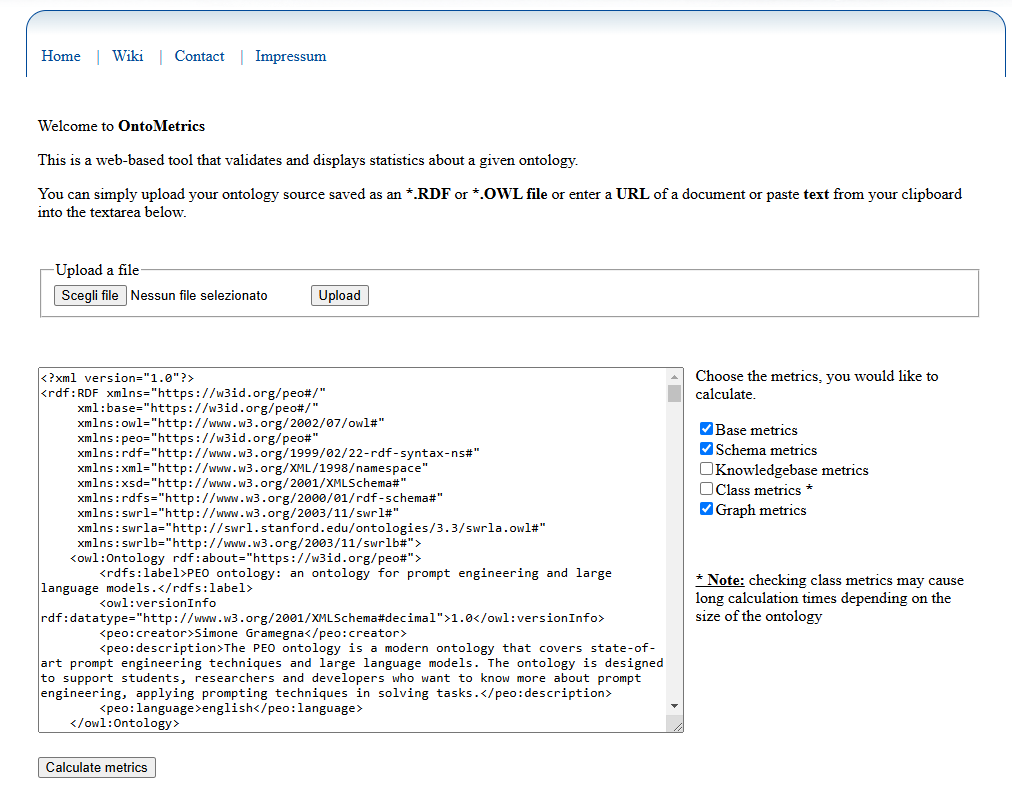
\includegraphics[width=0.9\linewidth]{Figures/fig_41.png}
    \caption{OntoMetrics interface}
    \label{fig:enter-label}
\end{figure}

Values computed for \textbf{base metrics} are:

\begin{table}[H]
    \centering
    \begin{tabular}{|>{\raggedright\arraybackslash}p{8cm}|>{\raggedright\arraybackslash}p{4cm}|}
        \hline
        \textbf{Property} & \textbf{Value} \\ \hline
        Axioms & 2684 \\ \hline
        Logical axioms count & 1695 \\ \hline
        Class count & 126 \\ \hline
        Total classes count & 126 \\ \hline
        Object property count & 34 \\ \hline
        Total object properties count & 34 \\ \hline
        Data property count & 13 \\ \hline
        Total data properties count & 13 \\ \hline
        Properties count & 47 \\ \hline
        Individual count & 352 \\ \hline
        Total individuals count & 352 \\ \hline
        DL expressivity & SRIF(D) \\ \hline
    \end{tabular}
    \caption{PEO ontology base metrics statistics}
    \label{tab:ontology-stats}
\end{table}
This table provides a high-level overview of the ontology’s structure and complexity. With 2684 axioms, the ontology is rich in detail and represents a substantial body of knowledge. Among these, 1695 logical axioms indicate a strong focus on enabling inference and reasoning. The 126 classes show that the ontology has a robust framework for organizing concepts, while 34 object properties and 13 data properties highlight the ontology’s emphasis on relationships over attribute-driven modeling. The inclusion of 352 individuals suggests that the ontology is well-populated, demonstrating practical applicability. The expressivity of SRIF(D) indicates that the ontology supports features like inverse roles and data ranges, balancing computational efficiency with expressive capability. This ontology is comprehensive but may require optimization to handle its inherent complexity effectively.

\begin{table}[H]
    \centering
    \begin{tabular}{|>{\raggedright\arraybackslash}p{8cm}|>{\raggedright\arraybackslash}p{4cm}|}
        \hline
        \textbf{Class Axiom Type} & \textbf{Count} \\ \hline
        SubClassOf axioms count & 199 \\ \hline
        Equivalent classes axioms count & 1 \\ \hline
        Disjoint classes axioms count & 3 \\ \hline
        GCICount & 0 \\ \hline
        HiddenGCICount & 0 \\ \hline
    \end{tabular}
    \caption{PEO ontology Class Axioms statistics}
    \label{tab:class-axioms}
\end{table}

This table details how classes are defined and interrelated within the ontology. The 199 SubClassOf axioms form a strong hierarchical backbone, enabling inheritance of properties and constraints. However, the limited use of equivalent classes (1) and disjoint classes (3) suggests that the ontology may not fully capture nuanced relationships or enforce strict separations between certain concepts. The absence of GCIs (Global Cardinality Restrictions) and Hidden GCIs could indicate missed opportunities to model constraints and relationships that extend across the ontology as a whole. While the current setup simplifies reasoning, incorporating more advanced axioms could enhance the ontology's semantic richness and utility.


\begin{table}[H]
    \centering
    \begin{tabular}{|>{\raggedright\arraybackslash}p{8cm}|>{\raggedright\arraybackslash}p{4cm}|}
        \hline
        \textbf{Object Property Axiom Type} & \textbf{Count} \\ \hline
        SubObjectPropertyOf axioms count & 33 \\ \hline
        Equivalent object properties axioms count & 0 \\ \hline
        Inverse object properties axioms count & 16 \\ \hline
        Disjoint object properties axioms count & 0 \\ \hline
        Functional object properties axioms count & 0 \\ \hline
        Inverse functional object properties axioms count & 0 \\ \hline
        Transitive object property axioms count & 2 \\ \hline
        Symmetric object property axioms count & 0 \\ \hline
        Asymmetric object property axioms count & 0 \\ \hline
        Reflexive object property axioms count & 0 \\ \hline
        Irreflexive object property axioms count & 1 \\ \hline
        Object property domain axioms count & 33 \\ \hline
        Object property range axioms count & 33 \\ \hline
        SubPropertyChainOf axioms count & 0 \\ \hline
    \end{tabular}
    \caption{PEO ontology Object Property Axioms Statistics}
    \label{tab:object-property-axioms}
\end{table}
Object properties are the backbone of the ontology's relational structure. With 33 SubObjectPropertyOf axioms, the ontology defines a clear hierarchy of relationships, which helps maintain organization and reasoning efficiency. The 16 inverse object properties highlight a good use of bidirectional relationships, enhancing navigability within the graph. However, the lack of functional, inverse functional, symmetric, or asymmetric properties may limit the ontology’s ability to capture specific constraints, such as unique or one-to-one relationships. The two transitive properties and one irreflexive property add some complexity but are underused. Domains and ranges are well-defined for all object properties, which is a strong point, as it ensures consistency and logical soundness in property usage.

\begin{table}[H]
    \centering
    \begin{tabular}{|>{\raggedright\arraybackslash}p{8cm}|>{\raggedright\arraybackslash}p{4cm}|}
        \hline
        \textbf{Data Property Axiom Type} & \textbf{Count} \\ \hline
        SubDataPropertyOf axioms count & 12 \\ \hline
        Equivalent data properties axioms count & 0 \\ \hline
        Disjoint data properties axioms count & 0 \\ \hline
        Functional data property axioms count & 7 \\ \hline
        Data property domain axioms count & 11 \\ \hline
        Data property range axioms count & 12 \\ \hline
    \end{tabular}
    \caption{PEO ontology Data Property Axioms Statistics}
    \label{tab:data-property-axioms}
\end{table}

Data properties focus on attributes of individuals. The 12 SubDataPropertyOf axioms indicate some level of organization, but the absence of equivalent or disjoint data properties suggests limited semantic relationships among these properties. Seven functional data properties point to a partial emphasis on ensuring that certain attributes have unique values (e.g., “hasID”), but this aspect could be expanded. Domains and ranges are defined for most properties, which improves clarity and reasoning, but the relatively low overall count of data property axioms might limit the ontology's ability to model detailed attributes of classes or individuals.

\begin{table}[H]
    \centering
    \begin{tabular}{|>{\raggedright\arraybackslash}p{8cm}|>{\raggedright\arraybackslash}p{4cm}|}
        \hline
        \textbf{Individual Axiom Type} & \textbf{Count} \\ \hline
        Class assertion axioms count & 352 \\ \hline
        Object property assertion axioms count & 390 \\ \hline
        Data property assertion axioms count & 580 \\ \hline
        Negative object property assertion axioms count & 0 \\ \hline
        Negative data property assertion axioms count & 0 \\ \hline
        Same individuals axioms count & 0 \\ \hline
        Different individuals axioms count & 0 \\ \hline
    \end{tabular}
    \caption{PEO ontology Individual Axioms Statistics}
    \label{tab:individual-axioms}
\end{table}

This table reflects how individuals are represented and connected within the ontology. The 352 class assertions and 390 object property assertions indicate that the ontology’s individuals are well-categorized and interlinked. The 580 data property assertions further show that these individuals have descriptive attributes. However, the absence of negative assertions (both object and data properties) and no axioms for declaring individuals as equivalent or distinct may limit the ontology's ability to handle complex scenarios, such as resolving conflicts or managing redundancy.

\begin{table}[H]
    \centering
    \begin{tabular}{|>{\raggedright\arraybackslash}p{8cm}|>{\raggedright\arraybackslash}p{4cm}|}
        \hline
        \textbf{Annotation Axiom Type} & \textbf{Count} \\ \hline
        Annotation axioms count & 5 \\ \hline
        Annotation assertion axioms count & 459 \\ \hline
        Annotation property domain axioms count & 0 \\ \hline
        Annotation property range axioms count & 0 \\ \hline
    \end{tabular}
    \caption{PEO ontology Annotation Axioms Statistics}
    \label{tab:annotation-axioms}
\end{table}
Annotations are crucial for documentation and understanding. With 459 annotation assertions, the ontology appears well-documented, providing metadata that can improve usability and comprehension. However, the absence of domain and range axioms for annotation properties suggests that these annotations are not constrained formally, which could lead to inconsistencies or reduced clarity in large-scale applications. Better structuring of annotation properties could enhance the ontology’s maintainability.\\
The \textbf{Schema metrics} computed for PEO ontology are: 

\begin{table}[H]
    \centering
    \begin{tabular}{|>{\raggedright\arraybackslash}p{8cm}|>{\raggedright\arraybackslash}p{4cm}|}
        \hline
        \textbf{Metric} & \textbf{Value} \\ \hline
        Attribute richness & 0.103175 \\ \hline
        Inheritance richness & 1.579365 \\ \hline
        Relationship richness & 0.160338 \\ \hline
        Attribute class ratio & 0.0 \\ \hline
        Equivalence ratio & 0.007937 \\ \hline
        Axiom/class ratio & 21.301587 \\ \hline
        Inverse relations ratio & 0.390244 \\ \hline
        Class/relation ratio & 0.531646 \\ \hline
    \end{tabular}
    \caption{PEO ontology Schema Metrics}
    \label{tab:ontology-metrics}
\end{table}
This table evaluates the structural aspects of the ontology. The attribute richness (0.103175) indicates that relatively few classes have associated attributes, which could limit the detail available for each class. The inheritance richness (1.579365) shows that most classes are part of meaningful hierarchies, a positive sign of structure. However, the relationship richness (0.160338) is relatively low, suggesting that the ontology focuses more on defining concepts than on interconnecting them. The axiom-to-class ratio (21.301587) highlights a dense ontology, meaning each class has substantial associated information, which can be both a strength and a source of complexity. Finally, the inverse relations ratio (0.390244) indicates a good but incomplete use of inverse properties to enhance navigability.\\
The \textbf{Graph metrics} for PEO ontology are:
\begin{table}[H]
    \centering
    \begin{tabular}{|>{\raggedright\arraybackslash}p{8cm}|>{\raggedright\arraybackslash}p{4cm}|}
        \hline
        \textbf{Metric} & \textbf{Value} \\ \hline
        Absolute root cardinality & 7 \\ \hline
        Absolute leaf cardinality & 109 \\ \hline
        Absolute sibling cardinality & 126 \\ \hline
        Absolute depth & 318 \\ \hline
        Average depth & 2.52381 \\ \hline
        Maximal depth & 4 \\ \hline
        Absolute breadth & 126 \\ \hline
        Average breadth & 7.0 \\ \hline
        Maximal breadth & 33 \\ \hline
        Ratio of leaf fan-outness & 0.865079 \\ \hline
        Ratio of sibling fan-outness & 1.0 \\ \hline
        Tangledness & 0.269841 \\ \hline
        Total number of paths & 126 \\ \hline
        Average number of paths & 31.5 \\ \hline
    \end{tabular}
    \caption{PEO ontology Graph Metrics}
    \label{tab:cardinality-depth-metrics}
\end{table}
Graph metrics provide insights into the topology of the ontology. The absolute root cardinality (7) and absolute leaf cardinality (109) indicate a moderately deep hierarchy with good granularity at the leaf level. The maximal depth (4) and average depth (2.52381) suggest a shallow graph, which can make the ontology easier to understand but may oversimplify complex domains. The tangledness (0.269841) is moderate, indicating a graph structure that is connected but not overly complex. The high sibling fan-out ratio (1.0) shows that sibling classes are evenly distributed, while the ratio of leaf fan-outness (0.865079) implies a balanced spread of subclasses from intermediate nodes.\\
Despite there being no significant differences between the original version of the PEO ontology and the version populated using GPT-4, I proceed to calculate metrics.\\
Values computed for base metrics are:
\begin{table}[H]
    \centering
    \begin{tabular}{|>{\raggedright\arraybackslash}p{8cm}|>{\raggedright\arraybackslash}p{4cm}|}
        \hline
        \textbf{Property} & \textbf{Value} \\ \hline
        Axioms & 2705 \\ \hline
        Logical axioms count & 1710 \\ \hline
        Class count & 128 \\ \hline
        Total classes count & 128 \\ \hline
        Object property count & 34 \\ \hline
        Total object properties count & 34 \\ \hline
        Data property count & 13 \\ \hline
        Total data properties count & 13 \\ \hline
        Properties count & 47 \\ \hline
        Individual count & 359 \\ \hline
        Total individuals count & 359 \\ \hline
        DL expressivity & SRIF(D) \\ \hline
    \end{tabular}
    \caption{PEO ontology updated base metrics statistics}
    \label{tab:ontology-stats-updated}
\end{table}

\begin{table}[H]
    \centering
    \begin{tabular}{|>{\raggedright\arraybackslash}p{8cm}|>{\raggedright\arraybackslash}p{4cm}|}
        \hline
        \textbf{Class Axiom Type} & \textbf{Count} \\ \hline
        SubClassOf axioms count & 197 \\ \hline
        Equivalent classes axioms count & 1 \\ \hline
        Disjoint classes axioms count & 3 \\ \hline
        GCICount & 0 \\ \hline
        HiddenGCICount & 0 \\ \hline
    \end{tabular}
    \caption{PEO ontology updated Class Axioms Statistics}
    \label{tab:class-axioms-updated}
\end{table}

\begin{table}[H]
    \centering
    \begin{tabular}{|>{\raggedright\arraybackslash}p{8cm}|>{\raggedright\arraybackslash}p{4cm}|}
        \hline
        \textbf{Object Property Axiom Type} & \textbf{Count} \\ \hline
        SubObjectPropertyOf axioms count & 33 \\ \hline
        Equivalent object properties axioms count & 0 \\ \hline
        Inverse object properties axioms count & 16 \\ \hline
        Disjoint object properties axioms count & 0 \\ \hline
        Functional object properties axioms count & 0 \\ \hline
        Inverse functional object properties axioms count & 0 \\ \hline
        Transitive object property axioms count & 8 \\ \hline
        Symmetric object property axioms count & 1 \\ \hline
        Asymmetric object property axioms count & 0 \\ \hline
        Reflexive object property axioms count & 0 \\ \hline
        Irreflexive object property axioms count & 1 \\ \hline
        Object property domain axioms count & 33 \\ \hline
        Object property range axioms count & 33 \\ \hline
        SubPropertyChainOf axioms count & 0 \\ \hline
    \end{tabular}
    \caption{PEO ontology updated Object Property Axioms Statistics}
    \label{tab:object-property-axioms-updated}
\end{table}

\begin{table}[H]
    \centering
    \begin{tabular}{|>{\raggedright\arraybackslash}p{8cm}|>{\raggedright\arraybackslash}p{4cm}|}
        \hline
        \textbf{Data Property Axiom Type} & \textbf{Count} \\ \hline
        SubDataPropertyOf axioms count & 12 \\ \hline
        Equivalent data properties axioms count & 0 \\ \hline
        Disjoint data properties axioms count & 0 \\ \hline
        Functional data property axioms count & 7 \\ \hline
        Data property domain axioms count & 12 \\ \hline
        Data property range axioms count & 12 \\ \hline
    \end{tabular}
    \caption{PEO ontology updated Data Property Axioms Statistics}
    \label{tab:data-property-axioms-updated}
\end{table}

\begin{table}[H]
    \centering
    \begin{tabular}{|>{\raggedright\arraybackslash}p{8cm}|>{\raggedright\arraybackslash}p{4cm}|}
        \hline
        \textbf{Individual Axiom Type} & \textbf{Count} \\ \hline
        Class assertion axioms count & 358 \\ \hline
        Object property assertion axioms count & 393 \\ \hline
        Data property assertion axioms count & 580 \\ \hline
        Negative object property assertion axioms count & 0 \\ \hline
        Negative data property assertion axioms count & 0 \\ \hline
        Same individuals axioms count & 0 \\ \hline
        Different individuals axioms count & 0 \\ \hline
    \end{tabular}
    \caption{PEO ontology updated Individual Axioms Statistics}
    \label{tab:individual-axioms-updated}
\end{table}

\begin{table}[H]
    \centering
    \begin{tabular}{|>{\raggedright\arraybackslash}p{8cm}|>{\raggedright\arraybackslash}p{4cm}|}
        \hline
        \textbf{Annotation Axiom Type} & \textbf{Count} \\ \hline
        Annotation axioms count & 5 \\ \hline
        Annotation assertion axioms count & 456 \\ \hline
        Annotation property domain axioms count & 0 \\ \hline
        Annotation property range axioms count & 0 \\ \hline
    \end{tabular}
    \caption{PEO ontology updated Annotation Axioms Statistics}
    \label{tab:annotation-axioms-updated}
\end{table}

The schema metrics for the update version of PEO ontology are:
\begin{table}[H]
    \centering
    \begin{tabular}{|>{\raggedright\arraybackslash}p{8cm}|>{\raggedright\arraybackslash}p{4cm}|}
        \hline
        \textbf{Metric} & \textbf{Value} \\ \hline
        Attribute richness & 0.101563 \\ \hline
        Inheritance richness & 1.539063 \\ \hline
        Relationship richness & 0.161702 \\ \hline
        Attribute class ratio & 0.0 \\ \hline
        Equivalence ratio & 0.007813 \\ \hline
        Axiom/class ratio & 21.132813 \\ \hline
        Inverse relations ratio & 0.390244 \\ \hline
        Class/relation ratio & 0.544681 \\ \hline
    \end{tabular}
    \caption{PEO ontology Schema Metrics}
    \label{tab:ontology-metrics-updated}
\end{table}

The graph metrics for updated version of PEO ontology are:

\begin{table}[H]
    \centering
    \begin{tabular}{|>{\raggedright\arraybackslash}p{8cm}|>{\raggedright\arraybackslash}p{4cm}|}
        \hline
        \textbf{Metric} & \textbf{Value} \\ \hline
        Absolute root cardinality & 11 \\ \hline
        Absolute leaf cardinality & 111 \\ \hline
        Absolute sibling cardinality & 128 \\ \hline
        Absolute depth & 316 \\ \hline
        Average depth & 2.46875 \\ \hline
        Maximal depth & 4 \\ \hline
        Absolute breadth & 128 \\ \hline
        Average breadth & 7.111111 \\ \hline
        Maximal breadth & 33 \\ \hline
        Ratio of leaf fan-outness & 0.867188 \\ \hline
        Ratio of sibling fan-outness & 1.0 \\ \hline
        Tangledness & 0.265625 \\ \hline
        Total number of paths & 128 \\ \hline
        Average number of paths & 32.0 \\ \hline
    \end{tabular}
    \caption{PEO ontology updated Graph Metrics}
    \label{tab:cardinality-depth-metrics-updated}
\end{table}
The new values calculated by OntoMetrics on the updated version of the ontology do not differ significantly from the previously calculated values, as the large language model GPT-4 has only added four new classes and three new instances. All results for PEO ontology and its second version are on \href{https://github.com/simonegramegna/peo/tree/main/evaluation}{Github}.

\newpage
\subsection{OOPS! validation}
The methods discussed so far are widely used in ontology evaluation; however, they are not capable of capturing modelling errors in greater detail. These errors can compromise not only the quality and usability of the ontology but also lead to potential inconsistencies. Therefore, it is necessary to adopt a different approach from those previously examined, OntoMetrics and the HermiT reasoner because they have the following issues:
\begin{itemize}
    \item OntoMetrics: it provides a quantitative measure of ontology's structural characteristics without analysing qualitative aspects, so it is not able to detect semantic and usability issues in the ontology.

    \item HermiT reasoner (reasoners in general): reasoners are designed to check the logical consistency of an ontology and perform inferencing identifying inconsistencies in axioms. But reasoners are not able to detect errors outside logical inconsistencies, such as missing domain or range definitions and they cannot check best-practice violation and usability issues.
\end{itemize}
These limitations highlight the need for a tool that can go beyond structural and logical evaluation, addressing both semantic and usability dimensions of ontology quality. \textbf{OOPS!} (Ontology Pitfall Scanner) is an online tool for ontology evaluation \cite{poveda2014oops} that automates the evaluation process without requiring any effort by the developer. 
\begin{figure}[H]
    \centering
    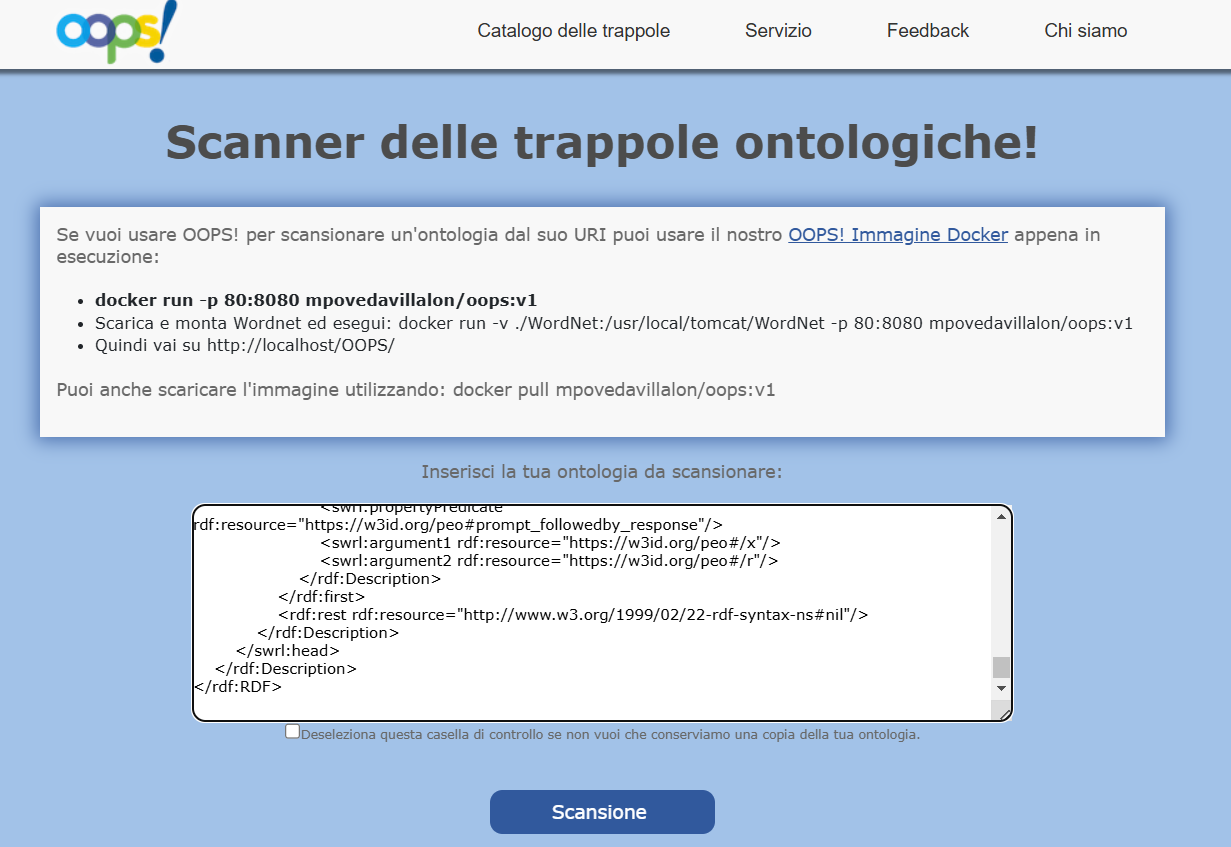
\includegraphics[width=0.9\linewidth]{Figures/fig_42.png}
    \caption{OOPS! web interface}
    \label{fig:enter-label}
\end{figure}
Given the input ontology, OOPS is able to detect 40 different pitfall that are classified into three categories: critical, important and minor by parsing the RDF code and generating a complete response using the OOPS! scanner. Pitfalls in the scanner include:
\begin{itemize}
    \item Structural pitfalls: these involve issues related to the ontology's formal structure and syntax like cycles in hierarchy and unconnected ontology elements.

    \item Functional pitfalls: these involve issues to the intended use and functionality of the ontology like missing domain or incorrectly defined inverse relationships.

    \item Usability and Profiling Pitfalls: these involve issues  affecting the ontology's clarity, maintainability, and human-readability like missing annotations, inconsistent naming and ambiguous terms.
\end{itemize}
I will use OOPS! scanner on both versions of the PEO ontology detecting and explaining found pitfalls. 
For the first version of PEO ontology there are just three pitfalls:
\begin{figure}[H]
    \centering
    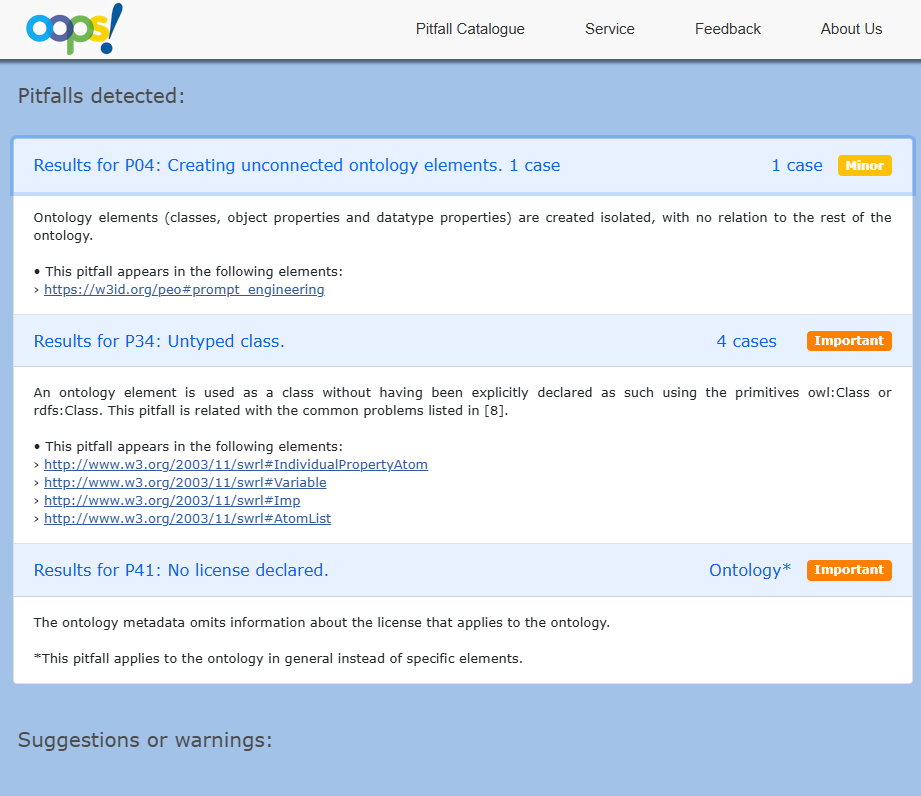
\includegraphics[width=0.9\linewidth]{Figures/fig_43.png}
    \caption{Detected pitfalls PEO ontology}
    \label{fig:enter-label}
\end{figure}
The explanation of detected pitfall is:
\begin{itemize}
    \item \textbf{P04 (Creating unconnected ontology elements):} this pitfall involves ontology elements (classes, object properties and datatype properties) are created isolated, with no relation to the rest of the ontology. In the case of PEO ontology, the \textit{prompt\_engineering} class has no relation: this because the prompt engineering class is intended as a theoretical concept with no relations with other classes.

    \item \textbf{P34 (Untyped class):} this pitfalls involves all ontology elements that are used as a class without having explicitly declared. This pitfall involves four elements in PEO ontology: \\ \textit{http://www.w3.org/2003/11/swrl\#IndividualPropertyAtom},\\ \textit{http://www.w3.org/2003/11/swrl\#Variable},\\ \textit{http://www.w3.org/2003/11/swrl\#Imp} and \\\textit{http://www.w3.org/2003/11/swrl\#AtomList}.
    This pitfall depends in the declaration of SWRL rules using the Protegé editor and it does not depend on the developer.

    \item \textbf{P41 (No license declared):} there is no license in the ontology metadata. The license of PEO ontology is specified in the Github repository.
    
\end{itemize}
Overall, the report is satisfactory, as no critical pitfalls have been identified, nor any issues found in the main classes or object properties of the ontology. The complete report is available \href{https://github.com/simonegramegna/peo/blob/main/evaluation/oops_report_peo.xml}{here}. After detecting pitfalls in the original version of the PEO ontology, I also examined the populated version generated using GPT-4 nonetheless, no significant differences were observed between the two versions. Compared to the three pitfalls identified in the previous version, OOPS detects five pitfalls:
\begin{figure}[H]
    \centering
    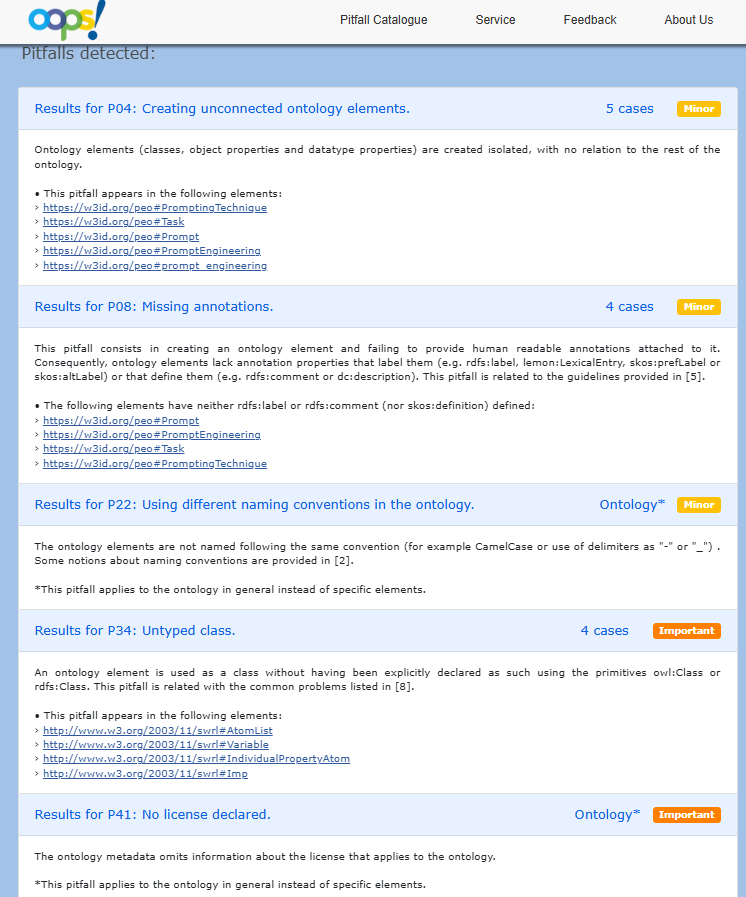
\includegraphics[width=0.75\linewidth]{Figures/fig_44.png}
    \caption{Detected pitfalls second version PEO ontology}
    \label{fig:enter-label}
\end{figure}


\begin{itemize}
    \item \textbf{P04 (Creating unconnected ontology elements):} this pitfall, as said before, involves unconnected ontology elements. This time the pitfall involves not only the \textit{prompt\_engineering} class but also the new classes created by GPT-4: \textit{Task}, \textit{PromptingTechnique}, \textit{Prompt} and \textit{PromptEngineering}. Those classes have no relations with other classes.

    \item \textbf{P08 (Missing annotations):} this pitfall involves elements that lack annotation properties that label them ( \textit{rdfs:label}) or that define them\\ (\textit{rdfs:comment}). This pitall involves the four classes created by GPT-4 with no comment provided: \textit{Task}, \textit{PromptingTechnique}, \textit{Prompt} and \textit{PromptEngineering}.  

    \item \textbf{P22 (Using different naming conventions in the ontology):} this pitfall involves ontology elements are not named following the same convention (for example CamelCase or use of delimiters as "-" or "\_"). This pitfall is given by the new classes created by GPT-4 that do not follow the naming convention used in the ontology (with the "\_" separator) by creating classes declared in camel case.

    \item \textbf{P34 (Untyped class):} this is the same pitfall detected before.

    \item \textbf{P41 (No license declared):} this is the same pitfall detected before.
\end{itemize}
In general, the detected pitfalls are caused by GPT-4's lack of understanding of the ontology's structure. Additionally, they are not numerous, as the modifications made by the LLM are minimal, the oops report is available \href{https://github.com/simonegramegna/peo/blob/main/evaluation/oops_report_peo_gpt4.xml}{here}.


\subsection{SPARQL queries}
The final step of ontology evaluation is converting competency questions (CQ) defined in the \textit{Ontology requirements specification} section into SPARQL queries in order to compare the expected result to the actual result of each competency question. SPARQL queries are generated manually and ran using Jupyter notebook \cite{jupyter}: an enviroment for running python code and the rdflib python library \cite{rdflib}: a library to access rdf files and run SPARQL queries inside python. The code is available on the \href{https://github.com/simonegramegna/peo/tree/main/evaluation}{Github repository} and the evaluation is mode for both versions of the ontology.\\
First I open the ontology using rdflib:
\begin{figure}[H]
    \centering
    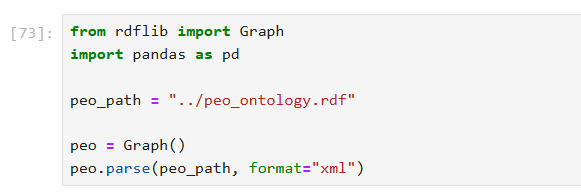
\includegraphics[width=0.9\linewidth]{Figures/fig_45.png}
    \caption{Jupyter notebook SPARQL}
    \label{fig:enter-label}
\end{figure}
The pandas library is used to display query results in data-frames, for query and display I created three support functions: 
\begin{itemize}
    \item \textit{execute\_query:} it takes as input the SPARQL query string and returns a list of results.

    \item \textit{results\_to\_df:} it takes as input as input the list of results ad creates and returns a dataframe with results inside which columns' names are the label names.

    \item \textit{print\_results:} it iterates on the list of results and prints each element.
\end{itemize}
We can see the implementation below:
\begin{figure}[H]
    \centering
    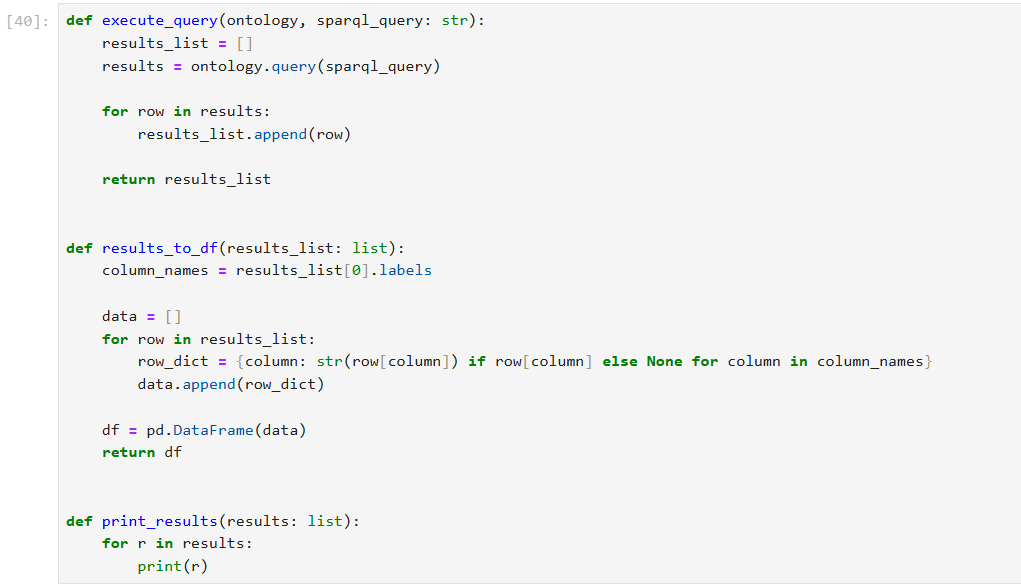
\includegraphics[width=0.9\linewidth]{Figures/fig_46.png}
    \caption{Support python functions}
    \label{fig:enter-label}
\end{figure}
Once this is done, I can translate each of the sixteen competency questions into SPARQL queries to be executed.\\
The first competency question \textbf{CQ1: What is prompt engineering?} is translated into:
\begin{lstlisting}
    SELECT DISTINCT ?property ?value
    WHERE {
        <https://w3id.org/peo#prompt_engineering> ?property ?value .
    }
\end{lstlisting}
Getting the following result:
\begin{figure}[H]
    \centering
    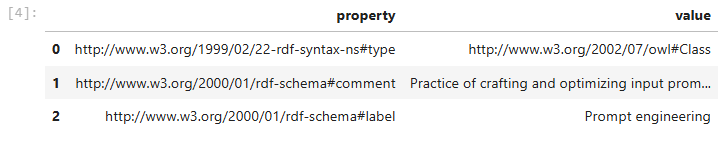
\includegraphics[width=0.9\linewidth]{Figures/fig_47.png}
    \caption{CQ1 SPARQL query results}
    \label{fig:enter-label}
\end{figure}
The output from the query matches the expected result, which is the definition of prompt engineering.\\

The second competency question \textbf{CQ2: What is a prompt?} is translated into:
\begin{lstlisting}
SELECT DISTINCT ?property ?value
WHERE {
    <https://w3id.org/peo#prompt> ?property ?value .
}
\end{lstlisting}
Getting the following results:
\begin{figure}[H]
    \centering
    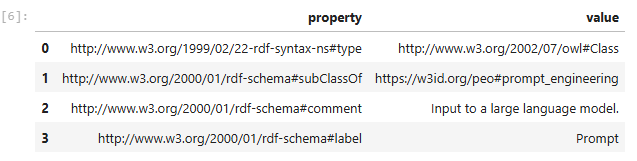
\includegraphics[width=0.9\linewidth]{Figures/fig_48.png}
    \caption{CQ2 SPARQL query results}
    \label{fig:enter-label}
\end{figure}

The output also in this case matches the expected result, which is the definition of prompt.\\

The third competency question \textbf{CQ3: What are prompting techniques?} is translated into:
\begin{lstlisting}
SELECT DISTINCT ?subclass ?label
WHERE {
    ?subclass rdfs:subClassOf <https://w3id.org/peo#prompting_technique> .
    OPTIONAL { ?subclass rdfs:label ?label . }
}
\end{lstlisting}
Getting the following results:
\begin{figure}[H]
    \centering
    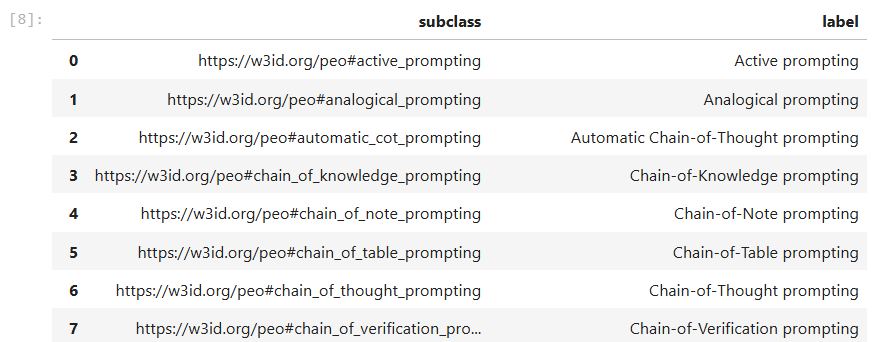
\includegraphics[width=0.9\linewidth]{Figures/fig_49.png}
    \caption{CQ3 SPARQL query results}
    \label{fig:enter-label}
\end{figure}
The complete table contains, as expected, all the prompting techniques in the ontology.\\

The fourth competency question \textbf{CQ4: What are image prompting techniques?} is translated into:
\begin{lstlisting}
SELECT DISTINCT ?subclass ?label
WHERE {
    ?subclass rdfs:subClassOf <https://w3id.org/peo#image_prompting> .
    OPTIONAL { ?subclass rdfs:label ?label . }
}
\end{lstlisting}
Getting the following results:
\begin{figure}[H]
    \centering
    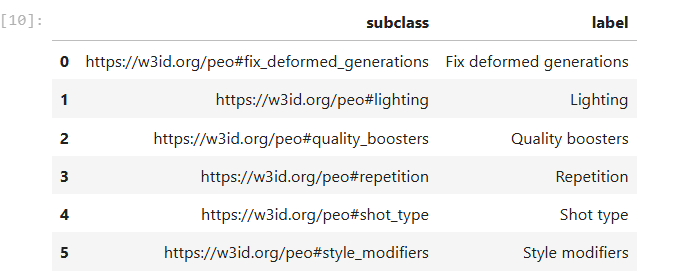
\includegraphics[width=0.9\linewidth]{Figures/fig_50.png}
    \caption{CQ4 SPARQL query results}
    \label{fig:enter-label}
\end{figure}
As expected, we get all the image prompting techniques in the ontology.\\

The fifth competency question \textbf{CQ5: What are code prompting techniques?} is translated into:
\begin{lstlisting}
SELECT DISTINCT ?subclass ?label
WHERE {
    ?subclass rdfs:subClassOf <https://w3id.org/peo#code_prompting> .
    OPTIONAL { ?subclass rdfs:label ?label . }
}  
\end{lstlisting}
Getting the following results:
\begin{figure}[H]
    \centering
    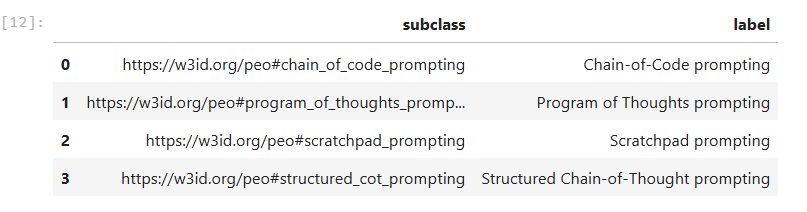
\includegraphics[width=0.9\linewidth]{Figures/fig_51.png}
    \caption{CQ5 SPARQL query results}
    \label{fig:enter-label}
\end{figure}
The table contains, as expected, all the code prompting techniques in the ontology.\\

The sixth competency question \textbf{CQ6: Which task does a prompt solve?} is translated into:
\begin{lstlisting}
SELECT DISTINCT ?prompt ?task ?taskLabel
WHERE {
    ?prompt <https://w3id.org/peo#solves> ?task .
    OPTIONAL { ?task rdfs:label ?taskLabel . }
}
\end{lstlisting}
Getting the following results:
\begin{figure}[H]
    \centering
    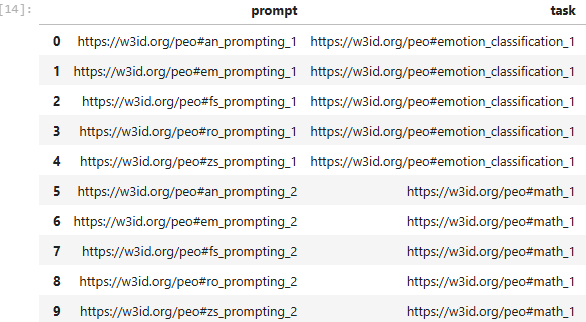
\includegraphics[width=0.9\linewidth]{Figures/fig_52.png}
    \caption{CQ6 SPARQL query results}
    \label{fig:enter-label}
\end{figure}
The table contains, as expected, all the prompts that solve tasks.\\

The seventh competency question \textbf{CQ7: Which prompts are generated using a prompting technique?} is translated into:
\begin{lstlisting}
SELECT DISTINCT ?prompt ?technique ?techniqueLabel
WHERE {
    ?prompt <https://w3id.org/peo#prompt_generated_using> ?technique .
    OPTIONAL { ?technique rdfs:label ?techniqueLabel . }
}
\end{lstlisting}
Getting the following results:
\begin{figure}[H]
    \centering
    \includegraphics[width=0.9\linewidth]{Figures/fig_53.png}
    \caption{CQ7 SPARQL query results}
    \label{fig:enter-label}
\end{figure}
The complete table, as expected, contains all the prompt instances generated using instances of prompting techniques.\\

The eighth competency question \textbf{CQ8: What are the responses that follow each prompt?} is translated into:
\begin{lstlisting}
SELECT DISTINCT ?prompt ?response
WHERE {
    ?response <https://w3id.org/peo#response_followedby_prompt> ?prompt .
}    
\end{lstlisting}
Getting the following results:
\begin{figure}[H]
    \centering
    \includegraphics[width=0.9\linewidth]{Figures/fig_54.png}
    \caption{CQ8 SPARQL query results}
    \label{fig:enter-label}
\end{figure}
The complete table contains, as expected, all the responses of all prompt instances.\\

The ninth competency question \textbf{CQ9: What are possible tasks?} is translated into:
\begin{lstlisting}
SELECT DISTINCT ?task ?label
WHERE {
    ?task rdf:type owl:Class .
    ?task rdfs:subClassOf* <https://w3id.org/peo#task> .
    OPTIONAL { ?task rdfs:label ?label . }
}    
\end{lstlisting}
Getting the following results:
\begin{figure}[H]
    \centering
    \includegraphics[width=0.9\linewidth]{Figures/fig_55.png}
    \caption{CQ9 SPARQL query results}
    \label{fig:enter-label}
\end{figure}
As expected, in the completed table we get all the possible task represented in the ontology.\\

The tenth competency question \textbf{CQ10: Which tasks are related to the text?} is translated into:
\begin{lstlisting}
SELECT DISTINCT ?task ?label
WHERE {
    ?task rdf:type owl:Class .
    ?task rdfs:subClassOf* <https://w3id.org/peo#text_task> .
    OPTIONAL { ?task rdfs:label ?label . }
}
\end{lstlisting}
Getting the following results:
\begin{figure}[H]
    \centering
    \includegraphics[width=0.9\linewidth]{Figures/fig_56.png}
    \caption{CQ10 SPARQL query results}
    \label{fig:enter-label}
\end{figure}

The resulting table, as expected, contains, all the task related to text.\\

The eleventh competency question \textbf{CQ11: What is a chat?} is translated into:
\begin{lstlisting}
SELECT DISTINCT ?property ?value
WHERE {
    <https://w3id.org/peo#chat> ?property ?value .
}
\end{lstlisting}
Getting the following results:
\begin{figure}[H]
    \centering
    \includegraphics[width=0.9\linewidth]{Figures/fig_57.png}
    \caption{CQ11 SPARQL query results}
    \label{fig:enter-label}
\end{figure}
The result, as expected, is the definition of Chat.\\

The twelfth competency question \textbf{CQ12: What is a large language model?} is translated into:
\begin{lstlisting}
SELECT DISTINCT ?property ?value
WHERE {
    <https://w3id.org/peo#large_language_model> ?property ?value .
}
\end{lstlisting}
Getting the following results:
\begin{figure}[H]
    \centering
    \includegraphics[width=0.9\linewidth]{Figures/fig_58.png}
    \caption{CQ12 SPARQL query results}
    \label{fig:enter-label}
\end{figure}
The result, as expected, is the definition of Large Language Model.\\

The thirteenth competency question \textbf{CQ13: What types of large language models are available?} is translated into:
\begin{lstlisting}
SELECT DISTINCT ?type ?label
WHERE {
    ?type rdfs:subClassOf <https://w3id.org/peo#large_language_model> .
    OPTIONAL { ?type rdfs:label ?label . }
}
\end{lstlisting}
Getting the following results:
\begin{figure}[H]
    \centering
    \includegraphics[width=0.9\linewidth]{Figures/fig_59.png}
    \caption{CQ13 SPARQL query results}
    \label{fig:enter-label}
\end{figure}
The resulting complete table, as expected, is the collection of all large language models represented in the ontology.\\

The fourteenth competency question \textbf{CQ14: What are large language models architectures?} is translated into:
\begin{lstlisting}
SELECT DISTINCT ?type ?label
WHERE {
    ?type rdfs:subClassOf <https://w3id.org/peo#base_model> .
    OPTIONAL { ?type rdfs:label ?label . }
}   
\end{lstlisting}
Getting the following results:
\begin{figure}[H]
    \centering
    \includegraphics[width=0.9\linewidth]{Figures/fig_60.png}
    \caption{CQ14 SPARQL query results}
    \label{fig:enter-label}
\end{figure}
The result, as expected, is the collection of main large language models architectures.\\

The fifteenth competency question \textbf{CQ15: What are large language models capabilities?} is translated into:
\begin{lstlisting}
SELECT DISTINCT ?type ?label
WHERE {
    ?type rdfs:subClassOf <https://w3id.org/peo#capability> .
    OPTIONAL { ?type rdfs:label ?label . }
}
\end{lstlisting}
Getting the following results:
\begin{figure}[H]
    \centering
    \includegraphics[width=0.8\linewidth]{Figures/fig_61.png}
    \caption{CQ15 SPARQL query results}
    \label{fig:enter-label}
\end{figure}
As expected, the results is the collection of all the capabilities represented in the ontology.\\

The sixteenth and last competency question \textbf{CQ16: What companies develop large language models?} is translated into:
\begin{lstlisting}
SELECT DISTINCT ?company ?label
WHERE {
    ?company rdf:type <https://w3id.org/peo#company> .
    OPTIONAL { ?company rdfs:label ?label . }
}
\end{lstlisting}
Getting the following results:
\begin{figure}[H]
    \centering
    \includegraphics[width=0.8\linewidth]{Figures/fig_62.png}
    \caption{CQ16 SPARQL query results}
    \label{fig:enter-label}
\end{figure}
The result, as expected, is the collection of companies that develop large language models.


\newpage
\section{Ontology publication and maintenance}
The last step after the Ontology implementation in the LOT methodology is the Ontology publication phase, which scope is to provide an online ontology accessible both as human-readable documentation and a machine-readable documentation from its URI. This phase is divided into three sub-activities:
\begin{enumerate}
    \item \textbf{Propose release candidate}
    \item \textbf{Ontology documentation}
    \item \textbf{Online publication}
\end{enumerate}
as we can see in the figure below:
\begin{figure}[H]
    \centering
    \includegraphics[width=0.9\linewidth]{Figures/fig_25.png}
    \caption{Ontology publication workflow}
    \label{fig:enter-label}
\end{figure}

\subsection{Propose release candidate}
After all the implementation and evaluation, in this step there is the decision about which version of the ontology is going to be published. It is a quite easy choice because, as said in pervious sections, the version populated automatically did not added any useful information from the original version. Moreover it added, according the OOPS! report, more pitfalls (five vs three) so the ontology that is going to be published is the 1.0 version of PEO ontology, populated manually without any llm intervention.
\begin{figure}[H]
    \centering
    \includegraphics[width=0.36\linewidth]{Figures/fig_64.jpg}
    \caption{Ontology version choosing}
    \label{fig:enter-label}
\end{figure}

\subsection{Ontology documentation}
The ontology documentation is generated using Protegé and the OWLdoc plug-in which automatically generate HTML documentation starting from ontology code. The output of OWLdoc is the following:
\begin{figure}[H]
    \centering
    \includegraphics[width=0.9\linewidth]{Figures/fig_63.png}
    \caption{OWLdoc output}
    \label{fig:enter-label}
\end{figure}
The OWLdoc is available in the Github repository \href{https://github.com/simonegramegna/peo/tree/main/docs}{here} in the \textit{/docs} folder and it can be consulted online \href{https://peoontology.vercel.app/}{here}. The documentation is made accessible for everyone using Vercel: a cloud platform for hosting web applications and static sites. This free service using an integrated Github action, takes as input the documentation in the repository and publishes online automatically without requiring any effort by the developer. The \textit{official documentation website} is:
\href{https://peoontology.vercel.app/}{https://peoontology.vercel.app/}.

\subsection{Online publication}
Once the ontology documentation is ready, the ontology can be published online on major vocabularies repository, by accessing the ontology using its URI. I will consider two most known repositories for ontology publishing: \href{https://w3id.org/}{w3id.org} and \href{https://bioportal.bioontology.org/}{BioPortal}.

\subsubsection{W3id.org}
W3id.org a permanent identifier service that provides stable, persistent, and HTTP-resolvable URIs for web resource. The creation of a new identifier for publishing a new ontology is made using Github and the official W3id.org Github repository. The procedure followed is straightforward, first I fork the W3id.org Github repository on my Github, creating a "copy" of the repository. 
\begin{figure}[H]
    \centering
    \includegraphics[width=0.9\linewidth]{Figures/fig_65.png}
    \caption{Forked W3id.org repository}
    \label{fig:enter-label}
\end{figure}
Then I create a new branch and I create a new directory with the intended permanent identifier name, in my case I create a directory called \textit{"peo"}. Inside this directory I create two files:
\begin{itemize}
    \item \textit{README.md:} contains more identifier info and contact info, for human to read.
    \item \textit{.htaccess:} contains redirection rules, for computer to read and perform.
\end{itemize}
In the case of PEO ontology, the \textit{README.md} contains all my contact information with the link to the peo Github repository while the \textit{.htaccess} contains the following redirections rules:
\begin{lstlisting}
# Activates Rewrite Engine
RewriteEngine On

# Content negotiation for RDF/XML
RewriteCond %{HTTP_ACCEPT} application/rdf\+xml
RewriteRule ^$ https://raw.githubusercontent.com/simonegramegna/peo/refs/heads/main/peo_ontology.rdf [R=303,L]

# Content negotiation for Turtle
RewriteCond %{HTTP_ACCEPT} text/turtle
RewriteRule ^$ https://raw.githubusercontent.com/simonegramegna/peo/refs/heads/main/peo_ontology.ttl [R=303,L]

# Default: serves HTML for browser or client not RDF-aware
RewriteRule ^$ https://peoontology.vercel.app/ [R=303,L]

# Blocks directory indexing
Options -Indexes
\end{lstlisting}
Once the two files are completed, I submitted a pull request to the main branch that is approved by one of repository administrators. As soon the merge of the created branch, it is possible to access to the ontology using its URI, in the case of PEO ontology the URI is: \href{https://w3id.org/peo}{https://w3id.org/peo} bringing the user with an HTTP request to the online ontology documentation.
\begin{figure}[H]
    \centering
    \includegraphics[width=0.9\linewidth]{Figures/fig_66.png}
    \caption{W3id.org repository main directory}
    \label{fig:enter-label}
\end{figure}

\subsubsection{BioPortal}
BioPortal is a  web-based platform designed for the management, exploration, and publication of biomedical ontologies, during the years it has become popular among ontology engineers choosing it as a repository for the publication of different types of ontologies not only in biomedical field. BioPortal offers developers a simple and intuitive interface to publish an ontology, providing the ability to track various versions and visits to the ontology. First I created an account on BioPortal and then I specified all the informations about the ontology: the version, the type (RDF) and the release date. I also specified my contact informations like the e-mail and the Github repository.
\begin{figure}[H]
    \centering
    \includegraphics[width=0.9\linewidth]{Figures/fig_67.png}
    \caption{BioPortal main page}
    \label{fig:enter-label}
\end{figure}
The ontology is published at the link \href{https://bioportal.bioontology.org/ontologies/PEO_ONTOLOGY?p=summary}{here} and it is possible using the web interface view the whole ontology: classes, object properties, data properties and individuals. This is a very useful feature because the user has no need to download any additional software, moreover BioPortal computes automatically base ontology metrics. 
\begin{figure}[H]
    \centering
    \includegraphics[width=0.9\linewidth]{Figures/fig_68.png}
    \caption{BioPortal ontology interface}
    \label{fig:enter-label}
\end{figure}


\newpage
\section{Ontology maintenance}
The ontology maintenance is the phase that concludes the iteration of the ontology development process, the goal of this phase is to update the ontology during its life cycle. This phase in the case of prompt engineering ontology is important, prompting techniques and large language models are constantly evolving, and regularly updating the ontology is essential to keep it aligned with the latest technologies introduced.\\
In cases where the necessary changes significantly alter the structure of the ontology, it is advisable to formulate new functional requirements through updated competency questions that align with the changes to be introduced. Changes may lead not only to updates but also to the introduction of bugs and pitfalls, which can be identified through the evaluation techniques previously discussed and resolving these issues ensures the quality of the ontology. In general, monitoring and maintaining the traceability of the requirements, bugs and suggestions identified in this activity allows storing discussions and decisions taken that can be later reused. The LOT methodology is designed to support those practices aligned with modern software engineering methodology like the agile methodology from whose iterativity it draws inspiration.

\begin{figure}[H]
    \centering
    \includegraphics[width=0.9\linewidth]{Figures/fig_33.png}
    \caption{Ontology maintenance workflow}
    \label{fig:enter-label}
\end{figure}

\newpage
\section{Results discussion}








\chapter{Ontology evaluation}
\label{chapter:5_evaluation}

\section{Ontology consistency check}
\label{subsection:5_1_evaluation}
The ontology consistency check consists in running the reasoner in order to check the consistency of declared and inferenced classes and axioms, inferences are made using also SWRL rules described in the encoding section. Running the reasoner ensures also the declaration of disjointness among disjoint classes. I run the HermiT reasoner on both version of the PEO: the version populated manually and the updated version made by GPT-4.\\
On the original version of the PEO, the reasoner does not give any inconsistency and all the axioms are inferred correctly.
\begin{figure}[H]
    \centering
    \includegraphics[width=0.9\linewidth]{Figures/fig_39.png}
    \caption{PEO with HermiT reasoner}
    \label{fig:39}
\end{figure}
The Fig. \ref{fig:39} shows the execution of HermiT reasoner on PEO.
The reasoner infers correctly that the class "Alpaca" is disjoint with the classes "Task", "Base model", "Prompt engineering", "Organization" and "Capability" because the superclass "Large language model" is declared disjoint with that list of classes. The ten SWRL rules declared work properly and inference the correct object properties for individuals:
\begin{figure}[H]
    \centering
    \includegraphics[width=0.9\linewidth]{Figures/fig_40.png}
    \caption{Inference on prompt individual}
    \label{fig:40}
\end{figure}
The consistency check of the other version of the PEO, the one populated using GPT-4 has given the exact results, this because as said in the previous section no additional significant information has been added to the ontology. The inserted classes have no link with other classes so there are no other new inferences.

\subsection{OntoMetrics}
\label{subsection:4_4_2_ontometrics}
The calculation of metrics is done using OntoMetrics: a web-based tool developed by the University of Rostock that validates and provides statistical analyses of ontologies.\cite{lantow2016ontometrics}
Given the ontology in form of RDF file or code, it calculates automatically:
\begin{itemize}
    \item Base metrics: these include simple counts of ontology elements such as classes, axioms, and objects, providing a quantitative overview of the ontology's components.

    \item Schema Metrics: these metrics evaluate the structure of the ontology's schema, considering aspects like attribute richness and inheritance richness.

    \item Knowledge base Metrics: these assess the ontology's knowledge base, focusing on the population of instances within the ontology.

    \item Class Metrics: these metrics analyse individual classes within the ontology, examining factors such as class connectivity and fullness.

    \item Graph Metrics: these evaluate the ontology's taxonomy as a graph, measuring properties like depth and breadth.
\end{itemize}
For PEO, I will calculate base metrics, schema metrics and graph metrics.
\begin{figure}[H]
    \centering
    \includegraphics[width=0.9\linewidth]{Figures/fig_41.png}
    \caption{OntoMetrics interface}
    \label{fig:enter-label}
\end{figure}

Values computed for \textbf{base metrics} are:

\begin{table}[H]
    \centering
    \begin{tabular}{|>{\raggedright\arraybackslash}p{8cm}|>{\raggedright\arraybackslash}p{4cm}|}
        \hline
        \textbf{Property} & \textbf{Value} \\ \hline
        Axioms & 2684 \\ \hline
        Logical axioms count & 1695 \\ \hline
        Class count & 126 \\ \hline
        Total classes count & 126 \\ \hline
        Object property count & 34 \\ \hline
        Total object properties count & 34 \\ \hline
        Data property count & 13 \\ \hline
        Total data properties count & 13 \\ \hline
        Properties count & 47 \\ \hline
        Individual count & 352 \\ \hline
        Total individuals count & 352 \\ \hline
        DL expressivity & SRIF(D) \\ \hline
    \end{tabular}
    \caption{PEO base metrics statistics}
    \label{tab:ontology-stats}
\end{table}
This table provides a high-level overview of the ontology’s structure and complexity. With 2684 axioms, the ontology is rich in detail and represents a substantial body of knowledge. Among these, 1695 logical axioms indicate a strong focus on enabling inference and reasoning. The 126 classes show that the ontology has a robust framework for organizing concepts, while 34 object properties and 13 data properties highlight the ontology’s emphasis on relationships over attribute-driven modeling. The inclusion of 352 individuals suggests that the ontology is well-populated, demonstrating practical applicability. The expressivity of SRIF(D) indicates that the ontology supports features like inverse roles and data ranges, balancing computational efficiency with expressive capability. This ontology is comprehensive but may require optimization to handle its inherent complexity effectively.

\begin{table}[H]
    \centering
    \begin{tabular}{|>{\raggedright\arraybackslash}p{8cm}|>{\raggedright\arraybackslash}p{4cm}|}
        \hline
        \textbf{Class Axiom Type} & \textbf{Count} \\ \hline
        SubClassOf axioms count & 199 \\ \hline
        Equivalent classes axioms count & 1 \\ \hline
        Disjoint classes axioms count & 3 \\ \hline
        GCICount & 0 \\ \hline
        HiddenGCICount & 0 \\ \hline
    \end{tabular}
    \caption{PEO Class Axioms statistics}
    \label{tab:class-axioms}
\end{table}

This table details how classes are defined and interrelated within the ontology. The 199 SubClassOf axioms form a strong hierarchical backbone, enabling inheritance of properties and constraints. However, the limited use of equivalent classes (1) and disjoint classes (3) suggests that the ontology may not fully capture nuanced relationships or enforce strict separations between certain concepts. The absence of GCIs (Global Cardinality Restrictions) and Hidden GCIs could indicate missed opportunities to model constraints and relationships that extend across the ontology as a whole. While the current setup simplifies reasoning, incorporating more advanced axioms could enhance the ontology's semantic richness and utility.


\begin{table}[H]
    \centering
    \begin{tabular}{|>{\raggedright\arraybackslash}p{8cm}|>{\raggedright\arraybackslash}p{4cm}|}
        \hline
        \textbf{Object Property Axiom Type} & \textbf{Count} \\ \hline
        SubObjectPropertyOf axioms count & 33 \\ \hline
        Equivalent object properties axioms count & 0 \\ \hline
        Inverse object properties axioms count & 16 \\ \hline
        Disjoint object properties axioms count & 0 \\ \hline
        Functional object properties axioms count & 0 \\ \hline
        Inverse functional object properties axioms count & 0 \\ \hline
        Transitive object property axioms count & 2 \\ \hline
        Symmetric object property axioms count & 0 \\ \hline
        Asymmetric object property axioms count & 0 \\ \hline
        Reflexive object property axioms count & 0 \\ \hline
        Irreflexive object property axioms count & 1 \\ \hline
        Object property domain axioms count & 33 \\ \hline
        Object property range axioms count & 33 \\ \hline
        SubPropertyChainOf axioms count & 0 \\ \hline
    \end{tabular}
    \caption{PEO Object Property Axioms Statistics}
    \label{tab:object-property-axioms}
\end{table}
Object properties are the backbone of the ontology's relational structure. With 33 SubObjectPropertyOf axioms, the ontology defines a clear hierarchy of relationships, which helps maintain organization and reasoning efficiency. The 16 inverse object properties highlight a good use of bidirectional relationships, enhancing navigability within the graph. However, the lack of functional, inverse functional, symmetric, or asymmetric properties may limit the ontology’s ability to capture specific constraints, such as unique or one-to-one relationships. The two transitive properties and one irreflexive property add some complexity but are underused. Domains and ranges are well-defined for all object properties, which is a strong point, as it ensures consistency and logical soundness in property usage.

\begin{table}[H]
    \centering
    \begin{tabular}{|>{\raggedright\arraybackslash}p{8cm}|>{\raggedright\arraybackslash}p{4cm}|}
        \hline
        \textbf{Data Property Axiom Type} & \textbf{Count} \\ \hline
        SubDataPropertyOf axioms count & 12 \\ \hline
        Equivalent data properties axioms count & 0 \\ \hline
        Disjoint data properties axioms count & 0 \\ \hline
        Functional data property axioms count & 7 \\ \hline
        Data property domain axioms count & 11 \\ \hline
        Data property range axioms count & 12 \\ \hline
    \end{tabular}
    \caption{PEO Data Property Axioms Statistics}
    \label{tab:data-property-axioms}
\end{table}

Data properties focus on attributes of individuals. The 12 SubDataPropertyOf axioms indicate some level of organization, but the absence of equivalent or disjoint data properties suggests limited semantic relationships among these properties. Seven functional data properties point to a partial emphasis on ensuring that certain attributes have unique values (e.g., “hasID”), but this aspect could be expanded. Domains and ranges are defined for most properties, which improves clarity and reasoning, but the relatively low overall count of data property axioms might limit the ontology's ability to model detailed attributes of classes or individuals.

\begin{table}[H]
    \centering
    \begin{tabular}{|>{\raggedright\arraybackslash}p{8cm}|>{\raggedright\arraybackslash}p{4cm}|}
        \hline
        \textbf{Individual Axiom Type} & \textbf{Count} \\ \hline
        Class assertion axioms count & 352 \\ \hline
        Object property assertion axioms count & 390 \\ \hline
        Data property assertion axioms count & 580 \\ \hline
        Negative object property assertion axioms count & 0 \\ \hline
        Negative data property assertion axioms count & 0 \\ \hline
        Same individuals axioms count & 0 \\ \hline
        Different individuals axioms count & 0 \\ \hline
    \end{tabular}
    \caption{PEO Individual Axioms Statistics}
    \label{tab:individual-axioms}
\end{table}

This table reflects how individuals are represented and connected within the ontology. The 352 class assertions and 390 object property assertions indicate that the ontology’s individuals are well-categorized and interlinked. The 580 data property assertions further show that these individuals have descriptive attributes. However, the absence of negative assertions (both object and data properties) and no axioms for declaring individuals as equivalent or distinct may limit the ontology's ability to handle complex scenarios, such as resolving conflicts or managing redundancy.

\begin{table}[H]
    \centering
    \begin{tabular}{|>{\raggedright\arraybackslash}p{8cm}|>{\raggedright\arraybackslash}p{4cm}|}
        \hline
        \textbf{Annotation Axiom Type} & \textbf{Count} \\ \hline
        Annotation axioms count & 5 \\ \hline
        Annotation assertion axioms count & 459 \\ \hline
        Annotation property domain axioms count & 0 \\ \hline
        Annotation property range axioms count & 0 \\ \hline
    \end{tabular}
    \caption{PEO Annotation Axioms Statistics}
    \label{tab:annotation-axioms}
\end{table}
Annotations are crucial for documentation and understanding. With 459 annotation assertions, the ontology appears well-documented, providing metadata that can improve usability and comprehension. However, the absence of domain and range axioms for annotation properties suggests that these annotations are not constrained formally, which could lead to inconsistencies or reduced clarity in large-scale applications. Better structuring of annotation properties could enhance the ontology’s maintainability.\\
The \textbf{Schema metrics} computed for PEO are: 

\begin{table}[H]
    \centering
    \begin{tabular}{|>{\raggedright\arraybackslash}p{8cm}|>{\raggedright\arraybackslash}p{4cm}|}
        \hline
        \textbf{Metric} & \textbf{Value} \\ \hline
        Attribute richness & 0.103175 \\ \hline
        Inheritance richness & 1.579365 \\ \hline
        Relationship richness & 0.160338 \\ \hline
        Attribute class ratio & 0.0 \\ \hline
        Equivalence ratio & 0.007937 \\ \hline
        Axiom/class ratio & 21.301587 \\ \hline
        Inverse relations ratio & 0.390244 \\ \hline
        Class/relation ratio & 0.531646 \\ \hline
    \end{tabular}
    \caption{PEO Schema Metrics}
    \label{tab:ontology-metrics}
\end{table}
This table evaluates the structural aspects of the ontology. The attribute richness (0.103175) indicates that relatively few classes have associated attributes, which could limit the detail available for each class. The inheritance richness (1.579365) shows that most classes are part of meaningful hierarchies, a positive sign of structure. However, the relationship richness (0.160338) is relatively low, suggesting that the ontology focuses more on defining concepts than on interconnecting them. The axiom-to-class ratio (21.301587) highlights a dense ontology, meaning each class has substantial associated information, which can be both a strength and a source of complexity. Finally, the inverse relations ratio (0.390244) indicates a good but incomplete use of inverse properties to enhance navigability.\\
The \textbf{Graph metrics} for PEO are:
\begin{table}[H]
    \centering
    \begin{tabular}{|>{\raggedright\arraybackslash}p{8cm}|>{\raggedright\arraybackslash}p{4cm}|}
        \hline
        \textbf{Metric} & \textbf{Value} \\ \hline
        Absolute root cardinality & 7 \\ \hline
        Absolute leaf cardinality & 109 \\ \hline
        Absolute sibling cardinality & 126 \\ \hline
        Absolute depth & 318 \\ \hline
        Average depth & 2.52381 \\ \hline
        Maximal depth & 4 \\ \hline
        Absolute breadth & 126 \\ \hline
        Average breadth & 7.0 \\ \hline
        Maximal breadth & 33 \\ \hline
        Ratio of leaf fan-outness & 0.865079 \\ \hline
        Ratio of sibling fan-outness & 1.0 \\ \hline
        Tangledness & 0.269841 \\ \hline
        Total number of paths & 126 \\ \hline
        Average number of paths & 31.5 \\ \hline
    \end{tabular}
    \caption{PEO Graph Metrics}
    \label{tab:cardinality-depth-metrics}
\end{table}
Graph metrics provide insights into the topology of the ontology. The absolute root cardinality (7) and absolute leaf cardinality (109) indicate a moderately deep hierarchy with good granularity at the leaf level. The maximal depth (4) and average depth (2.52381) suggest a shallow graph, which can make the ontology easier to understand but may oversimplify complex domains. The tangledness (0.269841) is moderate, indicating a graph structure that is connected but not overly complex. The high sibling fan-out ratio (1.0) shows that sibling classes are evenly distributed, while the ratio of leaf fan-outness (0.865079) implies a balanced spread of subclasses from intermediate nodes.\\
Despite there being no significant differences between the original version of the PEO and the version populated using GPT-4, I proceed to calculate metrics.\\
Values computed for base metrics are:
\begin{table}[H]
    \centering
    \begin{tabular}{|>{\raggedright\arraybackslash}p{8cm}|>{\raggedright\arraybackslash}p{4cm}|}
        \hline
        \textbf{Property} & \textbf{Value} \\ \hline
        Axioms & 2705 \\ \hline
        Logical axioms count & 1710 \\ \hline
        Class count & 128 \\ \hline
        Total classes count & 128 \\ \hline
        Object property count & 34 \\ \hline
        Total object properties count & 34 \\ \hline
        Data property count & 13 \\ \hline
        Total data properties count & 13 \\ \hline
        Properties count & 47 \\ \hline
        Individual count & 359 \\ \hline
        Total individuals count & 359 \\ \hline
        DL expressivity & SRIF(D) \\ \hline
    \end{tabular}
    \caption{PEO updated base metrics statistics}
    \label{tab:ontology-stats-updated}
\end{table}

\begin{table}[H]
    \centering
    \begin{tabular}{|>{\raggedright\arraybackslash}p{8cm}|>{\raggedright\arraybackslash}p{4cm}|}
        \hline
        \textbf{Class Axiom Type} & \textbf{Count} \\ \hline
        SubClassOf axioms count & 197 \\ \hline
        Equivalent classes axioms count & 1 \\ \hline
        Disjoint classes axioms count & 3 \\ \hline
        GCICount & 0 \\ \hline
        HiddenGCICount & 0 \\ \hline
    \end{tabular}
    \caption{PEO updated Class Axioms Statistics}
    \label{tab:class-axioms-updated}
\end{table}

\begin{table}[H]
    \centering
    \begin{tabular}{|>{\raggedright\arraybackslash}p{8cm}|>{\raggedright\arraybackslash}p{4cm}|}
        \hline
        \textbf{Object Property Axiom Type} & \textbf{Count} \\ \hline
        SubObjectPropertyOf axioms count & 33 \\ \hline
        Equivalent object properties axioms count & 0 \\ \hline
        Inverse object properties axioms count & 16 \\ \hline
        Disjoint object properties axioms count & 0 \\ \hline
        Functional object properties axioms count & 0 \\ \hline
        Inverse functional object properties axioms count & 0 \\ \hline
        Transitive object property axioms count & 8 \\ \hline
        Symmetric object property axioms count & 1 \\ \hline
        Asymmetric object property axioms count & 0 \\ \hline
        Reflexive object property axioms count & 0 \\ \hline
        Irreflexive object property axioms count & 1 \\ \hline
        Object property domain axioms count & 33 \\ \hline
        Object property range axioms count & 33 \\ \hline
        SubPropertyChainOf axioms count & 0 \\ \hline
    \end{tabular}
    \caption{PEO updated Object Property Axioms Statistics}
    \label{tab:object-property-axioms-updated}
\end{table}

\begin{table}[H]
    \centering
    \begin{tabular}{|>{\raggedright\arraybackslash}p{8cm}|>{\raggedright\arraybackslash}p{4cm}|}
        \hline
        \textbf{Data Property Axiom Type} & \textbf{Count} \\ \hline
        SubDataPropertyOf axioms count & 12 \\ \hline
        Equivalent data properties axioms count & 0 \\ \hline
        Disjoint data properties axioms count & 0 \\ \hline
        Functional data property axioms count & 7 \\ \hline
        Data property domain axioms count & 12 \\ \hline
        Data property range axioms count & 12 \\ \hline
    \end{tabular}
    \caption{PEO updated Data Property Axioms Statistics}
    \label{tab:data-property-axioms-updated}
\end{table}

\begin{table}[H]
    \centering
    \begin{tabular}{|>{\raggedright\arraybackslash}p{8cm}|>{\raggedright\arraybackslash}p{4cm}|}
        \hline
        \textbf{Individual Axiom Type} & \textbf{Count} \\ \hline
        Class assertion axioms count & 358 \\ \hline
        Object property assertion axioms count & 393 \\ \hline
        Data property assertion axioms count & 580 \\ \hline
        Negative object property assertion axioms count & 0 \\ \hline
        Negative data property assertion axioms count & 0 \\ \hline
        Same individuals axioms count & 0 \\ \hline
        Different individuals axioms count & 0 \\ \hline
    \end{tabular}
    \caption{PEO updated Individual Axioms Statistics}
    \label{tab:individual-axioms-updated}
\end{table}

\begin{table}[H]
    \centering
    \begin{tabular}{|>{\raggedright\arraybackslash}p{8cm}|>{\raggedright\arraybackslash}p{4cm}|}
        \hline
        \textbf{Annotation Axiom Type} & \textbf{Count} \\ \hline
        Annotation axioms count & 5 \\ \hline
        Annotation assertion axioms count & 456 \\ \hline
        Annotation property domain axioms count & 0 \\ \hline
        Annotation property range axioms count & 0 \\ \hline
    \end{tabular}
    \caption{PEO updated Annotation Axioms Statistics}
    \label{tab:annotation-axioms-updated}
\end{table}

The schema metrics for the update version of PEO are:
\begin{table}[H]
    \centering
    \begin{tabular}{|>{\raggedright\arraybackslash}p{8cm}|>{\raggedright\arraybackslash}p{4cm}|}
        \hline
        \textbf{Metric} & \textbf{Value} \\ \hline
        Attribute richness & 0.101563 \\ \hline
        Inheritance richness & 1.539063 \\ \hline
        Relationship richness & 0.161702 \\ \hline
        Attribute class ratio & 0.0 \\ \hline
        Equivalence ratio & 0.007813 \\ \hline
        Axiom/class ratio & 21.132813 \\ \hline
        Inverse relations ratio & 0.390244 \\ \hline
        Class/relation ratio & 0.544681 \\ \hline
    \end{tabular}
    \caption{PEO Schema Metrics}
    \label{tab:ontology-metrics-updated}
\end{table}

The graph metrics for updated version of PEO are:

\begin{table}[H]
    \centering
    \begin{tabular}{|>{\raggedright\arraybackslash}p{8cm}|>{\raggedright\arraybackslash}p{4cm}|}
        \hline
        \textbf{Metric} & \textbf{Value} \\ \hline
        Absolute root cardinality & 11 \\ \hline
        Absolute leaf cardinality & 111 \\ \hline
        Absolute sibling cardinality & 128 \\ \hline
        Absolute depth & 316 \\ \hline
        Average depth & 2.46875 \\ \hline
        Maximal depth & 4 \\ \hline
        Absolute breadth & 128 \\ \hline
        Average breadth & 7.111111 \\ \hline
        Maximal breadth & 33 \\ \hline
        Ratio of leaf fan-outness & 0.867188 \\ \hline
        Ratio of sibling fan-outness & 1.0 \\ \hline
        Tangledness & 0.265625 \\ \hline
        Total number of paths & 128 \\ \hline
        Average number of paths & 32.0 \\ \hline
    \end{tabular}
    \caption{PEO updated Graph Metrics}
    \label{tab:cardinality-depth-metrics-updated}
\end{table}
The new values calculated by OntoMetrics on the updated version of the ontology do not differ significantly from the previously calculated values, as the large language model GPT-4 has only added four new classes and three new instances. All results for PEO and its second version are on \href{https://github.com/simonegramegna/peo/tree/main/evaluation}{Github}.

\newpage
\subsection{OOPS! validation}
\label{subsection:4_4_3_oops}
The methods discussed so far are widely used in ontology evaluation; however, they are not capable of capturing modelling errors in greater detail. These errors can compromise not only the quality and usability of the ontology but also lead to potential inconsistencies. Therefore, it is necessary to adopt a different approach from those previously examined, OntoMetrics and the HermiT reasoner because they have the following issues:
\begin{itemize}
    \item OntoMetrics: it provides a quantitative measure of ontology's structural characteristics without analysing qualitative aspects, so it is not able to detect semantic and usability issues in the ontology.

    \item HermiT reasoner (reasoners in general): reasoners are designed to check the logical consistency of an ontology and perform inferencing identifying inconsistencies in axioms. But reasoners are not able to detect errors outside logical inconsistencies, such as missing domain or range definitions and they cannot check best-practice violation and usability issues.
\end{itemize}
These limitations highlight the need for a tool that can go beyond structural and logical evaluation, addressing both semantic and usability dimensions of ontology quality. \textbf{OOPS!} (Ontology Pitfall Scanner) is an online tool for ontology evaluation \cite{poveda2014oops} that automates the evaluation process without requiring any effort by the developer. 
\begin{figure}[H]
    \centering
    \includegraphics[width=0.9\linewidth]{Figures/fig_42.png}
    \caption{OOPS! web interface}
    \label{fig:enter-label}
\end{figure}
Given the input ontology, OOPS is able to detect 40 different pitfall that are classified into three categories: critical, important and minor by parsing the RDF code and generating a complete response using the OOPS! scanner. Pitfalls in the scanner include:
\begin{itemize}
    \item Structural pitfalls: these involve issues related to the ontology's formal structure and syntax like cycles in hierarchy and unconnected ontology elements.

    \item Functional pitfalls: these involve issues to the intended use and functionality of the ontology like missing domain or incorrectly defined inverse relationships.

    \item Usability and Profiling Pitfalls: these involve issues  affecting the ontology's clarity, maintainability, and human-readability like missing annotations, inconsistent naming and ambiguous terms.
\end{itemize}
I will use OOPS! scanner on both versions of the PEO detecting and explaining found pitfalls. 
For the first version of PEO there are just three pitfalls:
\begin{figure}[H]
    \centering
    \includegraphics[width=0.9\linewidth]{Figures/fig_43.png}
    \caption{Detected pitfalls PEO}
    \label{fig:enter-label}
\end{figure}
The explanation of detected pitfall is:
\begin{itemize}
    \item \textbf{P04 (Creating unconnected ontology elements):} this pitfall involves ontology elements (classes, object properties and datatype properties) are created isolated, with no relation to the rest of the ontology. 

    \item \textbf{P34 (Untyped class):} this pitfalls involves all ontology elements that are used as a class without having explicitly declared. This pitfall involves four elements in PEO: \\ \textit{http://www.w3.org/2003/11/swrl\#IndividualPropertyAtom},\\ \textit{http://www.w3.org/2003/11/swrl\#Variable},\\ \textit{http://www.w3.org/2003/11/swrl\#Imp} and \\\textit{http://www.w3.org/2003/11/swrl\#AtomList}.

    \item \textbf{P41 (No license declared):} there is no license in the ontology metadata.    
\end{itemize}
Overall, the report is satisfactory, as no critical pitfalls have been identified, nor any issues found in the main classes or object properties of the ontology and I will discuss in more detail in Results discussion section. The complete report is available \href{https://github.com/simonegramegna/peo/blob/main/evaluation/oops_report_peo.xml}{here}. After detecting pitfalls in the original version of the PEO, I also examined the populated version generated using GPT-4 nonetheless, no significant differences were observed between the two versions. Compared to the three pitfalls identified in the previous version, OOPS detects five pitfalls:
\begin{figure}[H]
    \centering
    \includegraphics[width=0.75\linewidth]{Figures/fig_44.png}
    \caption{Detected pitfalls second version PEO}
    \label{fig:enter-label}
\end{figure}


\begin{itemize}
    \item \textbf{P04 (Creating unconnected ontology elements):} this pitfall, as said before, involves unconnected ontology elements. This time the pitfall involves not only the \textit{prompt\_engineering} class but also the new classes created by GPT-4: \textit{Task}, \textit{PromptingTechnique}, \textit{Prompt} and \textit{PromptEngineering}. Those classes have no relations with other classes.

    \item \textbf{P08 (Missing annotations):} this pitfall involves elements that lack annotation properties that label them ( \textit{rdfs:label}) or that define them\\ (\textit{rdfs:comment}). This pitall involves the four classes created by GPT-4 with no comment provided: \textit{Task}, \textit{PromptingTechnique}, \textit{Prompt} and \textit{PromptEngineering}.  

    \item \textbf{P22 (Using different naming conventions in the ontology):} this pitfall involves ontology elements are not named following the same convention (for example CamelCase or use of delimiters as "-" or "\_"). This pitfall is given by the new classes created by GPT-4 that do not follow the naming convention used in the ontology (with the "\_" separator) by creating classes declared in camel case.

    \item \textbf{P34 (Untyped class):} this is the same pitfall detected before.

    \item \textbf{P41 (No license declared):} this is the same pitfall detected before.
\end{itemize}
In general, the detected pitfalls are caused by GPT-4's lack of understanding of the ontology's structure and I will discuss in more detail in the Results discussion section. The oops report is available \href{https://github.com/simonegramegna/peo/blob/main/evaluation/oops_report_peo_gpt4.xml}{here}.


\subsection{SPARQL queries}
\label{subsection:4_4_4_sparql}
The final step of ontology evaluation is converting competency questions (CQ) defined in the \textit{Ontology requirements specification} section into SPARQL queries in order to compare the expected result to the actual result of each competency question. SPARQL queries are generated manually and ran using Jupyter notebook \cite{jupyter}: an enviroment for running python code and the rdflib python library \cite{rdflib}: a library to access rdf files and run SPARQL queries inside python. The code is available on the \href{https://github.com/simonegramegna/peo/tree/main/evaluation}{Github repository} and the evaluation is mode for both versions of the ontology.\\
First I open the ontology using rdflib:
\begin{figure}[H]
    \centering
    \includegraphics[width=0.9\linewidth]{Figures/fig_45.png}
    \caption{Jupyter notebook SPARQL}
    \label{fig:enter-label}
\end{figure}
The pandas library is used to display query results in data-frames, for query and display I created three support functions: 
\begin{itemize}
    \item \textit{execute\_query:} it takes as input the SPARQL query string and returns a list of results.

    \item \textit{results\_to\_df:} it takes as input as input the list of results ad creates and returns a dataframe with results inside which columns' names are the label names.

    \item \textit{print\_results:} it iterates on the list of results and prints each element.
\end{itemize}
We can see the implementation below:
\begin{figure}[H]
    \centering
    \includegraphics[width=0.9\linewidth]{Figures/fig_46.png}
    \caption{Support python functions}
    \label{fig:enter-label}
\end{figure}

Once this is done, I can translate each of the sixteen competency questions into SPARQL queries to be executed on PEO.\\
The first competency question \textbf{CQ1: What is prompt engineering?} is translated into:
\begin{lstlisting}
    SELECT DISTINCT ?property ?value
    WHERE {
        <https://w3id.org/peo#prompt_engineering> ?property ?value .
    }
\end{lstlisting}
Getting the following result:
\begin{figure}[H]
    \centering
    \includegraphics[width=0.9\linewidth]{Figures/fig_47.png}
    \caption{CQ1 SPARQL query results}
    \label{fig:enter-label}
\end{figure}
The output from the query matches the expected result, which is the definition of prompt engineering.\\

The second competency question \textbf{CQ2: What is a prompt?} is translated into:
\begin{lstlisting}
SELECT DISTINCT ?property ?value
WHERE {
    <https://w3id.org/peo#prompt> ?property ?value .
}
\end{lstlisting}
Getting the following results:
\begin{figure}[H]
    \centering
    \includegraphics[width=0.9\linewidth]{Figures/fig_48.png}
    \caption{CQ2 SPARQL query results}
    \label{fig:enter-label}
\end{figure}

The output also in this case matches the expected result, which is the definition of prompt.\\

The third competency question \textbf{CQ3: What are prompting techniques?} is translated into:
\begin{lstlisting}
SELECT DISTINCT ?subclass ?label
WHERE {
    ?subclass rdfs:subClassOf <https://w3id.org/peo#prompting_technique> .
    OPTIONAL { ?subclass rdfs:label ?label . }
}
\end{lstlisting}
Getting the following results:
\begin{figure}[H]
    \centering
    \includegraphics[width=0.9\linewidth]{Figures/fig_49.png}
    \caption{CQ3 SPARQL query results}
    \label{fig:enter-label}
\end{figure}
The complete table contains, as expected, all the prompting techniques in the ontology.\\

The fourth competency question \textbf{CQ4: What are image prompting techniques?} is translated into:
\begin{lstlisting}
SELECT DISTINCT ?subclass ?label
WHERE {
    ?subclass rdfs:subClassOf <https://w3id.org/peo#image_prompting> .
    OPTIONAL { ?subclass rdfs:label ?label . }
}
\end{lstlisting}
Getting the following results:
\begin{figure}[H]
    \centering
    \includegraphics[width=0.9\linewidth]{Figures/fig_50.png}
    \caption{CQ4 SPARQL query results}
    \label{fig:enter-label}
\end{figure}
As expected, we get all the image prompting techniques in the ontology.\\

The fifth competency question \textbf{CQ5: What are code prompting techniques?} is translated into:
\begin{lstlisting}
SELECT DISTINCT ?subclass ?label
WHERE {
    ?subclass rdfs:subClassOf <https://w3id.org/peo#code_prompting> .
    OPTIONAL { ?subclass rdfs:label ?label . }
}  
\end{lstlisting}
Getting the following results:
\begin{figure}[H]
    \centering
    \includegraphics[width=0.9\linewidth]{Figures/fig_51.png}
    \caption{CQ5 SPARQL query results}
    \label{fig:enter-label}
\end{figure}
The table contains, as expected, all the code prompting techniques in the ontology.\\

The sixth competency question \textbf{CQ6: Which task does a prompt solve?} is translated into:
\begin{lstlisting}
SELECT DISTINCT ?prompt ?task ?taskLabel
WHERE {
    ?prompt <https://w3id.org/peo#solves> ?task .
    OPTIONAL { ?task rdfs:label ?taskLabel . }
}
\end{lstlisting}
Getting the following results:
\begin{figure}[H]
    \centering
    \includegraphics[width=0.9\linewidth]{Figures/fig_52.png}
    \caption{CQ6 SPARQL query results}
    \label{fig:enter-label}
\end{figure}
The table contains, as expected, all the prompts that solve tasks.\\

The seventh competency question \textbf{CQ7: Which prompts are generated using a prompting technique?} is translated into:
\begin{lstlisting}
SELECT DISTINCT ?prompt ?technique ?techniqueLabel
WHERE {
    ?prompt <https://w3id.org/peo#prompt_generated_using> ?technique .
    OPTIONAL { ?technique rdfs:label ?techniqueLabel . }
}
\end{lstlisting}
Getting the following results:
\begin{figure}[H]
    \centering
    \includegraphics[width=0.9\linewidth]{Figures/fig_53.png}
    \caption{CQ7 SPARQL query results}
    \label{fig:enter-label}
\end{figure}
The complete table, as expected, contains all the prompt instances generated using instances of prompting techniques.\\

The eighth competency question \textbf{CQ8: What are the responses that follow each prompt?} is translated into:
\begin{lstlisting}
SELECT DISTINCT ?prompt ?response
WHERE {
    ?response <https://w3id.org/peo#response_followedby_prompt> ?prompt .
}    
\end{lstlisting}
Getting the following results:
\begin{figure}[H]
    \centering
    \includegraphics[width=0.9\linewidth]{Figures/fig_54.png}
    \caption{CQ8 SPARQL query results}
    \label{fig:enter-label}
\end{figure}
The complete table contains, as expected, all the responses of all prompt instances.\\

The ninth competency question \textbf{CQ9: What are possible tasks?} is translated into:
\begin{lstlisting}
SELECT DISTINCT ?task ?label
WHERE {
    ?task rdf:type owl:Class .
    ?task rdfs:subClassOf* <https://w3id.org/peo#task> .
    OPTIONAL { ?task rdfs:label ?label . }
}    
\end{lstlisting}
Getting the following results:
\begin{figure}[H]
    \centering
    \includegraphics[width=0.9\linewidth]{Figures/fig_55.png}
    \caption{CQ9 SPARQL query results}
    \label{fig:enter-label}
\end{figure}
As expected, in the completed table we get all the possible task represented in the ontology.\\

The tenth competency question \textbf{CQ10: Which tasks are related to the text?} is translated into:
\begin{lstlisting}
SELECT DISTINCT ?task ?label
WHERE {
    ?task rdf:type owl:Class .
    ?task rdfs:subClassOf* <https://w3id.org/peo#text_task> .
    OPTIONAL { ?task rdfs:label ?label . }
}
\end{lstlisting}
Getting the following results:
\begin{figure}[H]
    \centering
    \includegraphics[width=0.9\linewidth]{Figures/fig_56.png}
    \caption{CQ10 SPARQL query results}
    \label{fig:enter-label}
\end{figure}

The resulting table, as expected, contains, all the task related to text.\\

The eleventh competency question \textbf{CQ11: What is a chat?} is translated into:
\begin{lstlisting}
SELECT DISTINCT ?property ?value
WHERE {
    <https://w3id.org/peo#chat> ?property ?value .
}
\end{lstlisting}
Getting the following results:
\begin{figure}[H]
    \centering
    \includegraphics[width=0.9\linewidth]{Figures/fig_57.png}
    \caption{CQ11 SPARQL query results}
    \label{fig:enter-label}
\end{figure}
The result, as expected, is the definition of Chat.\\

The twelfth competency question \textbf{CQ12: What is a large language model?} is translated into:
\begin{lstlisting}
SELECT DISTINCT ?property ?value
WHERE {
    <https://w3id.org/peo#large_language_model> ?property ?value .
}
\end{lstlisting}
Getting the following results:
\begin{figure}[H]
    \centering
    \includegraphics[width=0.9\linewidth]{Figures/fig_58.png}
    \caption{CQ12 SPARQL query results}
    \label{fig:enter-label}
\end{figure}
The result, as expected, is the definition of Large Language Model.\\

The thirteenth competency question \textbf{CQ13: What types of large language models are available?} is translated into:
\begin{lstlisting}
SELECT DISTINCT ?type ?label
WHERE {
    ?type rdfs:subClassOf <https://w3id.org/peo#large_language_model> .
    OPTIONAL { ?type rdfs:label ?label . }
}
\end{lstlisting}
Getting the following results:
\begin{figure}[H]
    \centering
    \includegraphics[width=0.9\linewidth]{Figures/fig_59.png}
    \caption{CQ13 SPARQL query results}
    \label{fig:enter-label}
\end{figure}
The resulting complete table, as expected, is the collection of all large language models represented in the ontology.\\

The fourteenth competency question \textbf{CQ14: What are large language models architectures?} is translated into:
\begin{lstlisting}
SELECT DISTINCT ?type ?label
WHERE {
    ?type rdfs:subClassOf <https://w3id.org/peo#base_model> .
    OPTIONAL { ?type rdfs:label ?label . }
}   
\end{lstlisting}
Getting the following results:
\begin{figure}[H]
    \centering
    \includegraphics[width=0.9\linewidth]{Figures/fig_60.png}
    \caption{CQ14 SPARQL query results}
    \label{fig:enter-label}
\end{figure}
The result, as expected, is the collection of main large language models architectures.\\

The fifteenth competency question \textbf{CQ15: What are large language models capabilities?} is translated into:
\begin{lstlisting}
SELECT DISTINCT ?type ?label
WHERE {
    ?type rdfs:subClassOf <https://w3id.org/peo#capability> .
    OPTIONAL { ?type rdfs:label ?label . }
}
\end{lstlisting}
Getting the following results:
\begin{figure}[H]
    \centering
    \includegraphics[width=0.8\linewidth]{Figures/fig_61.png}
    \caption{CQ15 SPARQL query results}
    \label{fig:enter-label}
\end{figure}
As expected, the results is the collection of all the capabilities represented in the ontology.\\

The sixteenth and last competency question \textbf{CQ16: What companies develop large language models?} is translated into:
\begin{lstlisting}
SELECT DISTINCT ?company ?label
WHERE {
    ?company rdf:type <https://w3id.org/peo#company> .
    OPTIONAL { ?company rdfs:label ?label . }
}
\end{lstlisting}
Getting the following results:
\begin{figure}[H]
    \centering
    \includegraphics[width=0.8\linewidth]{Figures/fig_62.png}
    \caption{CQ16 SPARQL query results}
    \label{fig:enter-label}
\end{figure}
The result, as expected, is the collection of companies that develop large language models.\\
I proceed also, to execute SPARQL queries on the second version of PEO, the one that has been populated automatically using GPT-4. For obvious reasons, I am going to translate only competency questions that match changes introduced by the LLM. This because, as seen in the previous sections, GPT-4 does not introduce in the new version so much difference from the original version of PEO populated manually and if I execute all the competency questions, on the majority of them I would get the same results. Competency questions chosed for translation are four: CQ1, CQ2, CQ3 and CQ9.\\
The first competency question \textbf{CQ1: What is prompt engineering?} is translated into:
\begin{lstlisting}
SELECT DISTINCT ?property ?value
WHERE {
    <https://w3id.org/peo#PromptEngineering> ?property ?value .
} 
\end{lstlisting}
Getting the following result:
\begin{figure}[H]
    \centering
    \includegraphics[width=0.9\linewidth]{Figures/fig_69.png}
    \caption{CQ1 SPARQL query results - PEO updated}
    \label{fig:enter-label}
\end{figure}

The second competency question \textbf{CQ2: What is a prompt?} is translated
into:
\begin{lstlisting}
SELECT DISTINCT ?property ?value
WHERE {
    <https://w3id.org/peo#Prompt> ?property ?value .
}
\end{lstlisting}
Getting the following result:
\begin{figure}[H]
    \centering
    \includegraphics[width=0.9\linewidth]{Figures/fig_70.png}
    \caption{CQ2 SPARQL query results - PEO updated}
    \label{fig:enter-label}
\end{figure}

The third competency question \textbf{CQ3: What are prompting techniques?}
is translated into:
\begin{lstlisting}
SELECT DISTINCT ?instance
WHERE {
  ?instance <http://www.w3.org/1999/02/22-rdf-syntax-ns#type> <https://w3id.org/peo#PromptingTechnique> .
}
\end{lstlisting}
Getting the following result:
\begin{figure}[H]
    \centering
    \includegraphics[width=0.7\linewidth]{Figures/fig_71.png}
    \caption{CQ3 SPARQL query results - PEO updated}
    \label{fig:enter-label}
\end{figure}

The ninth competency question \textbf{CQ9: What are possible tasks?} is translated
into:
\begin{lstlisting}
SELECT DISTINCT ?instance
WHERE {
  ?instance <http://www.w3.org/1999/02/22-rdf-syntax-ns#type> <https://w3id.org/peo#Task> .
}
\end{lstlisting}
Getting the following result:
\begin{figure}[H]
    \centering
    \includegraphics[width=0.6\linewidth]{Figures/fig_72.png}
    \caption{CQ9 SPARQL query results - PEO updated}
    \label{fig:enter-label}
\end{figure}

I specifically crafted the SPARQL queries to request the classes and instances added by ChatGPT in order to obtain different results; otherwise, I would have obtained the same results as before, since all the instances and classes added by the model are already present in the ontology.


\newpage
\section{Ontology publication and maintenance}
\label{section:4_5_publication}
The last step after the Ontology implementation in the LOT methodology is the Ontology publication phase, which scope is to provide an online ontology accessible both as human-readable documentation and a machine-readable documentation from its URI. This phase is divided into three sub-activities:
\begin{enumerate}
    \item \textbf{Propose release candidate}
    \item \textbf{Ontology documentation}
    \item \textbf{Online publication}
\end{enumerate}
as we can see in the figure below:
\begin{figure}[H]
    \centering
    \includegraphics[width=0.9\linewidth]{Figures/fig_25.png}
    \caption{Ontology publication workflow}
    \label{fig:enter-label}
\end{figure}

\subsection{Propose release candidate}
\label{subsection:4_5_1_release}
After all the implementation and evaluation, in this step there is the decision about which version of the ontology is going to be published. It is a quite easy choice because, as said in pervious sections, the version populated automatically did not added any useful information from the original version. Moreover it added, according the OOPS! report, more pitfalls (five vs three) so the ontology that is going to be published is the 1.0 version of PEO, populated manually without any llm intervention.
\subsection{Ontology documentation}
\label{subsection:4_5_2_docs}
The ontology documentation is generated using Protegé and the OWLdoc plug-in which automatically generate HTML documentation starting from ontology code. The output of OWLdoc is the following:
\begin{figure}[H]
    \centering
    \includegraphics[width=0.9\linewidth]{Figures/fig_63.png}
    \caption{OWLdoc output}
    \label{fig:enter-label}
\end{figure}
The OWLdoc is available in the Github repository \href{https://github.com/simonegramegna/peo/tree/main/docs}{here} in the \textit{/docs} folder and it can be consulted online \href{https://peoontology.vercel.app/}{here}. The documentation is made accessible for everyone using Vercel: a cloud platform for hosting web applications and static sites. This free service using an integrated Github action, takes as input the documentation in the repository and publishes online automatically without requiring any effort by the developer. The \textit{official documentation website} is:
\href{https://peoontology.vercel.app/}{https://peoontology.vercel.app/}.

\subsection{Online publication}
\label{subsection:4_5_3_publication}
Once the ontology documentation is ready, the ontology can be published online on major vocabularies repository, by accessing the ontology using its URI. I will consider two most known repositories for ontology publishing: \href{https://w3id.org/}{w3id.org} and \href{https://bioportal.bioontology.org/}{BioPortal}.

W3id.org a permanent identifier service that provides stable, persistent, and HTTP-resolvable URIs for web resource. The creation of a new identifier for publishing a new ontology is made using Github and the official W3id.org Github repository. The procedure followed is straightforward, first I fork the W3id.org Github repository on my Github, creating a "copy" of the repository. 
\begin{figure}[H]
    \centering
    \includegraphics[width=0.9\linewidth]{Figures/fig_65.png}
    \caption{Forked W3id.org repository}
    \label{fig:enter-label}
\end{figure}
Then I create a new branch and I create a new directory with the intended permanent identifier name, in my case I create a directory called \textit{"peo"}. Inside this directory I create two files:
\begin{itemize}
    \item \textit{README.md:} contains more identifier info and contact info, for human to read.
    \item \textit{.htaccess:} contains redirection rules, for computer to read and perform.
\end{itemize}
In the case of PEO, the \textit{README.md} contains all my contact information with the link to the peo Github repository while the \textit{.htaccess} contains the following redirections rules:
\begin{lstlisting}
# Activates Rewrite Engine
RewriteEngine On

# Content negotiation for RDF/XML
RewriteCond %{HTTP_ACCEPT} application/rdf\+xml
RewriteRule ^$ https://raw.githubusercontent.com/simonegramegna/peo/refs/heads/main/peo_ontology.rdf [R=303,L]

# Content negotiation for Turtle
RewriteCond %{HTTP_ACCEPT} text/turtle
RewriteRule ^$ https://raw.githubusercontent.com/simonegramegna/peo/refs/heads/main/peo_ontology.ttl [R=303,L]

# Default: serves HTML for browser or client not RDF-aware
RewriteRule ^$ https://peoontology.vercel.app/ [R=303,L]

# Blocks directory indexing
Options -Indexes
\end{lstlisting}
Once the two files are completed, I submitted a pull request to the main branch that is approved by one of repository administrators. As soon the merge of the created branch, it is possible to access to the ontology using its URI, in the case of PEO the URI is: \href{https://w3id.org/peo}{https://w3id.org/peo} bringing the user with an HTTP request to the online ontology documentation.
\begin{figure}[H]
    \centering
    \includegraphics[width=0.9\linewidth]{Figures/fig_66.png}
    \caption{W3id.org repository main directory}
    \label{fig:enter-label}
\end{figure}

BioPortal is a  web-based platform designed for the management, exploration, and publication of biomedical ontologies, during the years it has become popular among ontology engineers choosing it as a repository for the publication of different types of ontologies not only in biomedical field. BioPortal offers developers a simple and intuitive interface to publish an ontology, providing the ability to track various versions and visits to the ontology. First I created an account on BioPortal and then I specified all the informations about the ontology: the version, the type (RDF) and the release date. I also specified my contact informations like the e-mail and the Github repository.
\begin{figure}[H]
    \centering
    \includegraphics[width=0.9\linewidth]{Figures/fig_67.png}
    \caption{BioPortal main page}
    \label{fig:enter-label}
\end{figure}
The ontology is published at the link \href{https://bioportal.bioontology.org/ontologies/PEO_ONTOLOGY?p=summary}{here} and it is possible using the web interface view the whole ontology: classes, object properties, data properties and individuals. This is a very useful feature because the user has no need to download any additional software, moreover BioPortal computes automatically base ontology metrics. 
\begin{figure}[H]
    \centering
    \includegraphics[width=0.9\linewidth]{Figures/fig_68.png}
    \caption{BioPortal ontology interface}
    \label{fig:enter-label}
\end{figure}


\newpage
\section{Ontology maintenance}
The ontology maintenance is the phase that concludes the iteration of the ontology development process, the goal of this phase is to update the ontology during its life cycle. This phase in the case of prompt engineering ontology is important, prompting techniques and large language models are constantly evolving, and regularly updating the ontology is essential to keep it aligned with the latest technologies introduced.\\
In cases where the necessary changes significantly alter the structure of the ontology, it is advisable to formulate new functional requirements through updated competency questions that align with the changes to be introduced. Changes may lead not only to updates but also to the introduction of bugs and pitfalls, which can be identified through the evaluation techniques previously discussed and resolving these issues ensures the quality of the ontology. In general, monitoring and maintaining the traceability of the requirements, bugs and suggestions identified in this activity allows storing discussions and decisions taken that can be later reused. The LOT methodology is designed to support those practices aligned with modern software engineering methodology like the agile methodology from whose iterativity it draws inspiration.

\begin{figure}[H]
    \centering
    \includegraphics[width=0.9\linewidth]{Figures/fig_33.png}
    \caption{Ontology maintenance workflow}
    \label{fig:enter-label}
\end{figure}

\newpage
\section{Results discussion}
The design and implementation phases led the creation of an ontology that is the very first to comprehensively and exhaustively represent prompt engineering techniques and large language models. As discussed in previous chapters, resources on these topics are often quite limited and fragmented. So the PEO thus becomes an important reference in these fields providing users with a useful and effective tool to learn more about large language models and prompt engineering techniques.



\subsection{Evaluation results discussion}
The results obtained during the evaluation process of the PEO reveal important insights into its design, structure, and functionality. Through a combination of tools and methods, such as HermiT reasoner, OntoMetrics, and OOPS! validation, the ontology was rigorously assessed, highlighting both its strengths and areas for improvement.

\subsubsection{PEO strengths}
There are three main strengths of the PEO found during the evaluation:
\begin{enumerate}
    \item \textbf{Logical Consistency and Reasoning:} the HermiT reasoner confirmed that the ontology's logical structure is sound, with no inconsistencies detected in both the manually populated version and the updated version generated by GPT-4. The correct inference of disjoint classes and relationships indicates robust foundational design.

    \item \textbf{Expressiveness and Structural Metrics:} OntoMetrics demonstrated the ontology’s comprehensiveness, with 2684 axioms and SRIF(D) expressivity, supporting advanced reasoning while maintaining computational efficiency. The hierarchical organization (199 SubClassOf axioms) facilitates inheritance and scalability, and the inclusion of 352 individuals indicates practical applicability.

    \item \textbf{Semantic Coverage:} competency questions translated into SPARQL queries yielded expected results, confirming that the ontology effectively represents key concepts, such as prompting techniques, tasks, and the relationships between prompts and their generated responses. This shows that the ontology is well-aligned with its design goals.
\end{enumerate}
The PEO demonstrates strong logical consistency, comprehensive semantic coverage, and effective reasoning capabilities, supported by its well-structured hierarchy and expressiveness. These strengths validate its robustness as a tool for representing prompt engineering concepts and enabling practical applications.

\subsubsection{PEO limitations}
The evaluation found also the following limitations:
\begin{itemize}
    \item \textbf{Pitfalls in Structure and Usability:} OOPS! detected structural and usability issues, such as unconnected elements and missing annotations. These issues were more pronounced in the GPT-4-populated version, where newly introduced classes (e.g., Task, PromptingTechnique) lacked connections to the broader ontology. This indicates that automated population requires further refinement to align with ontology design principles.

    \item \textbf{Simplistic Relationships:} metrics such as low relationship richness (0.160338) suggest that the ontology is more focused on defining concepts than on establishing interconnections. While this simplifies reasoning, it may limit the representation of complex semantic relationships.

    \item \textbf{Underutilized Properties:} object and data property axioms reveal limited use of features such as functional, symmetric, or inverse properties. Incorporating these could enhance the ontology's ability to model constraints and unique relationships.

    \item \textbf{Inconsistencies in Naming Conventions:} the naming conventions of new classes in the other version of PEO introduced by GPT-4 deviated from the original ontology’s standards, potentially affecting usability and integration.
\end{itemize}
In general, the major issues are present in the version of the PEO populated using GPT-4, as, as previously observed, it has not proven capable of correctly populating the original version of the ontology with new instances. Regarding the original version of the PEO, there are solvable pitfalls, which I will discuss in the next section.

\subsection{PEO pitfall correction}

Considering the limitations outlined in the previous section, caused by the pitfalls in the main version of the PEO, I proceed to address and correct the identified pitfalls:
\begin{itemize}
    \item \textbf{P04 - Creating unconnected ontology elements:} this pitfall involves the \textit{prompt\_engineering} class which has no relation with any other class in the ontology.

    \item \textbf{P34 - Untyped class:} this pitfall involves elements in SWRL rules.

    \item \textbf{P41 - No license declared:} this pitfall is due to the absence of the license in the ontology.
\end{itemize}
The resolution of these pitfalls is essential to enhance the quality of the published ontology.

\subsubsection{P04 resolution}
This pitfall, as said before, involves the \textit{prompt\_engineering} class which has no relation with any other class in the ontology, this because the \textit{prompt\_engineering} is a sort of "container" of classes related to prompt. In order to connect \textit{prompt\_engineering} I created the object property \textit{applied\_to} (with inverse relation \textit{supports}) which connects \textit{prompt\_engineering} with the \textit{large\_language\_model} class.

\begin{figure}[H]
    \centering
    \includegraphics[width=0.7\linewidth]{Figures/fig_78.png}
    \caption{Object property between Prompt Engineering class and Large Language Model class}
    \label{fig:enter-label}
\end{figure}

\subsubsection{P34 resolution}
It is impossible to solve this pitfall because the affected elements are automatically created by Protegé when I define a SWRL rule. In fact SWRL is not part of the OWL languages so the types of the variables are not recognized. To address this issue, I have decided to remove the SWRL rules and replace them with property chains available in OWL. In this way, it is possible not only to reduce complexity, as SWRL rules involve a non-negligible computational cost, but also to make the ontology more portable, given that not all reasoners support SWRL rules.\\
In this case, I replaced the SWRL rule:
\begin{lstlisting}
peo:develops(?c, ?x) ^ peo:has_variant(?x, ?y) -> peo:develops(?c, ?y)
\end{lstlisting}
with the following object property chain:
\begin{figure}[H]
    \centering
    \includegraphics[width=0.7\linewidth]{Figures/fig_81.png}
    \caption{Object property chaining for develops}
    \label{fig:enter-label}
\end{figure}
The same approach is applied to the other object properties. A particular case is the SWRL rule S2: 
\begin{lstlisting}
peo:evolves(?x, ?y) -> peo:has_variant(?x, ?y)
\end{lstlisting}
In which, instead of using the property chain, I define it directly as an object property \textit{evolves} as sub property of \textit{has\_variant} as we can see in the figure below:
\begin{figure}[H]
    \centering
    \includegraphics[width=0.9\linewidth]{Figures/fig_82.png}
    \caption{evolves object property}
    \label{fig:enter-label}
\end{figure}
When the HermiT reasoner is activated, the inferences derived from the property chains are equivalent to those produced by the SWRL rules.

\subsubsection{P41 resolution}
This pitfall, as said before, s due to the absence of the license in the ontology. In order to solve this pitfall, I created the annotation property \textit{dcterms:license} taking inspiration from the paper \textit{"Malaysian Food Composition Ontology Evaluation"}\cite{yusof2019malaysian} and adding as ontology annotation the link of the license (GNU General Public License v3) as we can see in the figure below:
\begin{figure}[H]
    \centering
    \includegraphics[width=0.9\linewidth]{Figures/fig_79.png}
    \caption{License annotation in PEO}
    \label{fig:enter-label}
\end{figure}
To solve this pitfall, instead of using software license like GNU General Public License, I used the Creative Commons license available at this link: \href{https://creativecommons.org/licenses/by/4.0/}{https://creativecommons.org/licenses/by/4.0/}.

\subsubsection{Minor changes in PEO}
During the revision phase, it has been noted that class, object properties and data properties name do not follow the Semantic Web naming conventions that establishes Camel Case for class names, with the first letter in upper case while for object properties and data properties the Camel Case is used but the first letter is in lower case. For example the object property \textit{evolved\_from} with this modification, it becomes \textit{evolvedFrom} and the \textit{large\_language\_model} class becomes \textit{LargeLanguageModel}. This modification took time, because the operation is made manually, but it ensures the quality and the compliance of the ontology to the semantic web standards.


\subsubsection{Final thoughts}
In the Introduction chapter there were two main questions:
\begin{enumerate}
    \item \textbf{Question 1: Is it possible to formalize the knowledge related to large language models and prompting techniques?}

    \item \textbf{ Is it possible to use the model formalization to get additional knowledge?}
\end{enumerate}

At the end of the experimentation, it is possible to give an answer to those two questions. The answer to the \textbf{question 1}, is: \textbf{yes}. During the whole process of the thesis starting from the state of art to the design and implementation I collected informations from different information sources like: papers, websites, Github repositories and then I gave a structure to all of this information, selecting important informations and entities useful for my scope and ignoring informations that are too specific or anyway useless for my scope. The process of design starting from selected informations added more specific information useful to give the direction of the implementation process of the ontology. During the implementation using Protege and owl it was possible to express all the concept that were defined theoretically or using schemes and the evaluation process gave me the assurance that all the development process produced the desiderated result. So yes, it is possible to formalize the knowledge related to large language models and prompting techniques and it has been successfully made.\\
Also the answer to the \textbf{question 2} is yes, because using the inference mechanism and property chaining defined in the PEO it is possible to get informations about all the characteristics of each large language model represented and the connections with prompts generated using prompt engineering techniques. Complex rules are encoded into owl property chains so it is possible to get inferences using any reasoner available. 



Despite these minor issues, the PEO is well-designed, comprehensive, well-documented, and has very few problems. It significantly outperforms state-of-the-art ontologies related to large language models and prompt engineering.

\chapter{Conclusions and Future Works}
\label{chapter:6_conclusions_future_developments}
In this concluding chapter, I present some final thoughts and propose potential directions for future research concerning the development of PEO.


\section{Conclusions}
\label{section:6_1_conclusions}
Inspired by the curiosity to explore an emerging field like prompt engineering and driven by the need to create a comprehensive resource that could be useful to those who share the same interest, we created PEO. During the design and encoding phases, we applied more modern techniques of ontology engineering. This allowed us to make PEO an ontology capable of fully describing all concepts related to prompt engineering and LLMs, considering the interconnections between them. Special attention was given to the experimentation and evaluation phase to ensure the quality of the ontology as well as its consistency with the specifications. The publication of all artifacts online, according to the FAIR principles, makes PEO visible and editable by any user under the Creative Commons license. Users can further advance the project through various future developments. 

\section{Future Works}
\label{section:6_2_future}
The future developments of the PEO ontology are numerous and can proceed in different yet complementary directions. 
Among these, we consider as interesting the following future developments:
\begin{itemize}
    \item Automatic population using LLMs: experiment with other LLMs and applying more advanced techniques for ontology population.
   
    \item Integration with external ontologies: integrate with the ontologies on LLMs 

    \item Improvement of the inference part: further enhance the expressivity of the TBox to gain even more inference capabilities.


    \item PEO-based AI agent: the development of a PEO-based AI agent can dynamically select and refine prompts based on user intent, task type, and LLM capabilities, optimizing interactions with language models. 
    
 
    \item PEO ontology web application: the development of a web application using HTML, CSS, and JavaScript to interact with the PEO ontology is a potential future advancement that could enhance its accessibility and support its wider adoption. 
\end{itemize}
The future developments that will be carried out will surely enhance PEO, a unique project never experimented that was casually born during a Teams call with my advisor on a warm day in mid-May 2024.


\chapter*{}
\textit{La mattina mi alzo e penso a vincere, vado a letto la sera e penso a vincere e quando sono in monoposto, non posso che pensare a vincere.}\\\\Charles Leclerc

%-------------------------------------------------------------------------------

%----------------------------------------------------------------------------------------
%	BIBLIOGRAPHY
%----------------------------------------------------------------------------------------

\printbibliography[heading=bibintoc]

%----------------------------------------------------------------------------------------

\end{document}  
